 \documentclass{article} %A4
\usepackage[a4paper,left=1.9cm, right=2.1cm,top = 1.2cm,bottom=2.3cm]{geometry}
\usepackage[utf8]{inputenc}%Umlaute
\usepackage[ngerman]{babel} %Texttrennung
\usepackage{graphicx}	%Grafiken
\usepackage{amssymb}
\usepackage{amsmath}
\usepackage{url}
\usepackage{listings}
\usepackage{color}
\usepackage{hyperref}
\usepackage{framed}
\usepackage{algpseudocode}
\usepackage{tikz}
\usepackage{enumitem}
\usepackage{multicol}
\usepackage[xindy,nonumberlist]{glossaries}
\makeglossaries
\usepackage[labelformat=empty]{caption}
\title{Zusammenfassung - Advanced Communications}
\author{
	Marc Meier, CD
}




\begin{document}
\maketitle
\begin{framed}Korrektheit und Vollständigkeit der Informationen sind nicht gewährleistet.
Macht euch eigene Notizen oder ergänzt/korrigiert meine Ausführungen!
\end{framed}
\setcounter{tocdepth}{1}
\tableofcontents
\newpage

\section{Grundlagen}

% 010, 020
\subsection{Grundprinzipien und Entwicklung des Internets}
Das Internet entwickelte sich ab den 1960er Jahren.
Es ging aus dem am Ende des Jahrzehnts entstandenen, vornehmlich militärisch und akademisch geprägten ARPA-Net hervor.
Heutzutage wird es international kommerziell, industriell und auch akademisch (Katzenbilder) genutzt.
Bei seiner Entstehung war vor allem eine dezentrale Struktur ohne zentrale Verwaltung von Interesse.
Grund hierfür war die Angst des amerikanischen Department of Defense, dass eine atomarer Angriff zentrale Kommunikationspunkte außer Kraft setzen könnte.
Die Kommunikation findet über hochgradig vernetzte Knoten mithilfe von Paketen statt.

Literatur: \cite{abbate2000inventing, baran1964distributed}
\subsection{Packet Switching}
Paketvermittelte Übertragung bedeutet die Abkehr von der leitungsbasierten Vermittlung.
Dabei werden längere Nachrichten in Datenpakete aufgeteilt und voneinander unabhängig versendet.
Dies ermöglicht eine faire Verteilung der Leistungskapazität und redundante Wege bei einem Ausfall von Knoten oder Verbindungen.
Im Gegenzug können konstante Bandbreiten nicht ohne Weiteres (Abschnitt \ref{sec:qos}) gewährleistet werden, ebenso ergeben sich unterschiedliche Laufzeiten von Paketen.

\subsection{Dezentrale Verwaltung des Internets}

\subsubsection{Prinzipien}

\begin{itemize}
\item Keine zentrale Verwaltung oder Behörde (trotz Einflussnahme)
\item Demokratisches Zusammenwirken der Beteiligten / Wahlen
\item Selbstorganisation
\item Standards dort, wo sie erforderlich sind
\item Dynamisch, offen für Neuigkeiten	
\end{itemize}

\subsubsection{Organisationen}

\begin{description}
\item[ICANN:] Vergibt IP-Adressen und betreibt die DNS-Rootserver.
\item[IETF:] Standardisierung von Protokollen in RFCs \cite{rfc3233}
\item[RIPE:] Administration und technische Koordination
\item[RIPE NCC:] Adressvergabe in Europa und Zentralasien, Verwaltung der WHOIS-Datenbank.
\item[DENIC eG:] Domain-Verwaltung für die Zone .de
\end{description}

\subsection{Standards}
Standards ermöglichen die Kooperation im Netzwerk, nur durch sie können Geräte verschiedener Hersteller miteinander kommunizieren.
Sie können textuell, mithilfe einer Referenzimplementierung oder anhand von Automaten (meist für zustandsbehaftete Protokolle) festgelegt werden.\\
Sie müssen verschiedenen Ansprüchen genügen: Vollständig, eindeutig (widerspruchsfrei) und stabil 

\begin{description}
\item[Protokoll] Standardisierte Regeln (Vorschriften) und Vereinbarungen zu
Form, Ablauf, Steuerung und Sicherung (Fehler) der
Datenübertragung in und zwischen Rechnernetzen, zwischen
Einzel-Rechnern und zwischen Rechnern und
Peripheriegeräten.
\item[Standard] Ein Standard wird von den verschiedensten internationalen und
nationalen Organisationen sowie von großen Firmen erstellt.
Ein Standard wird als verbindliche oder unverbindliche
(empfohlene) Festlegungen schriftlich niedergelegt.
\end{description}

Ablauf einer Standardisierung bei RFCs:
\begin{enumerate}
	\item \textbf{Proposed Standard}: Vollständige, konsistente Spezifikation vorhanden
	\item \textbf{Draft Standard}: Mindestens 2 unabhängige, interoperable Implementierungen
	\item \textbf{Standard}: Operationell stabil
\end{enumerate}
\textbf{Weitere Status:} \emph{Experimental}, \emph{Informational} und \emph{Historic}.
\subsection{Netze, Autonome Systeme und Schichten}
Große Teile des Internet-Backbones werden von wenigen Firmen bereitgestellt (Tier-1).
Diese werden an einigen Knotenpunkten verbunden.
Wichtiger Knotenpunkt in Deutschland ist DE-CIX in Frankfurt/Main.
Man unterteilt folgende \textbf{Netzwerk-Schichten}:
\begin{description}
	\item[Tier 1]: Ein Netzwerk, das mit allen anderen Tier-1-Netzwerken verbunden ist; \emph{Internet-Backbone}; z.B. ATDN, GX, AT\&T...
	\item[Tier 2]: Netzwerk, das mit vielen Netzwerken verbunden ist, aber Transit \emph{einkauft}, um einige Bereiche des Internets zu erreichen; z.B. Deutsche Telekom
	\item[Tier 3]: Ein Netzwerk, das ausschließlich Transit \emph{einkauft}, um das
	Internet zu erreichen
\end{description}
\textbf{Autonome Systeme} sind Ansammlungen von IP-Netzen, die als Einheit verwaltet werden.
Innerhalb kommt ein einheitliches Routing-Protokoll zum Einsatz.
Autonome Systeme sind untereinander verbunden und
bilden das Internet.

\subsection{Begriffe}
%TODO Begrifflichkeiten
\begin{description}
	\item[Datendurchsatz] Bla
	\item[Datenrate] Bla
	\item[Routing] Bla
\end{description}

\section{Protokolle}
Protokolle können als Vorschrift betrachtet werden, wie sich verhalten werden soll. Zur Interaktion wird beschrieben, welches Datenformat und wann etwas geschickt werden darf.
\subsection{Zustandslose und zustandsbehaftete Protokolle}
Bei \textbf{zustandslosen Protokollen} wird jede Anfrage in einer eigenständigen Transaktion ausgeführt, es existieren keine Vorbedingungen oder Sitzungsinformationen (UDP, HTTP, TFTP).
\textbf{Zustandsbehaftete Protokolle} hingegen merken sich den aktuellen Zustand mithilfe einer Sitzung.
Nachfolgende Anfragen können auf die Sitzungsinformationen zugreifen.
Diese Zustandsübergänge können durch endliche Automaten dargestellt werden.
Beispiele sind FTP, TCP und SMTP.

\subsection{OSI-7-Schichten-Modell}

\begin{enumerate}
	\item Physical Layer / Bitübertragung
	\item Data Link Layer / Sicherungsschicht / Datenübertragungsschicht
	\item Network Layer / Vermittlungsschicht
	\item Transport Layer
	\item Session Layer / Sitzungsschicht
	\item Presentation Layer / Darstellungsschicht
	\item Application Layer / Anwendungsschicht
\end{enumerate}

Gute \textbf{Eselsbrücken} sind:
\begin{itemize}
	\item Alle deutschen Studenten trinken verschiedene Sorten Bier (deutsche Bezeichnungen, 7-1)
	\item An dem Samstag trug Verena 'nen String in Blau (deutsche Bezeichnungen, 7-1)
	\item Alle poppen Susis Tante nach der Party (deutsche Bezeichnungen, 7-1)
	\item Physiker, die nicht trinken sind potentielle Attentäter (deutsche/englische Bezeichnungen, 1-7)
	\item Alibaba präsentiert sich täglich nackt dem Personal
	\item  Please Do Not Throw Salami Pizza Away (englisch, 1-7)
\end{itemize}

Jede Schicht $n$ nutzt die darunterliegende Schicht $n-1$ um mit dem Kommunikationspartner zu kommunizieren.
Daten höherer Schichten werden in niederen Schichten umkapselt.
Die Bezeichnung der Pakete ist je nach Schicht unterschiedlich:
\begin{description}
	\item[Data Link Layer]: (Ethernet-)Frame
	\item[Network Layer]: Paket
	\item[Transport Layer]: Fragment
\end{description}

\subsection{Ethernet}
\label{subsec:ethernet}
Das Ethernet-Protokoll wirkt auf den Layern 1 + 2 und wird im Standard \textbf{IEEE 802.3} definiert.
Es kümmert sich um 
	\begin{itemize}		
		\item Elektrokrams (Physikalische Eigenschaften, Stecker, Stromversorung, Kabel etc.),
		\item Zugriffsverfahren auf das Medium,
		\item Adressierung (MAC),
		\item Protocol-Multiplexing,
		\item Flow Control (Logical Link Control),
		\item Fehlererkennung (CRC). 
	\end{itemize}
Es ähnelt den Standards \textbf{802.11} (WLAN), \textbf{802.15.1} (Bluetooth) und \textbf{802.16} (WiMAX).

Ein \textbf{Ethernet-Frame} hat eine Größe von 64 - 1518 Byte.
Davon ausgenommen sind die Präambel und der SFD.
Wird das VLAN-Tag genutzt, sind 1522 Byte möglich.
Das \textbf{Ethernet-Paket} (Offensichtlich Präambel + SFD + Ethernet-Frame) umfasst folgende Felder:

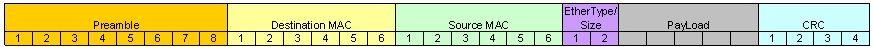
\includegraphics[width=16cm]{img/EthernetFrame.jpg}

\begin{description}
	\item[Präambel]: Zum Synchronisieren von Sender und Empfänger, \emph{Einschwingphase} (8 Byte)
	\item[SFD]: Festgelegte Sequenz 10101011 (1 Byte)
	\item[Ziel-Mac-Adresse]: Adresse des Empfängers (8 Byte)
	\item[Quell-Mac-Adresse]: Adresse des Senders (8 Byte)
	\item[VLAN-Tag]: Nach IEEE 802.1q, optional (4 Byte)
	\item[Typ-Feld]: Identifiziert die Art des nachfolgenden Inhalts, z.B. IP, ARP, etc...
	\item[Nutzlast]
	\item[PAD-Füllfeld]: Wird optional benötigt, um die Mindestlänge von 64 Byte einzuhalten \footnote{Rausfinden, warum mindestens 64 Byte nötig. Vermutung: Kollisionserkennung}
	\item[CRC-Prüfsumme]: Zur Fehlererkennung (4 Byte)
\end{description}

\subsubsection{CSMA/CD}

CSMA/CD regelt den Zugriff auf ein von mehreren Teilnehmern genutztes Medium (Kabel).
Dazu prüft der sendende Host, ob das Medium frei ist, bevor er sendet.
Beim Übertragen von Daten können Kollisionen erkannt werden.
Der Sendevorgang wird dann nach einer zufälligen Zeit wiederholt.
Aufgrund der verbreiteten Nutzung von Switches sind echte geteilte Medien inzwischen eher die Ausnahme.

$\Rightarrow$ Jeder Port am Switch bildet eine eigene \emph{Kollisionsdomäne}.
Die Bustopologie mit Koaxialkabeln (aber auch mit Hubs) wird nicht mehr genutzt.

\subsubsection{Duplex / Half Duplex}

Beim \textbf{Full Duplex} sind beide Seiten in der Lage, gleichzeitig zu Senden und zu Empfangen.
Im Falle von \textbf{Half Duplex} ist dies nur wechselseitig möglich (vgl Walkie Talkie).
Es sind verschiedene Realisierungen einer geteilten Nutzung eines Mediums möglich:

\begin{description}
	\item [Zeitduplex (TDD)]: Übertragung in verschiedenen Zeitschlitzen
	\item [Frequenzduplex (FDD)]: Übertragung auf verschiedenen Frequenzen
	\item [Codeduplex]: (nicht im Skript)
\end{description}

\subsection{Switching}

\textbf{Switches} sind Geräte auf dem OSI-Layer 2.
Sie empfangen Ethernet-Frames und leiten sie anhand ihrer Empfänger-MAC-Adresse weiter.
Im Gegensatz zum Hub wird dabei nur über den Port ausgegeben, hinter dem sich der Empfänger befindet.
Die Ausnahme ist hierbei, wenn der Port des Empfängers nicht bekannt ist.
Anhand der empfangenen Frames lernt ein Switch, wo sich Geräte befinden.

\subsubsection{Realisierungsmöglichkeiten}

%TODO Switches - Realisierungsmöglichkeiten

\subsubsection{Cut-Through und Store-and-Forward}

Beim \textbf{Cut-Through} (auch \emph{On The Fly Forwarding}) werden Pakete sofort nach Empfang der Empfängeradresse auf dem entsprechenden Port weitergeleitet, sofern dieser Frei ist.
Diese Methode ist sehr schnell (Verzögerung ca. 40$\mu$s), leitet jedoch gegebenenfalls auch fehlerhafte Frames weiter, da CRC umgangen wird.

\textbf{Store-and-Forward} hingegen empfängt zuerst den gesamten Frame, prüft diesen und leitet ihn anschließend weiter.
Offensichtlich werden keine fehlerhaften Pakete mehr in benachbarte Segmente weitergeleitet, dies wird jedoch durch erhöhte Latenz erkauft.

In der Praxis arbeiten Switches häufig im Cut-Through-Modus und schalten bei erhöhter Fehlerrate in den Store-and-Forward-Modus.

\subsubsection{VLAN}

Ermöglicht die Aufteilung von Switches in mehrere virtuelle LANs.
Den Ports werden dabei einzelne VLANs zugeordnet.
Auf diese Weise kann Hardware eingespart werden.
Realisiert wird dies mit einem 4 Byte langen Feld im Ethernet-Frame:
\begin{itemize}
	\item 2 Bytes \textbf{TPID} - Tag Protocol Identifier – Fester Wert 0x8100. Frame
	trägt die 802.1q/802.1p-Tag-Information
	\item 3 Bit \textbf{Priorität} (user\_priority) – Benutzer-Prioritätsinformationen
	\item 1 Bit \textbf{CFI} - Canonical Format Indicator – Gilt für alle vorhandenen
MAC-Adressinformationen im MAC-Datenpaket des Frames. Wert 0
das Format ist kanonisch (am wenigsten signifikante Bit zuerst); Wert
1 Format nicht-kanonisch. Benutzung im Token Ring/Source-Routed-
FDDI-Media-Zugang, um die Bit-Order der Adressinformationen des
verkapselten Frames festzulegen
	\item 12 Bit \textbf{VID} - VLAN Identifier – Identifizierung des VLANs zu dem der
Frame gehört
\end{itemize}
Erleichtert die Arbeit eines Administrators, da es viele Probleme von physikalischen Verbindungen umgeht. (bspw. Viel Hardware, unflexibel, Anpassungen nur mit hohem Aufwand)\\


\glqq Faulheit ist die Mutter der Ingenieurswissenschaften\grqq\\
\subsubsection{Trunking / Link Aggregation}
Ermöglicht die Zusammenfassung mehrerer Ports zur Erhöhung des Datensatzes.

\subsection{Asynchronous Transfer Mode}

\subsection{ATM}
	\begin{itemize}
		\item ATM kann als Protokoll für Internettelefonie eingesetzt werden und bietet eine geringe Latenz (von unter 200ms).
		\item Im Gegensatz zu Ethernet bietet ATM Garantien(!) und besitzt einen geringen Header von 5Byte. Es wird eine Leitung für den Datenstrom geschaltet.
		
	\end{itemize}

\subsection{Internet Protocol}
\label{subsec:ip}
Beim Internet Protocol handelt es sich um ein Layer-3-Protkoll, weches auf die Layer-2-Protokolle Ethernet, ATM und FDDI aufsetzen kann.
Es verwendet globale, logische Adressen.
Aufgrund der Erschöpfung des IPv4-Adressraumes\footnote{Weitere Maßnahmen, dem entgegenzuwirken sind etwa: NAT, CIDR, DHCP, Private Adressräume} (32 Bit) wird nach und nach IPv6 eingeführt (128 Bit)

\subsubsection{IPv4}
Wurde im RFC 791\cite{rfc791} definiert.
Der Header eines IPv4 Paketes ist insgesamt 20 Byte lang.
Davon sind insbesondere die folgenden von Interesse:

\begin{description}
	\item [Version]: In diesem Fall \emph{4}, bei IPv6 offensichtlich \emph{6} (4 Bit)
	\item [Header Length]: Gesamtlänge des Headers kann 20 Byte überschreiben, wenn zusätzliche Optionen gesetzt werden. Angabe in 32-Bit langen Blöcken (4 Bit)
	\item [Total Length]: Gesamtgröße des Pakets. Nach RFC muss jeder Host in der Lage sein, mindestens Pakete mit einer Länge von 576 Bytes zu verarbeiten. (16 Bit)
	\item [Type of Service]: Type of Service nach RFC791(ursprünglich für Quality-of-	Service-Anwendungen gedacht)
	
	\begin{itemize}
		\item bits 0-2: precedence
		\item bit 3: 0 = Normal Delay, 1 = Low Delay
		\item bit 4: 0 = Normal Throughput, 1 = High Throughput
		\item bit 5: 0 = Normal Reliability, 1 = High Reliability
		\item bits 6-7: Reserved for future use
	\end{itemize}
	Heute anders verwendet zur Servicebeschreibung durch Dienstklassen (DiffServ, 8 Bit)
	\item [Identification]: Falls ein Paket fragmentiert wird, haben alle Fragmente die	selbe Identification.
	\item [Flags]: Reserved\cite{rfc3514}, Don't Fragment, More Fragments (3 Bit)
	\item [Fragment Offset]: Kann ein Paket nicht auf einmal übertragen werden (z.B. bei
	kleinerer Maximum Transfer Unit, MTU), wird es fragmentiert.
	FO gibt an, ab welcher Stelle (gemessen in Blöcken von 8 Byte)
	dieses Paket die Daten enthält (MF Flag ist gesetzt) (13 Bit)
	\item[TTL]: Anzahl der Hops, bis Paket verworfen wird (wird bei jedem Routingvorgang reduziert)
	\item[Protocol]: Enthält für die darüber liegenden Layer Informationen, \glqq sodass diese etwas damit anfangen können\grqq
	\item[Checksum] wird selbst als 0 betrachtet, und fließt so nicht in die Kalkulation mit ein
	\item [Options]: Beispielsweise für Source Routing (Route ist im Paket vorgegeben); Sehr selten verwendet, häufig blockiert oder ignoriert
\end{description}

\begin{center}
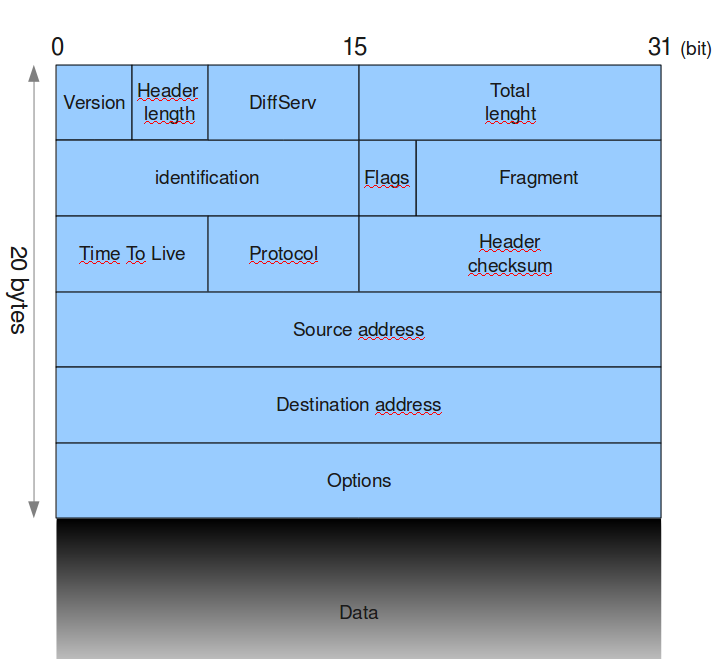
\includegraphics[width=8cm]{img/IP_packet}
\end{center}

Nutzung von Adressklassen\footnote{Class A 1.x.y.z-126.x.y.z; Class B 128.0.y.z-191.255.y.z; Class C 192.0.0.z-223.255.255.z} aufgrund der Verknappung der Adressen durch CIDR\cite{rfc1519} abgelöst.
Dies ermöglichte Super- und Subnetting.
Adressangabe bei CIDR im Format a.b.c.d/x, wobei x angibt, wie viele Bits zum Netz-Anteil der Adresse gehören.
Subnetze dienen zur Aufspaltung von Netzen in Teile, um diese besser handhaben zu können (Broadcast-Domains, Logische Strukturierung, Dezentrale Verwaltbarkeit)
\subsubsection{IPv6}

Die auffälligste Änderung von IPv4 zu IPv6 ist die vergrößerte Adressgröße (128 Bit).
Damit ergeben sich $3,4 \cdot 10^{38}$ Adressen.
IP - Adressen werden im Hexadezimalsystem zu je acht Word-Gruppen á 2 Bytes dargestellt.
Verkürzte Darstellung möglich durch Verzicht auf „Nullen“ in einer Gruppe (einmal je Adresse).
Es existieren IPv4-kompatible Adressen und die CIDR-Darstellung für Subnetze bleibt erhalten.
Weiterhin wurde die Anzahl der Felder im Header reduziert und (optionale) Erweiterungsheader hinzugefügt.
Wichtige Felder sind:

\begin{description}
	\item [Traffic Class]: \begin{itemize}
		\item 0 uncharakterisierter Verkehr
		\item 1 „Füllmaterial", z.B. Newsgroups
		\item 2 zeitunkritischer Verkehr, z.B. EMail
		\item 3 reserviert
		\item 4 Mengendaten, z.B. FTP, NFS
		\item 5 reserviert
		\item 6 Interaktive Anwendungen, z.B. telnet
		\item 7 Steuerung, z.B. SNMP
	\end{itemize}
	\item [Flow Label]: Anwendung kann Datenstrom mit einem Flow-Label versehen, z. B. bei Streaming-Anwendungen.
	Flow nicht notwendigerweise an Verbindung gebunden (logisch, da IP nicht verbindungsorientiert arbeitet).
	Empfänger kann Datenstrom am Flow Label erkennen. \cite{rfc3697, rfc6437}
	\item[Next Header]: Gibt an, dass ein weiterer Header folgt.
	In IPv6 sind viele Felder weggefallen.
	Next Header ermöglicht das Anfügen eines weiteren Headers.
	RFC 2460\cite{rfc2460} bietet beispielsweise:
	\begin{itemize}
		\item Hop – by – Hop Options Header
		\item Routing Header
		\item Fragmentation Header
		\item Authentication Header
		\item Encapsulated Security Payload (ESP) Header
		\item Destination – Option – Header
	\end{itemize}
	 
\end{description}

\begin{center}
	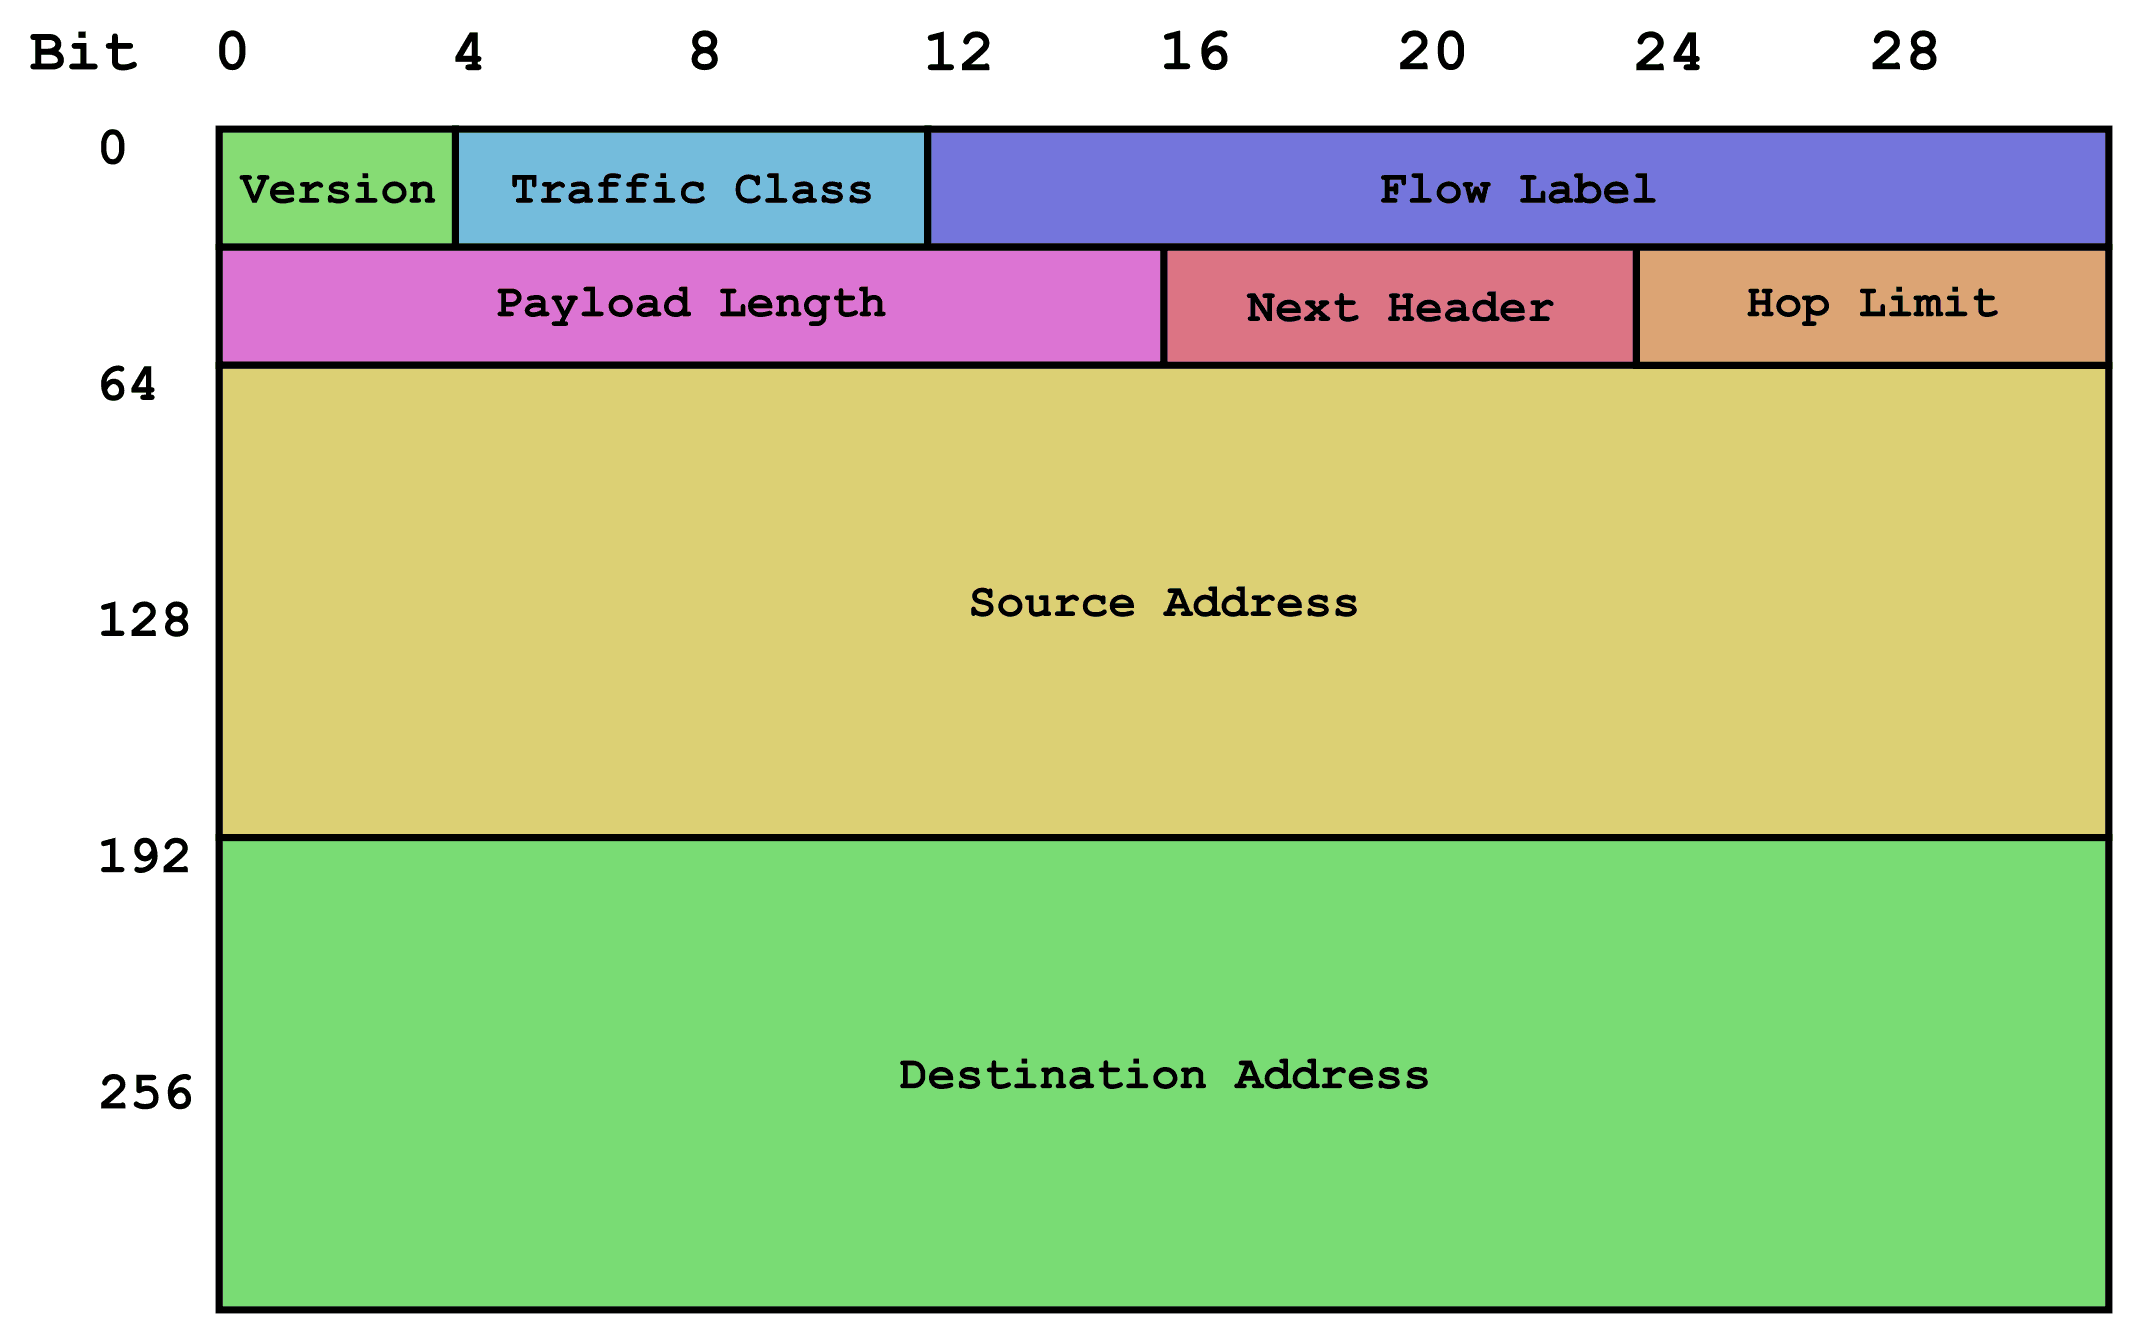
\includegraphics[width=10cm]{img/IPv6_header}
\end{center}

\subsubsection{Migration von IPv4 nach IPv6}

\emph{Wie migriert man Millionen von Hosts im Internet auf IPv6?}
Langsam, nach und nach.
Alle Hosts auf einmal sind nicht realisierbar.
RFC 1933\cite{rfc1933} schlägt drei Migrationsstrategien vor.

\begin{description}
	\item [Tunneling]: Zwischen zwei IPv6-Knoten wird ein virtueller Link aufgebaut.
	Die IPv6-Pakete werden (als Payload) in IPv4-Pakete verpackt und \emph{normal} über das Internet geroutet.
	\item [Dual Stack]: Auf Hosts und Routern werden sowohl IPv4 als acuh IPv6 eingerichtet.
	DNS kann A- oder AAAA-Records zurück geben, entsprechender Stack wird dann genutzt.
	%PRÜFEN Hier ist inhaltliche Überprüfung notwendig.
	Wird häufig mit Automatic Tunneling\footnote{\textquotedblleft IPv6-over-IPv4 tunneling where the IPv4 tunnel endpoint address is determined from the IPv4 address embedded in the IPv4-compatible destination address of the IPv6	packet.\textquotedblright} genutzt.
	
	Außerdem besteht die Möglichkeit von \textbf{Assignment of IPv4 Global Addresses to IPv6 Hosts} (AIIH).
	Dabei wird eine IPv4-kompatible IPv6-Adresse genutzt.
	Diese entspricht dem 96-bit Präfix 0:0:0:0:0:0, gefolgt von der IPv4-Adresse.
	Ist der Client der Dual-Stack-Hosts und der Server IPv4-only, verlangt der Client für die Dauer der Kommunikation eine	temporäre IPv4 Adresse beim AIIH Server (Kooperation von DNS und DHCPv6).
	Andernfalls (Client IPv4-only; Server Dual-Stack): DNS verlangt bei DHCPv6 eine temporäre IPv4 Adresse für Dual-Stack Host, welcher mit dieser rekonfiguriert wird.
	\item [Übersetzung der Header](Header Translation): Hierbei wird die IPv4 Unterstützung auf Systemen entfernt. Die IPv4-Pakete werden in IPv6-Pakete übersetzt; ein Translator übersetzt IP und ICMP Meldungen.
	%FRAGE Ist mit den Erweiterungsheadern das Options-Zeugs bei IPv4 gemeint?
	Erweiterungsheader werden nicht, oder nur bedingt übersetzt.
	Probleme entstehen, weil sich einige Felder nicht immer übersetzen lassen und Adressumwandlung Datenbanken-Lookups erfordern.
\end{description}


\subsection{User Datagram Protocol}

Bei UDP handelt es sich um ein Layer-4-Protokoll.\cite{rfc768}
Es dient zur Übermittlung kurzer Nachrichten an andere Systeme und garantiert weder Zuverlässigkeit noch Einhaltung der Reihenfolge der Pakete beim Empfänger.
Die Adressierung geschieht über Ports (16 Bit).
Der Header enthält 4 Felder (je 16 Bit): Quellport, Zielport, Datagram-Länge und eine Checksumme.

\subsection{Transmission Control Protocol}
 %TODO TCP Slow start wird bei HTTP erwähnt, hier nochmal kurz erklären?
TCP ist ebenfalls ein Layer-4-Protokoll.\cite{rfc793}
Es garantiert eine Ankunft der Pakete in korrekter Reihenfolge.
Clienten sehen die Verbindung als bidirektionalen Datenstrom, tatsächlich findet die Kommunikation über Pakete statt. Die Kommunikation erfolgt durch TCP zustandsbehaftet.
TCP arbeitet byte-orientiert.

\subsubsection{Paketstruktur}

Der Header des TCP-Fragments ist 20 Byte groß.
Wichtige Felder sind:
\begin{description}
	\item [Sequence Number / Acknowledgement Number]: Zerlegung des Datenstroms in nummerierte Blöcke.
	Größe der Blöcke ist variabel (Nagle Algorithmus).
	Verwerfen von Segmenten mit fehlerhafter Prüfsumme.
	Bestätigung empfangener Segmente.
	Nicht unbedingt für jedes Segment einzeln (Windowing).
	Erneuter Transport unbestätigter Segmente.
	Zusammensetzung des Datenstroms auf Empfängerseite
	
	\item [Flags]: dienen unter anderem zur Steuerung des Verbindungsauf- und –abbaus.
	\begin{description}
		\item [URG] - Urgent Flag (Urgent Pointer enthält
			Sequenznummer, die bevorzugt übertragen werden soll)
		\item [ACK] – Acknowledgement
		\item [PSH] – Push (Paket wird sofort an Anwendung weitergeleitet, ohne Zwischenpuffer)
		\item [RST] – Reset (Unterbrechung der Verbindung)
		\item [SYN] – Synchronized (Aufbau der Verbindung)
		\item [FIN] – Finish (Beenden der Verbindung)
	\end{description}
	\item [Window Size]: Anzahl der Daten, die gesendet werden können bis ein Acknowledgement gesendet werden muss (in Bytes oder mit speziellem Option Header nach RFC1323 \cite{rfc1323} auch bis zu 1GB,	dann Linksverschiebung um bis zu 14 Bits, $2^{14} \cdot 64k = 1G$).
\end{description}

\subsubsection{Zustände}

Zum Aufbau einer Verbindung wird der \textbf{3-Way-Handshake} durchgeführt:
\begin{enumerate}
	\item $\rightarrow$ SYN
	\item $\leftarrow$ SYN + ACK
	\item $\rightarrow$ ACK
\end{enumerate}
Ein Timeout findet typischerweise nach 75 Sekunden statt. Zum Abbau der Verbindung genügt das Senden und Quittieren eines FIN.

\subsubsection{Sliding Window \& Nagle-Algorithmus}
%PRÜFEN Sliding Window & Nagle Algorithmus

\textbf{Hinweis:} Konnte in den Folien hierzu nix groß finden, Infos stammen aus dem Tanenbaum\footnote{Das Kapitel heißt in der deutschen Fassung ernsthaft \emph{TCP-Schiebefenster}. Barbaren!}\cite{tanenbaum2003computer}.

Die Flusskontrolle von TCP funktioniert im Groben folgendermaßen:
Nach Erhalt der Daten quittiert der Empfänger das letzte Empfangene Segment im \texttt{ACK}-Feld.
Empfängt er beispielsweise eine 2kB große Nachricht mit den Segmenten 0 - 2048, sendet er \texttt{ACK=2048}.
Gleichzeitig ermöglicht das \textbf{Window Size} (WIN) Feld eine Angabe, wie viele Segmente der Empfänger noch annehmen kann, etwa weil er nur einen begrenzt großen Puffer hat, der erst gelesen und geleert werden muss.

Bei \texttt{WIN=0} wird dem Sender signalisiert, dass der Puffer des Empfängers voll ist und keine Daten empfangen werden können.
Ausnahmen sind hier priorisierte Nachrichten und \emph{window probes}\footnote{Fenstersondieranfragen}.
Letztere fordern den Empfänger dazu auf, wiederholt das nächste erwartete Byte und die Fenstergröße zu übermitteln, um Deadlocks vorzubeugen.

Es muss nicht zwingend jedes TCP-Segment einzeln bestätigt werden.
Anwendungen, wie Telnet oder SSH etwa, könnten für jeden Tastaturanschlag ein einzelnes Segment verschicken, was eigentlich zu bestätigen ist.
Stattdessen werden hier häufig \text{verzögerte Bestätigungen} eingesetzt.
Dabei kann bis zu 500ms auf weitere eintreffende Daten gewartet werden, die dann gleich mitbestätigt werden.

Da der durch viele kurze Pakete erzeugte Overhead die Effizienz der Kommunikation negativ beeinflusst, wird häufig der \textbf{Nagle-Algorithmus} eingesetzt.
Hierbei wird, wenn die Daten vom Sender byteweise kommen, immer nur das erste Byte gesendet und die nachfolgenden Nachrichten im Puffer gehalten.
Wird das erste Byte bestätigt, so werden alle sich im Puffer befindlichen Daten gesendet.
So werden viele kleine Daten in großen Segmenten zusammengefasst.
Aufgrund der Verzögerung kann diese Technik auch unerwünschte Folgen haben, etwa bei Spielen oder Konsolenanwendungen.


\subsection{SCTP}
%PRÜFEN SCTP
Das \textbf{Stream Control Transmission Protocol}\cite{rfc4960} ist ein zuverlässiges (Reihenfolge, Duplikate, Veränderungen, Fehlende Daten) Transportprotokoll für Unicast-Kommunikation.
Es arbeitet nachrichten-orientiert, die Nachrichten\footnote{Auch als Chunks bezeichnet} haben eine interne Struktur.
SCTP ermöglicht multi-streaming, Daten können in parallelen Streams übertragen werden.
Dies ist beispielsweise dann hilfreich, wenn Websiten mit mehreren Ressourcen übertragen werden.
Streams werden einzeln nummeriert (Retransmits müssen nur für den jeweiligen Stream erfolgen).
Daten-Chunks können einzeln bestätigt werden. (\textbf{Selective ACK})
Retransmits nur für fehlende Pakete.

Es bietet \textbf{Schutz gegen SYN Flooding} (Cookie-Mechanismus) - Anfrager bekommt Cookie und muss das nachfolgend wieder vorweisen, dies bedeutet keinen Ressourcenverbrauch beim Server:
Der Server speichert dazu bei einer Verbindungsanfrage (\texttt{INITPaket}) keine Zustandsinformationen, sondern schickt diese in Form eines Cookies (\texttt{INIT-ACK-Paket}) an den Client.
Der Client muss dieses Cookie in seine Antwort (\texttt{COOKIEECHO}-Paket) einfügen und wird damit vom Server als zum Verbindungsaufbau berechtigt erkannt.
Eine Bestätigung geschieht durch ein \texttt{COOKIE-ACK}-Paket.

SCTP ermöglich \textbf{Multi homing}.
Dabei haben beide Kommunikationspartner eine primäre und potentiell mehrere sekundäre (IP-)Adressen.
Auf diese Weise ist es möglich, eine stabile Verbindung aufrecht zu erhalten, auch wenn ein Interface inaktiv wird.
Offensichtlich können hierbei die Nachrichten unterschiedliche Pfade nutzen.
\subsubsection{Paketaufbau}
Ein allgemeines Paket besteht aus einem \textbf{Common Header} und mehreren nummerierten \textbf{Chunks}.
Der Header besteht aus \textbf{Source-} und \textbf{Destinationport}, einem \textbf{Verification Tag} und einer \textbf{Checksum}.
Chunks bestehen aus einem \textbf{Typen}, einer Reihe von \textbf{Flags}, einem \textbf{Längenfeld}, sowie dem \textbf{Wert (Value)}.
Letzteres setzt sich, je nach Chunk-Type, aus mehreren Feldern zusammen.
Weiter unten wird zur Veranschaulichung ein Payload Data Chunk beschrieben.

Der Typ des Chunks wird durch das 8-Bit lange Type-Feld bestimmt.
Dafür sind die Werte 0-254 verfügbar.
Wert 255 ist für eine zukünftige Erweiterung des Feldes reserviert.
Im Folgenden einige Beispiele für Typenfelder.
Weitere Werte sind verfügbar oder bereits reserviert.
\begin{multicols}{2}
	\begin{enumerate}
		\setcounter{enumi}{-1}
		\item Payload Data \texttt{DATA}
		\item Initiation \texttt{INIT}
		\item Initiation Acknowledgement \texttt{INIT ACK}
		\item Selective Acknowledgement \texttt{SACK}[sic!]
		\item Heartbeat Request \texttt{HEARTBEAT}
		\item Heartbeat Acknowledgement \texttt{HEARTBEAT ACK}
		\item Abort \texttt{ABORT}
		\item Shutdown \texttt{SHUTDOWN}
		\item Shutdown Acknowledgement \texttt{SHUTDOWNACK}
		\item Operation Error \texttt{ERROR}
		\item State Cookie \texttt{COOKIE ECHO}
		\setcounter{enumi}{13}
		\item Shutdown Complete \texttt{SHUTDOWN COMPLETE}
	\end{enumerate}
\end{multicols}


Das \textbf{Verification Tag} im Header wird vom Empfänger genutzt, um den Sender des Pakets zu validieren.
Es entspricht dem Wert des Initiate Tag\footnote{Das Initiate Tag ist ein Feld im \texttt{INIT Chunk}.}.
\textbf{Ausnahmen:} Beinhaltet das Paket einen \texttt{INIT Chunk}, ist das Verification Tag Null.
Wenn ein Paket einen \texttt{SHUTDOWN COMPLETE Chunk} enthält, bei dem das T-Bit gesetzt ist, so wird das Verification Tag vom \texttt{SHITDOWN ACK chunk} kopiert.
Zu guter Letzt wird das Verification Tag eines \texttt{ABORT chunks} vom ABORT-verursachenden Paket übernommen.

\textbf{Payload Data} Chunks sollen im Folgenden kurz besprochen werden.
Sie haben den Type-Wert 0.
Im Flag-Feld sind die letzten 3 Bits von besonderem Interesse, gefolgt vom Längen-Feld.
Die Flags haben haben die folgende Bedeutung:
\begin{description}
	\item[U] | Ist das \emph{Unordered} Bit gesetzt, wird die Stream Sequence Number ignoriert.
	Das bedeutet, dass empfangene Chunks, ohne vorher sortiert zu werden, an den darüberliegenden Layer weitergereicht werden.
	Ist eine Nachricht fragmentiert, so wird dieses Bit bei jedem Fragment gesetzt.
	\item[B] | Das \emph{Beginning} fragment Bit gibt an, dass es sich um das erste Fragment einer Nachricht handelt
	\item[E] | Das \emph{Ending} fragment Bit gibt an, dass es sich um das letzte Fragment einer Nachricht handelt.
\end{description}
Das Value-Feld ist beim DATA Chunk wie folgt aufgebaut:
\begin{description}
	\item[Transmission Sequence Number (TSN)] | enthält einen Wert zwischen 0 und $2^{32}-1$.
	Sie identifiziert einen Chunk und wird zur Bestätigung des Erhalts genutzt.
	Nach erreichen des maximalen Wert beginnt die Nummerierung wieder bei 0.
	\item {Stream Identifier S} | identifiziert den Stream, zu dem der Chunk gehört.
	Dies ist notwendig, wenn parallele Streams versendet werden.
	\item {Payload Protocol Identifier} | identifiziert das genutzte Protokoll.
	Das Feld wird von SCTP selbst nicht genutzt, sondern nur an höhere Schichten weitergereicht, beziehungsweise von Zwischenstationen interpretiert.
	\item {User Data} | enthält letztendlich die zu transportierenden Daten.
\end{description}


\section{Adressierung}
% 030
\subsection{MAC-Adressen}

\begin{itemize}
	\item Layer-2-Adressen für Ethernet
	\item 6 Byte / 48 Bit groß
	\item \emph{Eigentlich} weltweit eindeutig
	\item \emph{Eigentlich} in Hardware gegossen, trotzdem fälschbar
	\item Darstellung: Hexadezimal, Bits getrennt durch [.:-]
	\item Bit 3 bis Bit 24 an Hersteller gebunden (z.B. 00-60-2F-xx-xx-xx für Cisco)
	\item Broadcast: FF-FF-FF-FF-FF-FF 
\end{itemize}

\subsection{VPI und VCI bei ATM}
ATM beruht auf Verbindungen, die sowohl fest eingerichtet oder nur für eine bestimmte Zeit geschaltet werden können. Für diesen Zweck wurden Virtual Paths (VPs) und Virtual Channels (VCs) definiert. Jede ATM-Zelle enthält im Header einen Virtual Path Identifier (VPI, 8 bzw. 12 Bit) und einen Virtual Channel Identifer (VCI, 16 Bit).\\
Ein ATM-Paket besteht aus 5 Byte Headerund 48 Byte Nutzlast. Es gibt zwei Arten von ATM-Paket-Formaten:
	\begin{enumerate}
		\item NNI (Network-Network-Interface)\\
		Wird von öffentlichen ATM-Netzen verwendet.	
		\item UNI (User-Network-Interface)\\
		Wird für private ATM-Verbindungen genutzt. UNI besitzt ein GFC-Feld für eine (bis heute undefinierte) lokale Flusskontrolle zwischen Netz und User.
	\end{enumerate}
\subsection{IP-Adressen}

Siehe Abschnitt \ref{subsec:ip}.

\subsection{Ports}

Für die Layer-4-Protokolle UDP und TCP werden 16-Bit-Adressen verwendet.
Diese werden als Ports bezeichnet.
Ports 0-1023 sind dabei standardisiert.
Wichtige Portnummern sind beispielsweise:
\begin{center}
\begin{tabular}{|c|c|c|c|}
	\hline Port & TCP & UDP & Beschreibung \\ 
	\hline 20 & Ja & Nein & FTP - Datenübertragung \\ 
	\hline 21 & Ja & Nein & FTP - Kontrolle \\ 
	\hline 22 & Ja & (Ja) & SSH \\ 
	\hline 23 & Ja & Nein & Telnet \\ 
	\hline 25 & Ja & Nein & SMTP \\ 
	\hline 53 & Ja & Ja & DNS \\ 
	\hline 80 & Ja & Nein & HTTP \\ 
	\hline 110 & Ja & Nein & POP3 \\ 
	\hline 123 & Nein & Ja & NTP \\ 
	\hline 443 & Ja & Nein & HTTPS \\ 
	\hline 
\end{tabular} 
\end{center}
\subsection{URIs, URNs und URLs}
\begin{description}
\item [Uniform Resource Identifier]: String; Benennt oder identifiziert eine Ressource z.B.  \textbackslash\textbackslash139.30.3.23\textbackslash iukp\textbackslash beispiel.txt
\item [Uniform Resource Name]: Sonderform der URI, die eine Ressource in einem bestimmten
Namespace benennt | urn:ip-addr:139.30.3.23
\item [Uniform Resource Locator]: Sonderform der URI, die zusätzlich das Protokoll angibt, über das die Ressource erreichbar ist z.B. http://139.30.3.23/beispiel.txt
\end{description}
\subsection{*cast} 
\begin{description}
	\item[Unicast]: Einer sendet an einen, wie beispielsweise in einer TCP-Verbindung für HTTP. Adressierung durch Angabe des Empfängers.
	\item[Broadcast]: Einer sendet an alle, wie beispielsweise in ARP oder DHCP. Hierzu werden spezielle Adressen (MAC: FF-FF-FF-FF-FF-FF; IP: höchste Adresse im Subnetz) verwendet. Broadcastbereiche sollten möglichst klein gehalten werden, um möglichst wenig Teilnehmer zu belästigen.
	\item[Multicast]: Einer sendet an viele Mitglieder einer Gruppe. Siehe Abschnitt \ref{sec:muliticast}.
	\item[Concast]: Viele senden an einen, Nachrichten werden so früh wie möglich zusammengefasst. Verhindert Implosion, Überlastung des Empfängers. Beispielswiese sinnvoll, wenn Fehlermeldungen zusammengefasst werden können. Keine direkte Unterstützung in IP, MAC, Ethernet
\end{description}

\subsection{ICMPv6 Neighbor Discovery Protocol (NDP)} 
\begin{itemize}
	\item Dient als Ablösung von ARP
	\item Mechanismus von IPv6 für Auflösung (Übersetzung) von Netzwerkadressen in Hardwareadressen\cite{rfc4861}.
	\item Es existieren verschiedene Typen:
		\begin{itemize}
		\item Router Solicitation – Type 133 \\
		Alle Router im selben Netz werden aufgefordert, sich zu melden und senden an Router-Multicast-Adresse 
		\item Router Advertisement – Type 134 \\
		Router verkünden Anwesenheit im Netz, periodisch oder als Antwort auf \textit{Router Solicitation} 		
		\item Neighbor Solicitation – Type 135 \\
		Zur Auflösung von IPv6-Adressen zu Link-Layer-Adressen. Umgesetzt als Broadcast an Link-Layer-Broadcast-Adressen.
		\item Neighbor Advertisement – Type 136 
		\item Redirect – Type 137 \\
		Router teilt mit, dass es besseren next hop gibt 
		\end{itemize}
	
	
\end{itemize}
%290


\subsection{Domainverwaltung}
\begin{itemize}
	\item Adressierung mit Hilfe von IP-Adressen ist für menschliche Nutzer sehr unpraktisch. Daher werden Namen zur Adressierung verwendet.
	\item Namen sind in einem paketvermittelten Netzwerk unpraktikabel. Daher ist eine Umwandlung der Namen in IP-Adressen notwendig.
	\item Domain Name Service (DNS) erledigt diese Aufgabe.
	\item Verteilung der Verantwortlichkeiten.
	\begin{itemize}
		\item Keine einzelne Institution verwaltet alle Namen im Baum.
		\item NIC verwaltet die Top-Level Domain.
		\item Die Verwaltung der unteren Ebenen wird entsprechend verteilt.
	\end{itemize}
	\item Wird die Verantwortung für eine Zone delegiert, dann ist die entsprechende „Person“ für diese Zone verantwortlich (Zerlegung der Aufgabe in kleinere Teilaufgaben).
	\begin{itemize}
		\item Zuordnung von Namen und IP-Adressen.
		\item Betrieb von Primary Name Server und mindestens ein Secondary Name Server.
	\end{itemize}
\end{itemize}
\subsection{Informationen in der Domain Registry}
\begin{itemize}
	\item IPv4-Adressen (A-Records)
	\item IPv6-Adressen (AAAA-Records)
	\item Adresse des Mail-Servers (MX-Records)
	\item Referenzen auf andere Einträge (CNAME)
\end{itemize}

\section{ARP, RARP}

% Ende 030, 040

ARP wandelt Layer-3-Adressen in Layer-2-Adressen um.
Es beschränkt sich nicht auf das Erfragen von MAC-Adressen zu IP-Adressen, sondern ermöglicht beispielsweise auch ATM ARP, IP over FDDI und IP over Token Ring.
\begin{itemize}
	\item Erfragt für gegebene IP-Adresse eine MAC-Adresse.
	\item Host erzeugt Broadcast.
	\item Der angefragte Host darf darauf antworten (Unicast).
	\item Nachdem der Sender der Broadcast-Nachricht die Antwort erhalten hat, kann er die IP-Adresse der Ethernet-Adresse zuordnen.
	\item Diese Ethernet-Adresse wird dann für alle folgenden Pakete an diese Internet-Adresse verwendet, solange bis die Cache-Zeit abgelaufen ist.
	\item RFC 826 \cite{rfc826}
\end{itemize}

\subsection{Einsatzfälle}

\begin{enumerate}
	\item Zwei Hosts möchten im selben Netzwerk (ausschließlich Layer 2) miteinander kommunizieren und kennen nur die Layer-3-Adresse (z.B. IP-Adresse) des Empfängers.
	\item Ein Host benötigt die Layer-2-Adresse des Gateways, um andere Netze zu erreichen (Sonderfall des zuvor genannten)
	\item Zwei Gateways wollen kommunizieren.
\end{enumerate}

\subsection{Paketstruktur}
Wichtige Felder eines ARP-Requests sind:
\begin{description}
	\item[Hardware type]: Kennzeichen für die verwendeten Hardware-Adressen (1 für Ethernet, 2 Byte)
	\item[Protocol type]: Kennzeichen für die verwendeten Protokoll-Adressen (L3) (0x0800 für IPv4, 2 Byte).
	\item[Hardware length]: Länge der Hardware-Adresse in Bytes (6 für Ethernet, 1 Byte)
	\item[Protocol Length]: Länge der Protokoll-Adressen (L3) (4 für IPv4, 1 Byte)
	\item[Operation]: Unterscheidung von 1 Request und 2 Reply, da für beides gleiche Pakete verwendet werden (2 Byte, warum zur Hölle reserviert man für 2 Werte 2 Byte?)
\end{description}

Es folgen Sender hardware address, Sender protocol address, Target hardware address und Target protocol address

\subsection{ARP-Caching}

Um nicht für jedes IP-Paket einen neuen ARP Request zu stellen, werden die Ergebnisse zwischengespeichert.
Typischerweise 10 Minuten lang.
Kommt es während der Cache-Zeit zu einem Fehler (Host nicht erreichbar), wird erneut ein ARP-Request ausgeführt.

\subsection{ARP-Announcements}

Der anfragende Host sendet bekanntlich einen Broadcast, alle Host im gleichen Netz können folglich diese Information ebenfalls verwenden, und auf diese Weise eigene Anfragen sparen.
Anwendungen:
\begin{itemize}
\item Unterbrechungslose Übernahme einer Protokoll-Adresse (z.B. IP-Adresse) in hochverfügbaren Systemen.
\item Der anfragende Host kann auf diese Weise feststellen, ob eine Protokoll-Adresse bereits vergeben ist (Gratuitous ARP). Dieser Mechanismus wird bei IP-Autoconf verwendet.
\end{itemize}

IP-Autoconf \cite{rfc3927} ist eine einfache Möglichkeit zur Adresskonfiguration ohne Server (DHCP, RARP).

\begin{itemize}
	\item Host wählt zufällig eine Adresse.
	\item Überprüft mittels Gratuitous ARP, ob diese Adresse bereits vergeben ist.
	\item Falls ja, andere Adresse zufällig wählen und erneut überprüfen.
	\item Falls nein, Adresse benutzen und andere ARP Requests für diese Adresse beantworten.
\end{itemize}

\subsection{ARP-Spoofing}

Da ARP nicht kryptografisch abgesichert ist, kann jeder Host auf ARP Requests antworten oder ARP Announcements erzeugen.
Ziel ist das Umleiten von Datenpaketen.
Es gibt Programme, die Änderungen der Hardware-Adressen erkennen (z.B. arpwatch).
Der Administrator muss dann die Ursache überprüfen

\subsection{Proxy ARP}

Wird von speziellen Routing-Protokollen verwendet.
Jeder Nachbar (One-Hop-Neighbor), der auf der Route zum Ziel liegt, beantwortet einen eintreffenden ARP-Request mit seiner Hardware-Adresse.
Pakete werden so von Host zu Host weitergeleitet

\subsection{Reverse RP}

Erfragt eine IP-Adresse bei bekannter MAC-Adresse und ist nicht unbedingt für die Funktionsfähigkeit von IP über Ethernet notwendig.
RARP wird in RFC 903 \cite{rfc903} standardisiert.
Haupteinsatzzweck ist die automatische Konfiguration der Protokoll-Adresse.
Dabei sendet der Host einen RARP-Request mit der eigenen Hardware-Adresse (z.B. MAC).
Ein RARP-Server beantwortet diesen Request und liefert die hinterlegte Protokoll-Adresse (z.B.IP).
Da RARP Link-Local-Broadcasts verwendet, ist ein RARP-Server pro Netz notwendig.
Benutzt gleiche Paketstruktur wie ARP, lediglich anderen EtherType\footnote{Feld im Ethernet-Header, siehe Abschnitt \ref{subsec:ethernet}} (0x8035)

\section{DNS und WHOIS}

% 050
%TODO Ordnung in die Informationen bringen. Folien haben keinen guten roten Faden
Die Aufgabe des Domain Name Systems ist die Übersetzung von (Layer-4) IP-Adressen in, für den menschlichen Gebrauch besser verwendbare Namen.
Der Name wird dabei aus hierarchischen Domains, getrennt durch Punkte (.) zusammengesetzt.\\
Direkt unter der Wurzel steht hierbei die sogenannte Top-Level-Domain.
Bei Top-Level-Domains wird zwischen \textbf{länderspezifischen} (ccTLD) und \textbf{generischen} (gTLD) Domains unterschieden.
Während erstere, bestehend aus zwei Buchstaben, durch lokal verantwortliche Institutionen\footnote{Network Information Centers z.B. DENIC für .de} verwaltet werden, werden gTLD durch die \textbf{ICANN} oder beauftragte Institutionen vergeben.
%TODO 050_DNS.pdf hat hier noch so eine komische Seite 61
Bei der Vergabe gilt das \emph{first come, first serve}-Prinzip.
Für die Namensbildung gelten gewisse Regelungen, z.B. Ziffern 0-9, Bindestriche, Buchstaben, sowie einige ausgewählte lokale Buchstaben.
Letztere müssen ASCII-kodierbar sein (ACE)\cite{rfc3490}.
Jede (Teil-) Domain ist maximal 63 Zeichen lang, insgesamt ist der vollständige Pfad jedoch 255 Zeichen lang.
Folgende Daten sind bei der Domainanmeldung von Interesse:

\begin{description}
	\item[Domaininhaber](Holder): Person, der die Domain \emph{gehört}
	\item[Administrativer Ansprechpartner]: Vom Inhaber Bevollmächtiger, darf alle Entscheidungen treffen (Admin-C)
	\item[Technischer Ansprechpartner, Zonenverwalter]: Typischerweise Kontaktadresse der Firma, die die Domain betreibt (Tech-C, Zone-C)
	\item [Technische Daten]: z.B. Nameserver
\end{description}

Hoster tragen oft nicht den Inhaber selbst als Admin-C, sondern sich selbst ein.
Außerdem stellen sie in der Regel den Nameserver zur Verfügung.
Die Registrierung einer Domain gilt immer für einen bestimmten Zeitraum.
Ein Wechsel erfordert eine Freigabe beim alten Provider durch Inhaber oder Admin-C.

\subsection{Weiteres Bla zu DNS}

Beim Domain Name System handelt es sich um ein \textbf{sehr großes}, \textbf{hierarchisch strukturiertes}, \textbf{verteiltes}, \textbf{repliziertes} und \textbf{lokal verwaltetes System} \cite{rfc1034,rfc1035}.
Aus dem hierarchischen Benennungsschema resultiert das verteilte Datenbanksystem des DNS.
Jede Domain bestimmt selbst, wie die unter ihr liegenden Domains zugewiesen werden, hat dementsprechend eigene Verantwortlichkeiten.
Ist ein Namensserver für eine solche Zone verantwortlich, kann er Anfragen autoritativ beantworten(Autoritäskonzept).
Andernfalls wird die Anfrage aus dem Cache beantwortet oder an einen anderen Nameserver delegiert (Delegationskonzept).
Das kann der Nameserver einer Subdomain oder (default) ein Root Name server sein.\\
Die Aufteilung in die Zonen erfolgt anhand von Punkten - Bsp: www.spiegel.de

\subsection{Servertypen}

\begin{description}
\item[Primary Server]: Ist Hauptserver einer Domain und autorisiert, Anfragen zu seiner Domain verbindlich zu
beantworten.
Er verfügt über alle Daten dieser Domain, welche in Zonen-Dateien abgelegt sind, die der Verwalter des
Servers erstellt
\item[Secondary Server]: Ist ebenfalls autorisiert, verbindliche Antworten zu seiner
Domain zu liefern, lädt die Domain-Datenbank von einem Primary Server und aktualisiert sie bei Bedarf
\item[Caching-only Server]: Verfügt über keine eigenen Domain-Informationen.
Fragt bei dem für die Domain zuständigen Primary oder Secondary Server nach und speichert die Antwort zwischen.
Ist zur Beantwortung von Anfragen zu einer Domain „nicht autorisiert“ (kann die Genauigkeit und Aktualität nicht gewährleisten)
\item[Slave	Server]: Reicht alle Anfragen, die er selbst nicht aus seinem eigenen Cache beantworten kann, an eine zuvor festgelegte Liste von anderen Servern (Forwarders) weiter.
Forwarders fragen ihrerseits den zuständigen Server und speichern Ergebnis zwischen (Caching)
\end{description}

%TODO DNS ist noch nicht fertig


\section{Timeouts, ACK, Bestätigungen}
	\subsection{Begriffe}
	\begin{itemize}
		\item \textbf{Positive Bestätigung}
		\begin{itemize}
			\item Bestätigung, wenn ein Protokollschritt erfolgreich ausgeführt wurde.
			\item Wartezeit ist ein Nachteil.
			\item Reaktion auf verloren gegangene Bestätigungen muss
			vorgesehen werden.
		\end{itemize}
		\item \textbf{Negative Bestätigung}
		\begin{itemize}
			\item Fehlermeldung, wenn ein Protokollschritt nicht erfolgreich war.
			\item Ausbleiben der Fehlermeldung ist nur eine notwendige
			Bedingung, keine hinreichende, dafür, dass Protokollschritt
			erfolgreich war.
		\end{itemize}		
		\item \textbf{Timeouts}
		\begin{itemize}
			\item Ein Kontrollsignal in einem technischen System, das die Überschreitung der normalerweise für eine Aktion benötigten Zeit anzeigt. Damit sollen unkontrollierte Zustände (Warten, Endlosschleifen) verhindert und die Systemressourcen geschont werden.\cite{timeout}
		\end{itemize}		
		\item \textbf{Acknowledgements}
		\begin{itemize}
			\item Ein ACK dient der Bestätigung eines empfangenen Datenpakets.
		\end{itemize}
	\end{itemize}
	
	\subsection{TFTP - Trivial File Transfer Protocol}
	\begin{itemize}
		\item TFTP ist ein vereinfachtes Datei-Übertragungs-Protokoll, das auf UDP aufbaut (FTP verwendet TCP) \cite{rfc1350}.
		\item Das Ziel von TFTP ist zum einen ein einfacher \textbf{Datentransfer} und zum anderen das Ermöglichen des \textbf{Bootens einer Workstation} ohne Diskettenlaufwerk.
		\item An TFTP gestellte Anforderungen sind, dass es kompakt sein soll (um ins ROM zu passen), keine Authentifikation.
		\item TFTP ist ein stop-and-wait Protokoll.
		\begin{itemize}
			\item Kein neuer Protokollschritt, solange nicht der vorhergehende erfolgreich (korrekt) abgeschlossen ist.
			\item Niedrige Protokoll-Leistung (Datendurchsatz).
			\item Dafür einfache Implementierung.
			\item Geänderte Reihenfolge stellen kein Problem dar, da stopand-wait Protokoll nur jeweils ein Paket hängig hat.
		\end{itemize}
		\item Alternative
		\begin{itemize}
			\item Positive Bestätigung kann verzögert werden (sliding window).
			\item Übersendung mehrerer Pakete und dann erst warten auf eine Bestätigung.
			\item Höherer Datentransfer (Beispiel TCP).
		\end{itemize}
		\item Doppelte Pakete werden aufgrund der Blocknummer erkannt, während verlorene Pakete über Timeout beider Partner erkannt werden.
		\item TFTP Nachricht hat keine Checksumme, Datenveränderungen müssen durch die UDP-Checksumme abgefangen werden.
		\item Retransmission Timer
		\begin{itemize}
			\item Wert sollte je timeout um bestimmten Faktor multipliziert werden (sog. Exponential backoff).
			\item Retransmission timeout je Paket = 5 s.
			\item Retransmission timeout für \glqq Verbindung\grqq = 25 s.
		\end{itemize}
	\end{itemize}
	\begin{center}
		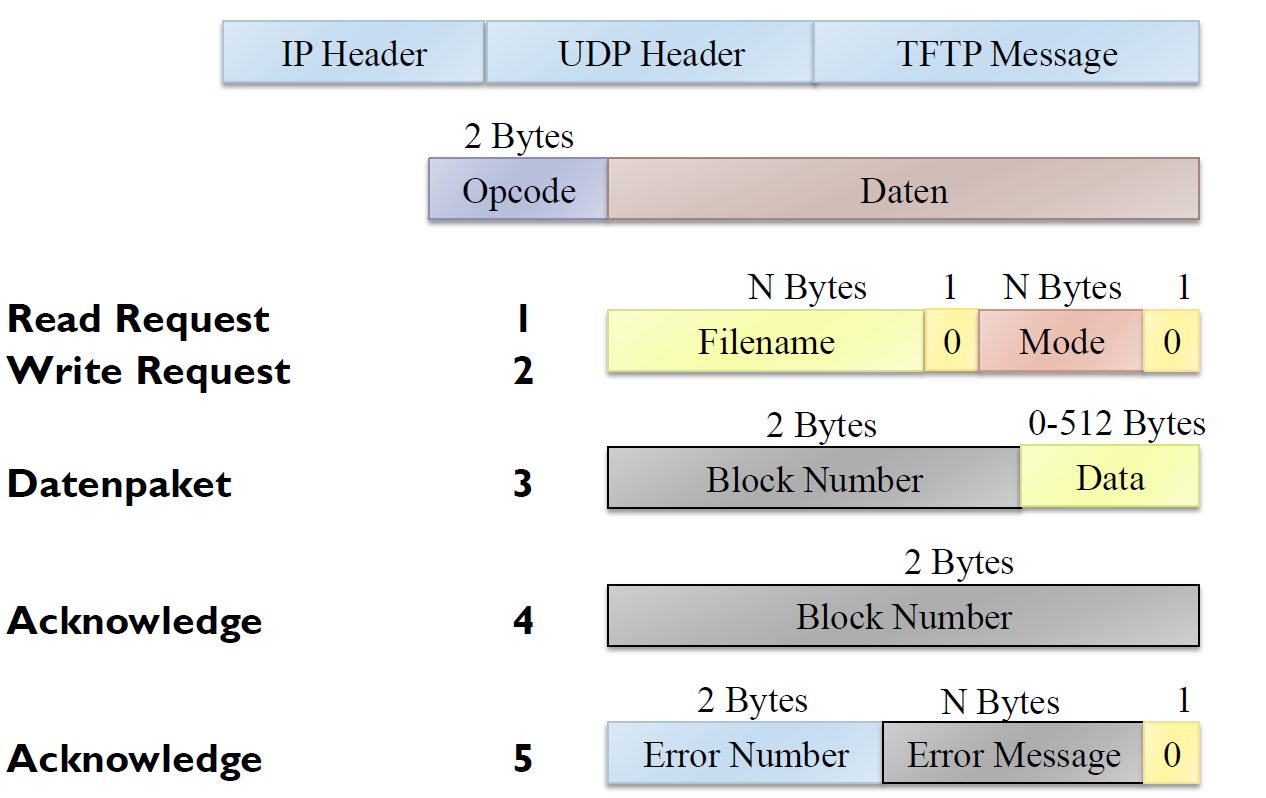
\includegraphics[width=10cm]{img/tftp.png}
	\end{center}
	
	
% 070

\section{Routing}

% 080, 090, 095, 100, 110, 120, 130
Routing optimiert den Weg zum Ziel einzelner Pakete.
Dabei gewährt es Dienstgüten (z.B. Konstante Latenz, Bitrate, Durchsatz, sowie Priorisierung von Paketen) und minimiert Kosten.

\subsection{Begriffe}
\begin{description}
	\item[Router] - Gerät, welches mindestens zwei unterschiedliche Netzwerke verbindet.
					Ist in der Lage, den besten Weg für eine Nachricht durch ein Netzwerksystem bis zum Empfänger zu bestimmen.
	\item[Routing] - bezeichnet das Transportieren Daten innerhalb eines Netzes
	\item[Passives/Source Routing] - Route ist durch das zu versendende Datenpaket vorgegeben (z.B. im Header enthalten)
	\item[Aktives Routing] - Router kann sich den Versandweg selbst aussuchen
	\item[Globales Routing] - Ein Knoten hat vollständige Informationen zu Topologie und Kosten. 
							Informationen über das komplette Netz sind vorhanden.
							Optimierung läuft an einer Stelle oder repliziert an mehreren.
	\item[Dezentrales Routing] - Keine vollständigen Informationen in einem Knoten.
								 Jeder Knoten kennt zunächst (initial) nur die Kosten verbundener Links.
								Berechnung erfolgt iterativ und dezentral.
	\item[Distanz-Vektor-Algorithmen] - Kein Knoten hat Wissen über das komplette Netz und kennt daher nie die komplette Route von einer Quelle zu seiner Senke. 
	\item[Link-State-Algorithmen] - Knoten haben Wissen über die gesamte Netztopologie.
									Daher haben im stabilen Zustand alle Knoten die gleiche Sicht auf das Netz.
	\item[Statisches/nichtadaptives Routing] - Ist beim Starten/Hochfahren des Systems fixiert.
	\item[Dynamisches/adaptives Routing] - Routen ändern sich im laufenden Betrieb und passen sich so an Änderungen von Topologie, Netzlast, Kosten etc. an.
	                                       Setzt zwingend ein Protokoll voraus.	
\end{description}

\subsection{Anforderungen}
Die Anforderungen an Routing-Algorithmen sind:
\begin{description}
	\item[Einfachheit] - Algorithmus muss in kurzer Zeit mit wenig Ressourcen berechnet werden können.
	\item[Robustheit] - Bewältigung von Änderungen der Topologie.
	\item[Stabilität] - Erreichung eines stabilen Zustandes.
	\item[Fairness] - Alle Knoten werden gleich bedient.
	\item[Optimalität] - Gemäß der Kostenfunktion günstigster Weg wird gefunden.
\end{description}
\textbf{Anmerkung:} Ohne weiteres können sich diese Anforderungen widersprechen!
So kann etwa die Kommunikation der Knoten $x \rightarrow x'$ die Kommunikation $a \rightarrow a', b \rightarrow b' und c \rightarrow c'$ stark negativ beeinflussen und damit den Gesamtdurchsatz (Optimalität) verringern.

\subsection{Spannbäume}
\textbf{Optimalitätsprinzip:} \emph{Wenn ein Router J auf dem optimalen Pfad von Router I zu Router K liegt, dann gehört der optimale Weg von J nach K zum gleichen Pfad}\cite{tanenbaum2003computer}.
So lässt sich eine allgemeine Aussage über optimale Pfade treffen, ohne dass konkrete Kenntnisse der Topologie des Netzwerkes vonnöten sind.
Alle optimalen Routen von den Knoten zu einem bestimmten Ziel (Senke), bilden einen \textbf{Spannbaum}\footnote{Im Tanenbaum\cite{tanenbaum2003computer}, welcher für die Entstehung des Skripts offensichtlich Modell gestanden hat, wird dieser als \textbf{Quelle-Senke-Baum} (sink tree) bezeichnet}.
\begin{itemize}
	\item Senke muss nicht zwangsläufig eindeutig sein (auf den
	gleichen Pfadstrecken kann es auch andere Bäume geben).
	\item Da Senke ein Baum ist, enthält sie keine Schleifen.
	\item Pakete werden auf einer endlichen, begrenzten Anzahl von
	Teilstrecken übertragen.
\end{itemize}

\subsection{Algorithmen}
\textbf{Eingabe:} Graph G des Netzes, wobei jeder Knoten im Graphen einen Router und jede Kante eine Übertragungsleitung darstellt.\\
\textbf{Problemstellung:} Finde für einen Startknoten $s$ und einen Endknoten $e$ eines gewichteten Graphen $G = (V,E)$“ und der Kostenfunktion $k(E)$, einen Weg zwischen $s$ und $e$ mit minimalen Kosten bezüglich k.
\subsubsection{Dijkstra-Algorithmus und Link-State-Routing}
Dijkstra arbeitet nur für nichtnegative Kantengewichte korrekt. 
Die Zeitkomplexität\footnote{Abhängig von Kantenzahl $m$ und Knotenzahl $n$} beträgt $\mathcal{O}(n^2)$, bei der Verwendung eines Fibbonacci-Heaps kann diese auf $\mathcal{O}(m + n \log{n})$ verbessert werden.

Dieser Algorithmus wird beim \emph{Link-State-Routing} verwendet.
Zur Durchführung werden komplette (Topologie- und) Kosteninformationen benötigt
Dazu propagieren die Knoten die Kosten zu ihren Nachbarn mittels Broad-/und Multicasts  im gesamten Netzwerk.

Beschreibung Dijkstra-Algorithmus nach \cite{brandstadt1994graphen}:
\begin{algorithmic}
	\State $d(v_1) \gets 0$
	\For {j := 2 to n} $d(v_j) \gets \infty$ \EndFor
	\State $OFFEN \gets V$
	\While { $OFFEN \neq \emptyset$ }
		\State wähle ein $v \in OFFEN$ mit $d(v) = min\{d(w) : w \in OFFEN\})$
		\State $OFFEN \gets OFFEN \backslash \{v\}$
		\ForAll {$w \in OFFEN$ mit $(v,w \in E)$}
			$d(w) \gets min\{(d(w),d(v) + k(v,w))\}$
		\EndFor
	\EndWhile
\end{algorithmic}

\subsubsection{Oszillation} 
Oszillation ist ein Problem, welches bei zu häufiger Ausführung und der Berücksichtigung der Netzauslastung entsteht.
Dabei schaltet der Verkehr ständig zwischen verschiedenen alternativen Pfaden hin und her.
Grund hierfür ist die Reaktion auf die Auslastung der einzelnen Verbindungen: 
Wird der Verkehr über Alternative A geleitet und Alternative B hat eine geringere Auslastung, wird der Pfad entsprechend geändert.
Dadurch ist die Auslastung von Alternative A nun geringer und es findet wieder ein Wechsel statt.\\
Diesem Phänomen lässt sich entgegenwirken, indem man a) die Netzauslastung nicht zur Berechnung der Routen mit einbezieht, wobei dies die Verwendung von Alternativrouten bei Lastspitzen verhindert, b) schnelle Änderungen der Routen verbietet (Hold-down), c) die durchschnittliche Auslastung (oder anderweitig aggregierte Werte) heranzieht\cite{comer2011tcp} oder d) verhindern, dass Router den Algorithmus gleichzeitig durchführen, z.B. durch zufällige Wartezeiten.

\subsection{Bellmann-Ford-Algorithmus und Distance-Vector-Routing}
Beim Distance-Vector-Routing verwaltet jeder Knoten eine Routingtabelle mit Informationen zu bekannten Zielen.
Zu jedem Ziel wird der zu wählende Ausgang\footnote{Interface, Next Hop, whatever} mit den damit verbundenen Kosten gespeichert.
Es wird jeweils angenommen, dass es sich dabei um die beste (= günstigste) bekannte  Weiterleitung handelt.
Die Informationen werden an die direkten Nachbarn weitergeleitet.
Nachbarn können so neue Ziele kennenlernen oder Routen zu bekannten Zielen verbessern.
Errechnen lassen sich die Kosten zum Ziel als Summe der Kosten zum Erreichen des Nachbarn und dessen Kosten zum Erreichen des Ziels.\\
Distance-Vector-Algorithmen sind \textbf{verteilt},  \textbf{iterativ} und \textbf{asynchron}.
Bei \textbf{Änderung von Kosten} läuft der Algorithmus neu an, bis er sich auf allen Knoten stabilisiert hat.
Haben sich die Kosten verbessert, findet eine schnelle Adaption (\textbf{Good news travels fast}) statt, bei Verschlechterungen ist die Reaktionszeit relativ hoch ((\textbf{Bad news travels slow})).

Beschreibung Bellmann-Ford-Algorithmus nach \cite{brandstadt1994graphen}:
\begin{algorithmic}
	\State $d(v_1) \gets 0$
	\For {j := 2 to n} $d(v_j) \gets \infty$ \EndFor	
	\For {$i \gets 1$ to $|V| -1$}
		\ForAll {$(u,v) \in E$}
			\State $d(v) \gets min(d(v),d(u) + k(u,v))$
		\EndFor
	\EndFor
	\ForAll {$(u,v) \in E$}
		\If {$d(v) > d(u) + k(u,v)$} \Return FALSE \EndIf
	\EndFor	
\end{algorithmic}

 
\subsubsection{Count-to-infinity-Problem}
\textbf{Hinweis:} Zur Vereinfachung wird in diesem Abschnitt angenommen, dass als Metrik die Anzahl der Hops zum Ziel gewählt wird.\\
In bestimmten Fällen kann es bei Distance-Vector-Algorithmen dazu kommen, dass das Verfahren nicht konvergiert.
Dies ist beispielsweise der Fall, wenn ein Router (oder jede Verbindung zu ihm) ausfällt.
Die verbleibenden Router sind vom Ausfall nicht informiert, stattdessen erhalten sie weiterhin von ihren Nachbarn veraltete Informationen zur Entfernung.\\
Der vormals direkte Nachbar, welcher zuvor von einer Entfernung von 1 kannte, erhält nun von einem anderen Nachbarn die Information, dass dieser den Ausgefallenen mit Kosten von 2 erreichen kann.
Dies führt dazu, dass die fehlerhafte Information übernommen wird und sich die Kosten | zumindest theoretisch | bis unendlich \emph{hochschaukeln}.\\
Gegenmaßnahmen sind a) \textbf{Split Horizon} - hierbei werden Updates nie an den Nachbarn gesendet, von dem die beste Route gelernt wurde.
Stattdessen gibt es Updates erst nach einem Timeout.
Variante b) \textbf{Split Horizon with Poisoned Reverse} funktioniert, wie folgt:
Ein Router A glaubt, dass er über einen Router B zum Ziel gelangt.
Dann teilt A B mit, dass er selbst keine Route zum Ziel kennt.
Dies kostet allerdings unnötig Bandbreite und funktioniert wohl in der Praxis nicht ganz so gut.
Kein Plan.
\subsection{Routing in MANETs}
Ein Mobile Ad Hoc Network (MANET) ist ein drahtloses, selbstkonfigurierendes Netzwerk mobiler Knoten.
Zumindest einige dieser mobilen Knoten müssen auch als Router arbeiten können.
Alle Knoten bewegen sich unkoordiniert und nur schlecht vorhersagbar.
MANETs können Übergänge in andere Netze haben, z.B. in das Internet.

\subsubsection{Herausfoderungen und Probleme}:
\begin{itemize}
	\item Netzwerke ohne feste Infrastruktur.
	\item Knoten sind in der Regel mobil, daher können keine statischen Routen verwendet werden.
	\item Zielfunktion des Routings enthält weitere Faktoren
	\begin{itemize}
		\item Energieeffizienz
		\item Durchsatz einzelner Strecken
		\item Gesamtdurchsatz
		\item QoS für bestimmte Dienste
	\end{itemize}
\end{itemize}
Beim Routing in MANETs bestehen insbesondere Probleme bei der \textbf{Konvergenz} (Routen müssen gefunden werden, bevor Knoten wieder außer Reichweite sind) und der \textbf{Skalierbarkeit} (Overhead durch Routing).
\subsubsection{Lösungsansätze}
\begin{itemize}
	\item Einfache Ansätze
	\begin{itemize}
		\item Reaktiv (bei Bedarf), Suche nach dem Ziel
		\item Proaktiv (auf Vorrat), Regelmäßige Verbreitung aller Pfade
		\item Flooding
		\begin{itemize}
			\item Nachricht wird in alle Richtungen verschickt
			\item Bisheriger Weg wird gespeichert
			\item Nachricht, die zuerst am Ziel ankommt enthält die günstigste Route
		\end{itemize}
	\end{itemize}
	\item Erweiterte Ansätze
	\begin{itemize}
		\item Auswahl besonderer Knoten als Router
		\item Geografisches Routing
		\item Vorausberechnung der Knotenbewegung
		\item Scalable Source Routing\cite{fuhrmann2007performance} (Nicht im Skript)
	\end{itemize}
\end{itemize}
\subsubsection{Backbone-Netze}
Auswahl bestimmter Knoten als Router. Jeder Knoten hat
genau einen Backbone-Nachbarn.
Berechnung des Minimum Dominating Sets\footnote{Eine dominierende Menge eines Graphen ist eine Teilmenge $D$ von $V$, sodass jedes $v \in V \backslash D$ einen Nachbarn in D hat.} ist schwieriges Problem (NP-vollständig).
Jeder Knoten außerhalb des Backbones hat ein \emph{default gateway} im Backbone.
Routing im Backbone nach den üblichen Routing-Verfahren.
Erhaltung des Backbones bei wegfallenden Verbindungen ist ebenso ein schwieriges Problem.

\subsubsection{Proaktives und Reaktives Routing}
\begin{table}[h]
	\centering
	%\caption{My caption}
	\label{tab:proaktiv-reaktiv}
	\begin{tabular}{|p{2cm}|p{6cm}|p{6cm}|}
		\hline
		& \textbf{Vorteile}                                                                        & \textbf{Nachteile}                                                           \\ \hline
		\textbf{Reaktiv}  & Geringe Latenz durch Routing und Zustandsinformationen über alle Verbindungen liegen vor & Overhead und Reparatur von Routen hängt von der Aktualisierungshäufigkeit ab \\ \hline
		\textbf{Proaktiv} & Kein Overhead für das Vorausberechnen der Routen                                         & Latenz durch Routenberechnung                                                \\ \hline
	\end{tabular}
\end{table}
\textbf{Geometric Routing}
\begin{itemize}
	\item Alle Knoten kennen ihre Position z.B. GPS bei mobilen Knoten
	\item Verschiedene Varianten
	\begin{itemize}
		\item 	Wahl des Knotens, der am nächsten an der „Luftlinie“ liegt.
		\item Wahl des Nachbarknotens, der möglichst nahe am Ziel liegt.
		\item Wahl des Knotens, der in möglichst derselben Richtung wie das Ziel liegt.
	\end{itemize}

\end{itemize}

\subsection{Routing-Protokolle}
%TODO MANETs
\section{Quality of Service}
\label{sec:qos}
\subsection{Qualitätsparameter}
	\begin{itemize}
	\item Datendurchsatz (Throughput, Bandbreite (minimale, mittlere, maximale)
	\item Paketverzögerung / Latenzzeit (inklusive zeitlicher Schwankungen / Jitter)
	\item Zuverlässigkeit (gegenüber Störungen,  Ausfällen und Übertragungsfehlern)
	\item Zeitbedarf (Antwortzeit,  Verbindungsaufbauzeit,  Haltezeit)
	\item Verfügbarkeit (Fehlerraten,  Paketverlustrate)
	\end{itemize}
	
\subsection{Möglichkeiten zur Qualitätsverbesserung}
	\begin{enumerate}
	\item Reduzierung der Komplexität\\
	(Schaffung einer Struktur mit kurzen Wegen zwischen den Komponenten und die Vermeidung von unnötigen Routern.)
	\item Bandbreite erhöhen
		\begin{itemize}
		\item Neuere Netzwerktechnologie\\
		(Höhere Frequenzen und bessere Modulationsverfahren)
		\item Leistungsfähige Technik
		\item Full-Duplex
		\item Alternative Verbindungen
		\end{itemize}
	\item Geschickte Verteilung der vorhandenen Bandbreite des Internets.
	\item Priorisierung des Datenverkehrs
	\item QoS Systeme managen die zur Verfügung stehende Bandbreite
	\item Leistungsüberwachung durch folgende Datenquellen:
		\begin{itemize}
		\item Reaktion der Benutzer
		\item Eigene Tests (Durchsatzmessungen, Latenzmessungen, Messungen wiederholen )
		\item Ausgaben der Geräte (Geschwindigkeit, Latenz, Paketverlust)
		\end{itemize}
	\end{enumerate}
\textbf{Diese Maßnahmen lassen sich nicht immer umsetzen!}

\subsection{Beispiele für die Priorisierung}
\begin{center}
	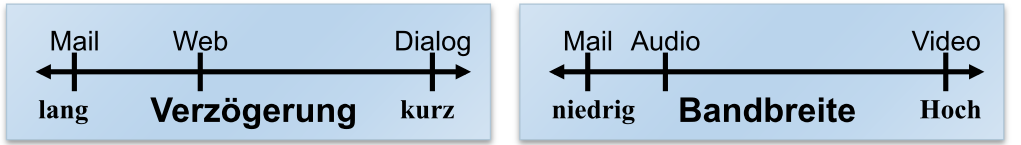
\includegraphics[width=15cm]{img/prio.png}
\end{center}

\subsection{Strategien}
Für jedes Interface sind verschiedene Strategien möglich. 	
\subsubsection{FIFO (First In First Out) Queuing}
	\begin{itemize}
	\item Abarbeitung nach der Reihenfolge des Eintreffens
	\item Vorteil: Einfach zu implementieren und zu modellieren
	\item Nachteile:
		\begin{itemize}
		\item Nur eine Serviceklasse möglich, erlaubt keinerlei QoS. 
		\item Keine Priorisierung von Paketen gegenüber anderen. 
		\end{itemize}
	\end{itemize}

\subsubsection{Weighted Fair Queuing (WFQ)}
	\begin{itemize}
	\item Mehrere Queues mit fairem Multiplexing
	\item Aufteilen der Bandbreite nach Gewichtung. 
	\item Keine Queue „verhungert“,  weil die anderen Queues eine hohe Last haben. 
	\item Bewertung
		\begin{itemize}
		\item Korrekte Zuordnung von Gewichten ist oft schwierig.  
		\item Datenstrom soll nicht höhere Gewichtung anfordern können als erforderlich.
		\item Keine \glqq Leer-Reservation\grqq – sobald eine Queue leer wird, wird dessen Bandbreite für die anderen Queues genutzt. 
		\end{itemize}
	\end{itemize}
\subsubsection{Priority Queuing - Prioritätswarteschlangen}
	\begin{itemize}
	\item Mehrere Queues mit Priorisierung
	\item Zuweisung der gesamten Bandbreite an jeweils höchstpriorisierte Queue (bis diese leer ist)
	\item Wichtiger Verkehr erhält stets genügend Bandbreite, kann allerdings hierdurch weniger wichtigen Verkehr (dauerhaft) blockieren. 
	\item Ermöglichen die Bevorzugung einzelner Übertragungen
	\item Weniger wichtige Übertragungen werden eventuell verdrängt
	\item Bewertung
		\begin{itemize}
		\item Einfach zu implementieren
		\item Die Blockierung weniger wichtigen Verkehrs kann problematisch sein.
		\item Verfahren ist sinnvoll, wenn höchstpriorisierter Verkehr die geringste Datenmenge anliefert und die zugehörige Queue immer wieder geleert wird.
		\end{itemize}
	\end{itemize}
\subsubsection{Custom / Class Based Queuing (CBQ)}
	\begin{itemize}
	\item Mehrere Queues mit unterschiedlichen Prioritäten. 
	\item Datagramme werden entsprechend ihrer Priorität / TOS in die Queues eingereiht. 
	\item Benutzer gibt explizit die Aufteilung der Bandbreite an. 
	\item Angabe als Anzahl Bytes, die zu übertragen sind, bevor die 
	nächste Queue gewechselt wird (transmission window size). 
	\end{itemize}
\subsubsection{Random Early Detection / Discard (RED)}
	\begin{itemize}
	\item Lässt  an bestimmten Punkten im Netzwerk wird überwacht (bspw. zentraler Router). 
	\item RED wurde hauptsächlich für TCP-Anwendungen entwickelt. 
	\item Funktionsweise
		\begin{itemize}
		\item Zufällig werden Pakete verworfen, wenn Überlast auftritt.
		\item Dabei werden Pakete aller Verbindungen gleichermaßen verworfen, damit nicht einzelne Verbindungen \glqq absterben\grqq. 
		\end{itemize}
	\item Absenderknoten erkennen verworfenen Pakete 
		\begin{itemize}
			\item TCP reduziert Window Size wenn die Verbindungsqualität schlechter wird. 
			\item Dann wird schrittweise die Datenrate erhöht, bis wieder Überlast auftritt. 
		\end{itemize}
	\end{itemize}
	
\subsection{QoS Ablauf}	
\begin{center}
	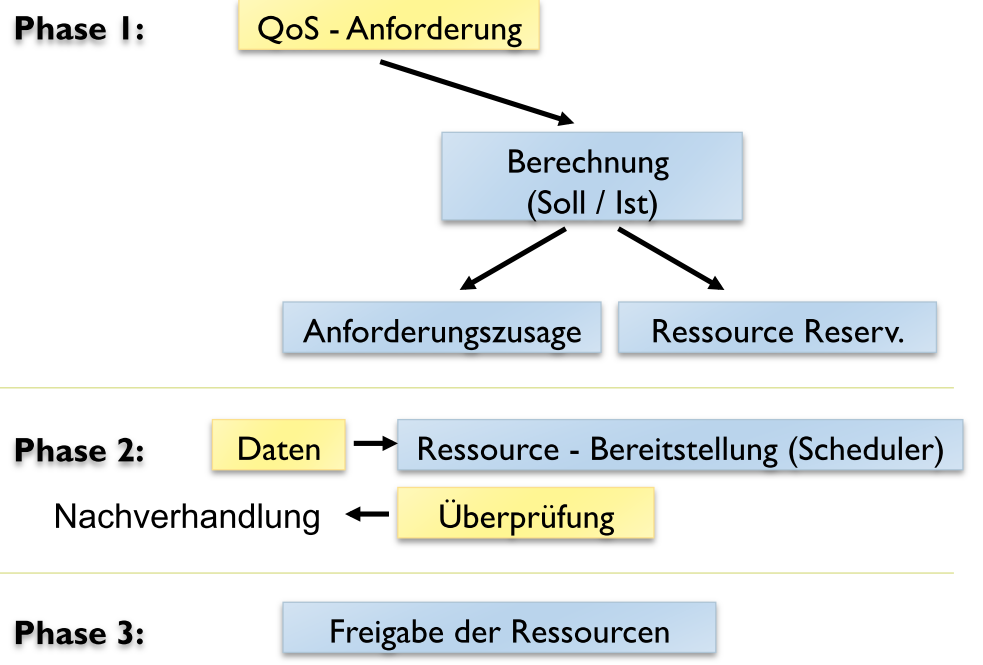
\includegraphics[width=10cm]{img/QoSAblauf.png}
\end{center}
% 140

\section{Multicast}
\label{sec:muliticast}
Multicasts stellen höhere Anforderungen an Router und es sind zusätzliche Protokolle notwendig.
\subsection{Motivation}
Mulitcasts bieten sich dann an, wenn es das Ziel ist, mit so geringem Aufwand wie möglich so viel wie möglich Beteiligte zu erreichen. Wenn es bspw. das Ziel ist, dass mehrere Hörer ein Radioprogramm empfangen gibt es zwei Möglichkeiten:
	\begin{itemize}
	\item Möglichkeit A – Daten werden für jeden Empfänger einzeln geschickt. 
	\item Möglichkeit B – Daten werden möglichst weit nur einmal übertragen und dort, wo sie unterschiedliche Wege gehen müssen, werden sie vervielfacht und verteilt. 
	\end{itemize}
Multicasts können als  Möglichkeit zum Sparen von Bandbreite durch Zusammenfassen von Datenübertragungen betrachtet werden.
	\begin{center}
		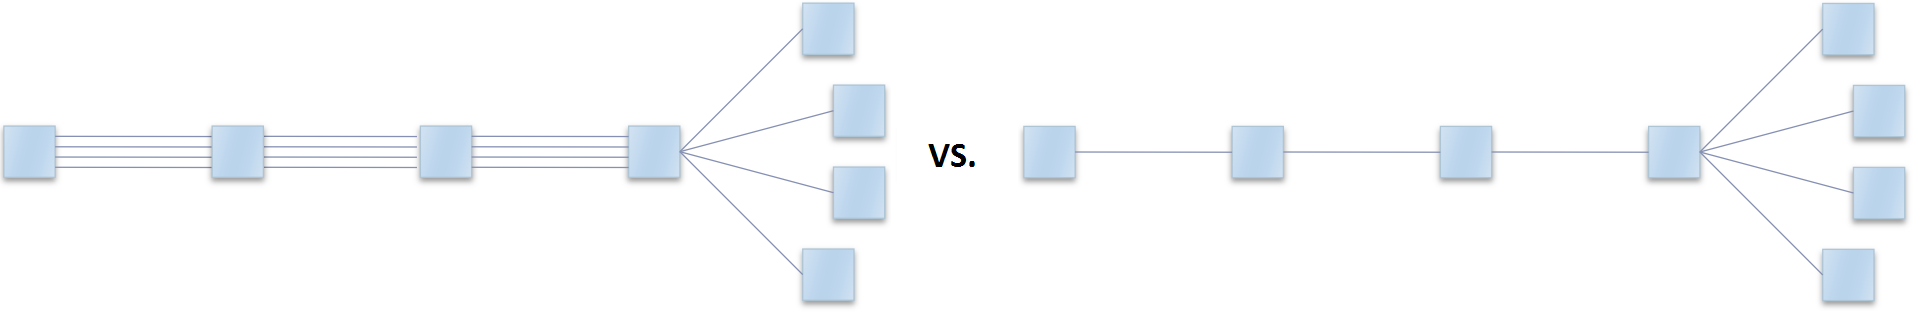
\includegraphics[width=17cm]{img/multicast.png}
	\end{center}

\subsection{Voraussetzungen}
	\begin{itemize}
	\item Für Multicasts werden spezielle \textbf{Router und Routing-Protokolle} benötigt. Diese werden wie üblich durch Berechnung eines Spannbaumes ermittelt. Es kann problematisch werden, wenn mehrere Sender an die Gruppe senden.
	\item Es ist notwendig die \textbf{Gruppenzugehörigkeit} zu übermitteln. Dazu sind spezielle Protokolle notwendig. Ein Rechner, der sich bei einer Gruppe an- oder abmelden mlchte, teilt dies nur seinem lokalen Router mit. Es wird nur die Gruppenadresse übergeben (keine weiteren Informationen). Anschließend muss der Router sich selbst darum kümmern, woher er die Multicastdaten im Internet bekommt. 
	\item Es findet eine angepasste Flusskontrolle statt. In der Regel erfolgt keine Neuübertragung bei negativen Bestätigungen. Außerdem ist eine positive Bestätigungen unpraktikabel.
	\end{itemize}

\subsection{Komplexeres Multicast-Routing}
Zu komplexeren Formen des Multicastings kann es kommen, wenn mehrere Sender existieren:
	\begin{center}
		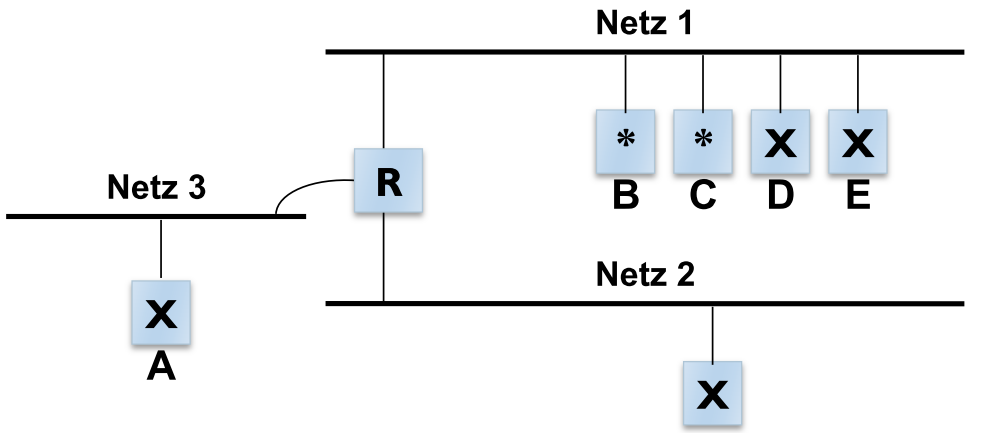
\includegraphics[width=17cm]{img/komplMultiCast.png}
	\end{center}
	\begin{itemize}
	\item Sendet A an die Gruppe X, muss Paket in die Netze 1 und 2 weitergeleitet werden. 
	\item Sendet B an die Gruppe X, muss das Paket in die Netze 2 und 3 weitergeleitet werden. 
	\end{itemize}

\subsection{IGMP}
IGMP (Internet Group Management Protocol) ist ein Protokoll zur Steuerung von Multicast-Gruppen. IGMP ist im RFC 3376\cite{rfc3376} in der aktuellen Version 3 beschrieben. Mit Hilfe von IGMP teilen Hosts und Router dem Multicast-Router ihre Mitgliedschaft in Multicast-Gruppen mit. Außerdem fragen Router in \glqq ihren\grqq Netzen nach Gruppenmitgliedern.
\subsection{Ablauf}
	\begin{itemize}
	\item Router sendet allgemeine IGMP Query an seine Interfaces. Zu Beginn ist jeder Router anfangs Querier. Entdeckt ein Router einen Querier mit niedrigerer IP-Adresse, so wird der Router mit der höheren IP-Adresse zum Non-Querier.
	\item Empfängt ein Host eine Query, startet er einen Timer mit zufälligem Interval zwischen 0 und dem vom Querier vorgegebenen Maximum für jede Gruppe, in der er Mitglied ist. 
	\item Wenn einer Timer abgelaufen ist, sendet der Host einen Report mit TTL=1 an die Gruppe. 
	\item Andere Hosts senden dann keine weiteren Reports, da der Router dieses Interface (Netz) bereits \glqq versorgen\grqq wird.
	\item Empfängt ein Router einen Report, startet er einen Timer für die jeweilige Gruppe. 
	\item Erneute Reports starten den Timer neu. 
	\item Solange der Timer nicht abläuft, bleibt die 	Gruppenmitgliedschaft für das jeweilige Interface erhalten. 
	\item Hosts sollen Anfangs Reports ohne Query senden, um sofort die Mitgliedschaft anzuzeigen. 
	\end{itemize}
 
\begin{figure}[ht]
	\centering
  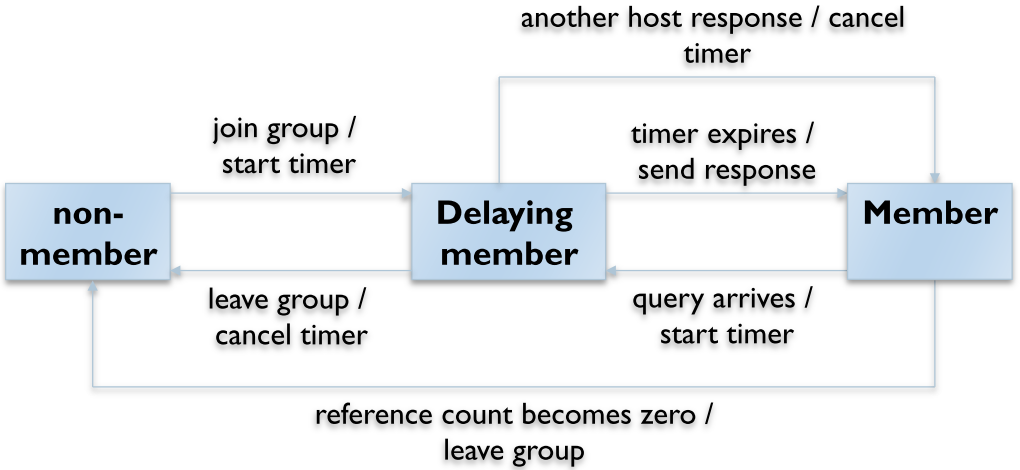
\includegraphics[width=14cm]{img/igmp.png}
	\caption{IGMP Ablauf (vollständig für v.1)}
\end{figure}

\subsection{Nachrichten}
\textbf{IGMP v.1}
	\begin{itemize}
	\item Kennt lediglich die Abonnierung einer Gruppe. 
	\item Membership Reports. 
	\end{itemize}
\textbf{IGMP v.2}
	\begin{itemize}
	\item Explizites Verlassen der Gruppe möglich.
	\item Leave
	\end{itemize}
\textbf{IGMP v.3}
	\begin{itemize}
	\item Quelle der Multicasts kann angegeben werden. 
	\end{itemize}		
	
\subsection{Paketaufbau}
\subsubsection{Membership Query}
	\begin{center}
		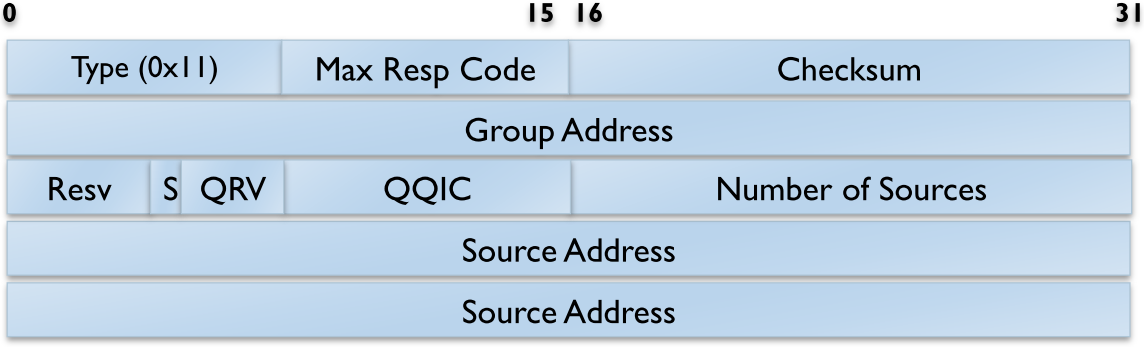
\includegraphics[width=14cm]{img/igmpMQP.png}
	\end{center}
	\begin{description}
	\item[Max Resp Code] Maximum der zufällig zu wählenden Zeit in Zehntelsekunden, bevor ein Report gesendet werden muss. 
	\item[Group Address] Multicast-Gruppe, auf die sich die Query bezieht. 0, falls es eine allgemeine Query ist. 
	\item[S] Flag, das den Multicast-Router auffordert, seinen Timer für Queries nicht neu zu starten.
	\item[QQIC] \glqq Querier's Query Interval Code\grqq - Zeit, nach der der Multicast-Router eine Query absendet. Wird verwendet, um festzustellen, ob der aktuelle Querier im Netz noch aktiv ist. 	
	\end{description}
\subsubsection{Membership Reports}
In Version 3 wird dieses Paket an 224.0.0.22 oder an die entsprechende Multicast-Gruppe gesendet.
	\begin{center}
		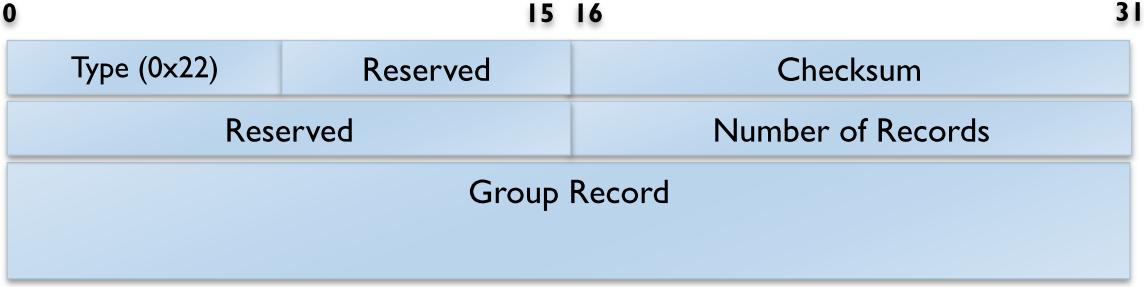
\includegraphics[width=14cm]{img/igmpMRP.png}
	\end{center}
Dabeu enthält der \textbf{Group Record} nähere Informationen zum Report. Insbesondere die Information, ob eine Gruppenmitgliedschaft noch erwünscht ist. 
	\begin{center}
		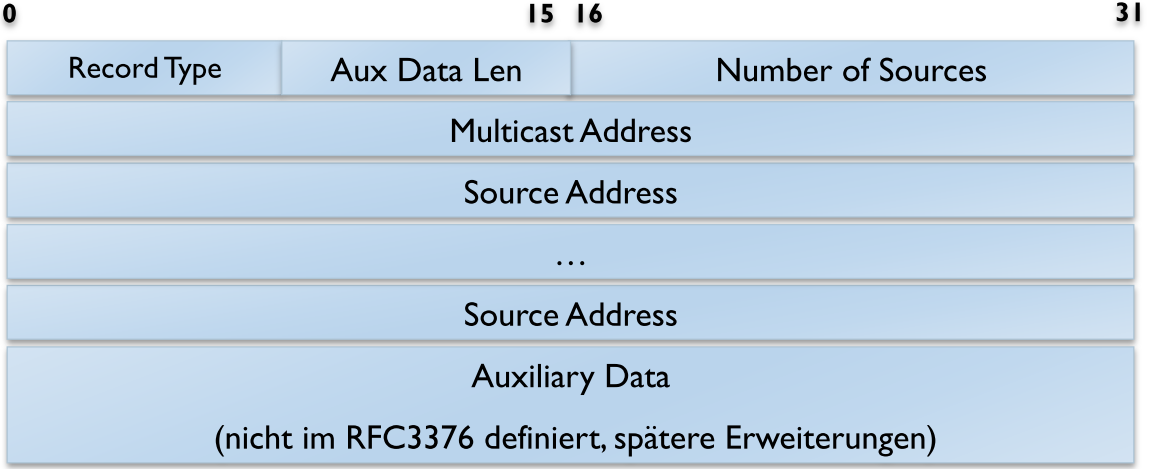
\includegraphics[width=14cm]{img/igmpGR.png}
	\end{center}
	\begin{description}
	\item[RecordType] Umgang mit empfangenen Source Adresse (Multicasts nachfolgender Source Adressen werden empfangen/ignoriert; Hinzufügen/Entfernen von akzeptierten Source Adressen)
	\item[Source Address] ist ein gültiger Absender eines Multicasts
	\end{description}
\subsection{Multicasts und Switches}
Ein Switch  muss Multicasts an alle Mitglieder der Gruppe weiterleiten. Ein regulärer Switch müsste Multicasts wie Broadcasts behandeln. Um die Netzlast zu reduzieren, wird eine Technik namens \textbf{IGMP Snooping} angewendet. 
	\begin{itemize}
	\item Der Switch belauscht (snoop - schnüffeln) den IGMP-Traffic an seinen Ports.
	\item Switch empfängt IGMP Membership Reports (Pakete auf Layer 3). 
	\item Switch fügt den Port (im Sinne von Steckdose) zur Multicast-Gruppe hinzu. 
	\item Nur Ports die einer Multicast-Gruppe beigetreten sind (join) werden in die Forwarding-Table für diese Multicast-Adresse eingetragen. Ports die die Gruppe verlassen (leave) werden aus der Tabelle gelöscht.
	\end{itemize}
	
\subsection{Multicast-Adressen}
%PRÜFEN Klärt das Christians Frage "Was will er uns mit Folie 16 aus 180 sagen??"
% 150, 180
Auf der Vermittlungsschicht werden \textbf{Class-D-IP-Adressen} verwendet.
Diese beginnen mit der Bitfolge \texttt{1110}, die Teilmenge \texttt{224.0.0.0/24} ist für Multicast in lokalen Netzen verfügbar\footnote{Es wird kein Routing-Protokoll benötigt\cite{tanenbaum2003computer}}.
Jede Adresse stellt dabei eine Multicast-Gruppe dar, folglich sind $2^{28} \approx 250$ Mio. Gruppen möglich.

Bei lokaler Kommunikation via Ethernet werden besondere \textbf{Multicast-MAC-Adressen} verwendet.
Diese beginnen mit der festen Bytefolge \texttt{01005E} (3 Byte).
Das vierte Byte beginnt mit dem Bit \texttt{0}.
Die übrigen 23 Bit werden von den 23 untersten Bits der Multicast-Adresse übernommen.
5 Bits aus der Multicast-Gruppe können dabei nicht im Ethernet-Frame abgebildet werden.
\begin{figure}[ht]
	\centering
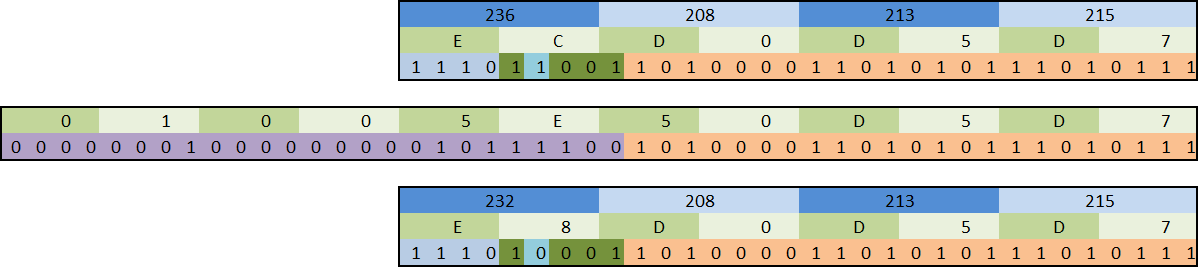
\includegraphics[width=15cm]{img/multicast_adressen}
\caption{Die Multicast-Adressen 236.208.213.215 und 232.208.213.215 werden auf dieselbe Mac-Adresse abgebildet.}
\end{figure}
\section{Zeitsynchronisation}
% 160, 190

\subsection{Notwendigkeit der Zeitsynchronisation}
Authentisierungsverfahren müssen die Gültigkeit von Schlüsseln überprüfen können.
Ebenso haben einige Abläufe eine beschränkte zeitliche Dauer.
Andere Verfahren benötigen Time-Stamps, Vorher-Nachher-Beziehungen von Ereignissen müssen bekannt sein.

Uhren in verteilten Systemen sind nicht zwangsweise synchron.
Sie können unterschiedliche Zeiten aufweisen, je nach Art der Uhr \emph{ticken} sie unterschiedlich schnell (Quarzuhr, Atomuhr).
Zusätzlich kann die physikalische Umgebung diesen Effekt verstärken (z.B. Temperatur einer Quarzuhr).
Eigenschaften von Uhren nach Mühl sind: Drift, Auflösung und Abweichung (von der Realzeit).

\subsection{Logische Zeit}
Manchmal reicht es, nicht den genauen Zeitpunkt von Ereignissen, sondern lediglich die Vorher-Nachher-Beziehung zu kennen.
Man spricht von \textbf{Lamport-Zeitstempel} oder \textbf{Vektoruhren}.
Empfangene Lamport-Zeitstempel werden einfach bei jedem Kommunikationsschritt um eins inkrementiert und dann als eigener Zeitstempel versendet.
Bei der Vektor-Zeit werden zusätzlich die Zeitstempel der anderen Kommunikationspartner mitgeführt.
Dies hat den Vorteil, dass ein kausaler Zusammenhang immer erkennbar ist.

\subsection{Herausforderungen}
\begin{itemize}
	\item Logische Zeitstempel (Lamport-Zeitstempel und Vektor-Zeit) genügen den Anforderungen nicht immer.
	\item Viele Uhren müssen synchronisiert werden.
	\item Die Übertragung eines Zeitstempels kostet Zeit – Latenz.
	\item Die Latenz ist nicht konstant – Jitter.
	\item Die Latenz ist nicht symmetrisch.
\end{itemize}

\subsection{Algorithmen}
\textbf{Anforderungen} an Algorithmen sind symmetrische oder bekannte Laufzeiten und eine konstante Latenz.
Letzteres ist in paketvermittelnden Netzen nicht erreichbar.
\subsubsection{Algorithmus von Cristian}
Clients fragen beim Server nach der korrekten Zeit.
Server kennt die Zeit aus zuverlässiger, externer Quelle.

\subsubsection{Berkeley-Algorithmus}
Server fragt alle verfügbaren Clients nach der Zeit und bildet den Mittelwert.
Zeit wird anschließend an Clients verbreitet.

\subsubsection{Marzullo's Algorithmus}
Versucht den Einfluss des Jitters durch mehrfache Messungen zu eliminieren.
Messungen werden solange durchgeführt, bis das Konfidenzinterval den Anforderungen entspricht.

\subsection{NTP}
NTP\cite{rfc1305, rfc5905} verwendet Marzullo's Algorithmus.
Es löste den ICMP Timestamp Request (Abschnitt \ref{subsec:icmptime}) ab und ist mittlerweile in Version 4 aktuell.
NTP-Server lauschen auf UDP-Port 123.
Im Internet sind Genauigkeiten von $\leq 10ms$ erreichbar.

\subsubsection{Paketaufbau}
\textbf{Anmerkung}: Paketaufbau von Version 4 scheint sich recht stark von Version 3 zu unterscheiden.
Ich bleibe bei der in der Vorlesung besprochenen Version 3.
\begin{description}
	\item[Leap Indicator]: Gibt an, ob Schaltsekunde in dieser Minute hinzugefügt oder entfernt wird  (2 Bit)
	\item[Status]: Gibt mögiche Fehler an.
		\begin{enumerate}
			\setcounter{enumi}{-1}
			\item clock operating correctly
			\item carrier loss
			\item synch loss
			\item format error
			\item interface (Type 1) or link (Type 2) failure
		\end{enumerate}
	\item[Type]: Typ\footnote{Neuere Versionen bezeichnen dies als Stratum; Es gibt quasi eine Hierarchie bei den (Genauigkeiten der) NTP-Server} der Referenzuhr: 1 | Primärreferenz (z.B. Atomuhr) bis 4 | \emph{Eyeball and wrist watch}
	\item[Precision]: Angabe der Genauigkeit der Uhr (als Exponent zur Basis 2)
	\item[Estimated Error]: Geschätzter Fehler zum Zeitpunkt der Synchronisation in Sekunden.
	\item[Estimated Drift Rate]: Geschätzte Drift der Uhr (ohne Einheit).
	\item[Reference Timestamp]: Zeit, auf den die Uhr bei der letzten Synchronisation eingestellt
	wurde.
	\item[Originate Timestamp]: Zeit beim Senden des Pakets
	\item[Receive Timestamp]: Lokale Zeit bei Ankunft des Pakets
	\item[Transmit Timestamp]: Lokale Zeit beim Senden der Anwort
\end{description}

\subsection{SNTP}
Vereinfachung von NTP, bei der auf eine Wiederholung der Zeitsynchronisation verzichtet wird.
So sind etwa Synchronisationen über Multi- und Broadcasts möglich.
Es werden dasselbe Nachrichtenformat und derselbe UDP-Port, wie bei NTP genutzt\cite{rfc4330}.

\subsection{ICMP - Timestamp Request und Reply}
\label{subsec:icmptime}

Timestamp Request\cite{rfc792} ermöglicht die Anfrage eines anderen Systems nach der aktuellen Zeit.
Es handelt sich um ICMP-Nachrichten mit den Type-Werten 13 (Request) oder 14 (Reply)\footnote{Skript sagt hier 17 und 18, im RFC stehen allerdings 13 und 14. Habe Thomas drauf hingewiesen.}.
Empfohlener Rückgabewert sind die Millisekunden seit Mitternacht (Coordinated Universal Time - UTC).
ICMP-Data-Bereich kennt Felder \textbf{Originate Timestamp}, \textbf{Receive Timestamp} und \textbf{Transmit Timestamp} (je 32 Bit); diese scheinen dieselbe Bedeutung wie bei NTP zu haben.
Außerdem \textbf{Identifier} und \textbf{Sequence Number}, diese gestatten dem Sender eine Zuordnung von Replies bei mehreren Requests.
Letztere werden vom Sender eingetragen und vom Empfänger in die Antwort kopiert.

\section{Internet Control Message Protocol}

ICMP ist ein Layer-3-Protokoll zur Steuerung des Nachrichtenaustausches im Internet\cite{rfc792}\footnote{Laut Folien RFC 950\cite{rfc950}, aber das ist Quatsch (\emph{Internet Standard Subnetting Procedure})}.
Es dient häuptsächlich dem Austausch von Status- und Fehlermeldungen zwischen Gateways und Hosts.
Die Nachrichten werden über IP-Datagramme übertragen, das Protokoll ist verbindungslos.

\subsection{Paketaufbau}
Eine ICMP-Nachricht besteht aus den Feldern \textbf{Type}, \textbf{Code}, \textbf{Checksum} und \textbf{Data}, angeführt von einem 20 Byte IP-Header.
Der IP-Header hat häufig vorbestimmte Feldwerte, z.B. Type of Service = 0, weitere Infos im RFC.

\begin{description}
	\item[Type]: Bestimmt das Format der weiteren  Felder. (1 Byte)
	\item[Code]: Inhalt Abhängig vom Type (1 Byte)
	\item[Checksum]: Prüfsumme\footnote{Scheinbar abhängig vom Type; häufig: \emph{The checksum is the 16-bit ones's complement of the one's complement sum of the ICMP message starting with the ICMP Type.}} (2 Byte) 
	\item[Data]: Nicht immer genutzt; Enthält beispielsweise bei Type \emph{Redirect Message} (5) die \emph{Gateway Internet Address} oder die in Abschnitt \ref{subsec:icmptime} beschriebenen Felder für Timestamps.
\end{description}

\subsection{Beispiele}
Im Skript existiert eine umfangreiche Tabelle von Funktionen und entsprechender Werte für Type- und Code-Felder.
Diese auswendig zu lernen entspräche nicht 80-20.
Daher beschränke ich mich hier nur auf zwei Beispiele (+ Zeitsynchronisation in Abschnitt \ref{subsec:icmptime})

\subsubsection{Destination Unreachable}
Wird beispielsweise gesendet, wenn er Empfänger laut den Routing-Tabellen eines Gateways nicht erreichbar ist, z.B. weil die Distanz zum Zielnetzwerk unendlich ist.
Empfänger im IP-Header ist der ursprüngliche Absender einer (nicht zustellbaren) Nachricht.
Der ICMP-\textbf{Type} ist 3, der Code gibt genauere Informationen zur Fehlerursache (z.B. 3 | port unreachable)
\subsubsection{Ping}
Beispiel nicht aus dem Skript.
Beim Request wird ein \textbf{Echo-Request} (Type 8) versendet.
Das Feld \textbf{Code} enthält den Wert 0\footnote{Laut RFC scheint die Möglichkeit zu bestehen, dass hier etwas anderes steht. Warum das so ist, kann ich allerdings nicht finden}.
\textbf{Identifier} und \textbf{Sequence Number} helfen bei Unterscheidung mehrerer Requests/Replys.
Im \textbf{Data} Feld kann scheinbar noch unbestimmter Payload mitgesendet werden.

Bei der Antwort werden Sender- und Empfängeradresse im IP-Header vertauscht.
Der \textbf{Type} ist 0 (Echo-Reply).
Weitere Felder werden aus dem Request übernommen.

\subsection{Regeln}
ICMP-Fehler-Nachrichten werden nie als Folge auf
\begin{itemize}
\item  eine ICMP Fehlermeldung („Teufelskreislauf“) erzeugt.
\item  ein Datagram, das an eine IP Broadcast Adresse oder eine IP
Multicast - Adresse (class D) gesendet wird, erzeugt.
\item  ein Datagram, welches als Link - Layer Broadcast gesendet
wird, erzeugt.
\item  ein anderes Fragment als des ersten erzeugt.
\item  ein Paket erzeugt, dessen Quelladresse nicht einen einzelnen Host definiert.
\end{itemize}


\section{Internet Group Message Protocol}
%TODO Ist in Mitschriften genannt worden

\section{Voice over IP}
% 200, 210
VoIP ist kostengünstig, da taugliche IP-Geräte verbreitet und auf Grund der hohen Stückzahlen billig zu produzieren sind. Außerdem sind die Betriebskosten gering.\\
Des Weiteren gibt es eine Vielzahl an Gründen für VoIP: 
\begin{itemize}
	\item Integration von Sprach- und Datendiensten.
	\item Leichtere Implementierung komplexerer Anwendungen	(z.B. Call Center).
	\item Potentiell geringerer Bandbreitenbedarf.
	\item Verfügbarkeit von IP-Netzen.
\end{itemize}
Wichtige Aspekte sind die Digitalisierung der Sprache (Bandbreite, Gesprächsqualität) und die eigentliche Übertragung der Sprache (Quality of Service / Priorisierung).
\subsection{Digitalisierung}
Zur Digitalisierung der Sprache bestehen verschiedene Möglichkeiten:
\begin{itemize}
	\item Zählverfahren - „Hochzählen“ um jeweils einen Spannungsschritt und Vergleichen mit dem Input.
	\item Sukzessive Approximation – schrittweise Annäherung der Spannung entsprechend der Bitwertigkeit mittels D-A-Wandler	und Vergleich (Komperator).
	\item Parallel-Umsetzer – ein Komperator pro möglichem	Eingangswert.	
\end{itemize}
Die Digitalisierung erfolgt mittels Quantisierung. Durch begrenzte Auflösung des A-D-Wandlers kommt es zu einem Quantisierungsrauschen. Dadurch entstehen Quantisierungsfehler:\\
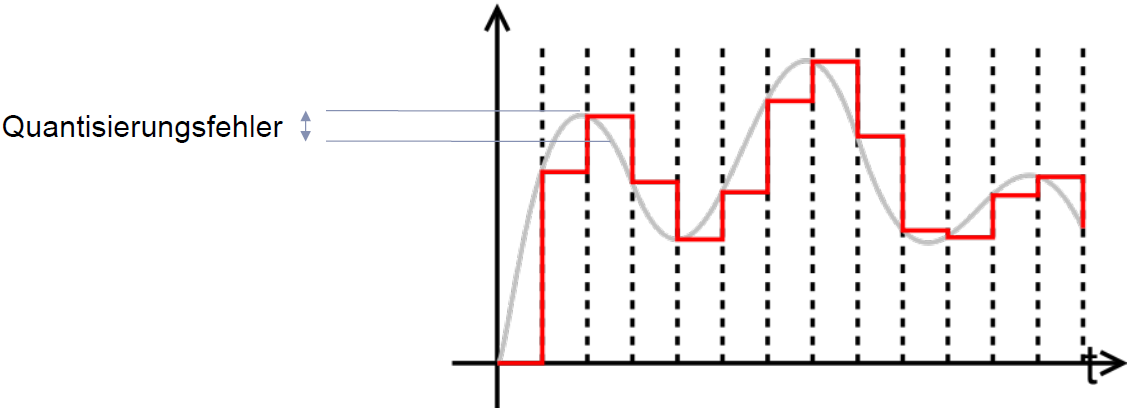
\includegraphics[width=12cm]{img/quantisierungsfehler.png}
\subsection{Sprachqualität}
Eine Aussage über die subjektive Sprachqualität wird in der Regel über \glqq Testhörer\grqq getroffen. Andere Methoden vergleichen das Eingangs- und das Ausgangssignal algorithmisch, z.B. Perceptual Speech Quality Measurement.\\
Die Sprachqualität hängt von verschiedenen Faktoren ab:
\begin{itemize}
	\item Latenz\\
	(ITU-T G.114 empfiehlt maximal 300ms, andere Empfehlungen unter 150ms.)
	\item Jitter
	\item Packet Loss
	\item Quantisierung
	\item Abtastfrequenz
	\item Art der Sprachkodierung
\end{itemize}
Die Sprachqualität wird in MOS (Mean Opinion Score) angegeben.
\subsection{Sprachkodierung}
Die folgenden Kodierungen können durch verschiedene \glqq Trick\grqq verbessert werden:
\begin{itemize}
	\item Silence Detection (auch Abschaltung des Senders DTX bei GSM).
	\item Comfort Noice (teilweise mit unterschiedlichen Rauschmodellen).
	\item Ein Problem bei der Mehrfachkodierung ist, dass falls mehrfach der Codec gewechselt wird, die
	Sprachqualität stark abnimmt (z.B. bei Netzübergängen).
\end{itemize}
\subsubsection{Pulse Code Modulation (PCM)}
\begin{itemize}
	\item Waveform Codec - Abtastung und Erzeugung unkomprimierter, unveränderter Daten.
	\item PCM ist ein Pulsmodulationverfahren, das ein zeit- und wertkontinuierliches analoges Signal in ein zeit- und wertdiskretes digitales Signal umsetzt.
	\item G.711 zum Beispiel mit 8000Hz, 8bit (64kbit/s netto)
	\item Funktionsweise:
	\begin{enumerate}
		\item Abtastung des analogen Signals mit einer zeitlich konstanten Abtastrate. Dabei wird aus dem zeitkontinuierlichen Signalverlauf eine zeitdiskrete Signalfolge gebildet. Zur Erhaltung der Information in der zeitdiskreten Folge ist die Erfüllung des Nyquist-Shannon-Abtasttheorems notwendig. Dies bedeutet, dass die Abtastrate mehr als doppelt so groß sein muss, wie die im Signalverlauf höchste vorkommende Frequenzkomponente ist.
		\item Quantisierung auf diskrete Werte mit endlich vielen Stellen.
		\item Erzeugung des Digitalsignals mittels Codierung.
	\end{enumerate}
\end{itemize}
\subsubsection{Differential Pulse Code Modulation (DPCM)}
\begin{itemize}
	\item Die Kodierung wird teilweise auch Delta PCM genannt und es handelt sich um einen Waveform Codec.
	\item Wegen der relativ langsamen Änderungen des Eingangssignals lassen sich einige Werte mit annehmbarer Genauigkeit	vorhersagen.
	\item DPCM überträgt Differenz zwischen Sample n und Sample n+1.
	\item Bei einigen Varianten von DPCM werden lediglich die Differenzen zwischen einer Vorhersage und Messwert übertragen.
	\item Gleicher Informationsgehalt, wie PCM, allerdings reduzierte Datenübertragung.
\end{itemize}
\subsubsection{Adaptive Differential Pulse Code Modulation (ADPCM)}
\begin{itemize}
	\item Wie DPCM, allerdings mit dynamischer Anpassung der Quantisierungsschritte.
	\item Verlustbehaftet
	\item G.726 mit 32kbit/s hat MOS von 4,0.
\end{itemize}
\subsubsection{Vocoder}
\begin{itemize}
	\item Einige Codecs versuchen, ein mathematisches Modell der an der Spracherzeugung beteiligten Vokaltrakts zu erstellen.
	\item Es werden die \glqq Einstellungen\grqq des Vokaltrakts übertragen.
	\item Es ist jedoch keine natürlich klingende Ausgabe möglich.
\end{itemize}
\subsubsection{Hybride Codecs}
\begin{itemize}
	\item Hybride Codecs kombinieren beide Varianten und benutzen Teilinformationen aus Waveform Codecs und von Vocodern.
	\item Erzeugen immer kleine Verzögerung durch blockweise Bearbeitung der Daten.
	\item G.728 – Low Delay Code-Excited Linear Predictive, MOS 3,9	bei 16kbit/s.
	\item G.723 – Algebraic Code-Excited Linear Prediction – 30ms Verzögerung.
	\item GSM-Codec.
\end{itemize}

\begin{center}
	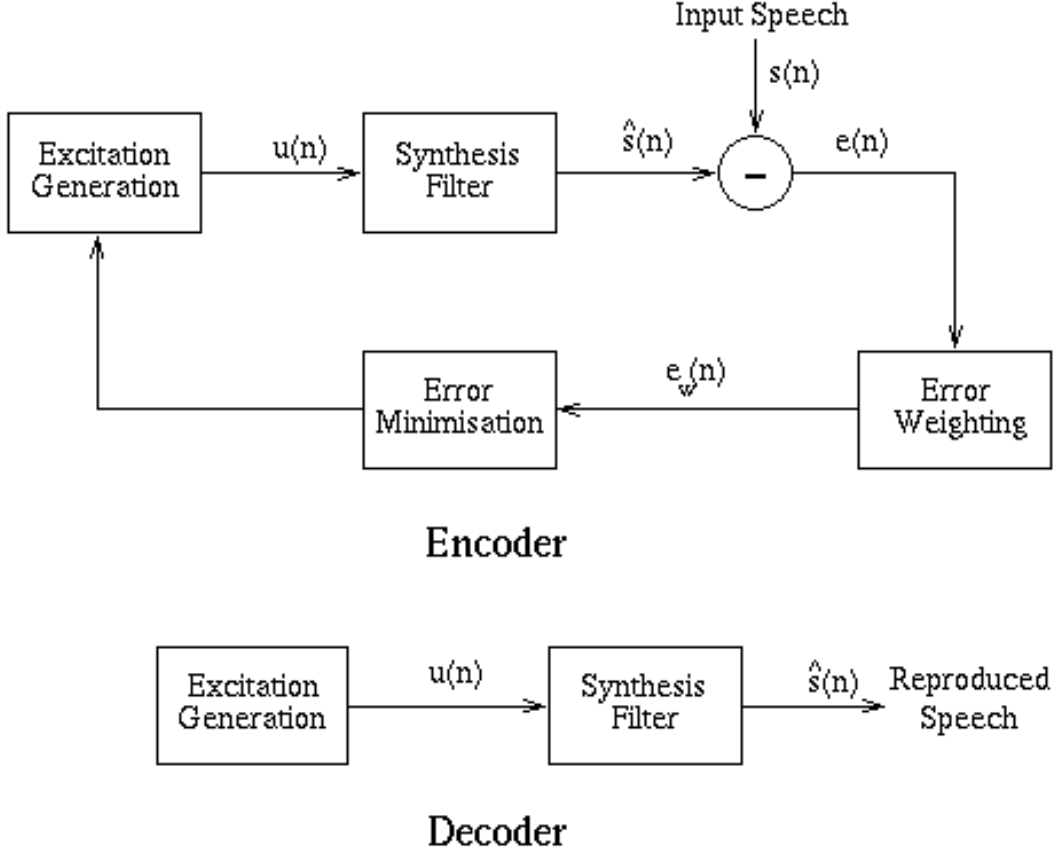
\includegraphics[width=10cm]{img/hybridVoIP.png}
\end{center}
\subsection{Aufbau eines VoIP-Systems}
Es ist notwendig, dass neben dem Austausch der reinen Sprachdaten (oder Audio-Video-Daten) eine Möglichkeit zur Steuerung besteht. Die folgenden Punkte sind dabei zu beachten:
\begin{itemize}
	\item Gesprächsauf- / -abbau.
	\item Umleitungen.
	\item Ansagen / Anrufbeantworter.
	\item Konferenzschaltung
	\item Übergang in andere Netze.
	\item Ressourcenverwaltung / QoS-Steuerung.
	\item Abrechnung / Logging / „Vorratsdatenspeicherung“.
\end{itemize}

\subsection{Migration}
Zur Zeit existieren unterschiedliche Telefonnetze, Anbieter und Standards. Deshalb ist eine Umstellung auf VoiIP nicht instantan möglich. Die Umstellung erfordert eine schrittweise Migration: Zeitweiser Parallelbetrieb; Spezielle Telefon-Router zur Kostenoptimierung; Umsetzer zwischen verschiedenen Standards und ein Austausch von Telefonanlagen.

\subsection{RTP}
	\begin{itemize}
	\item RTP (Real Time Transport Protocol) ist ein Protokoll zum Streaming von Daten. 
	\item RTP dient der Übertragung von Daten und optional kann RTCP genutzt werden, um Feedback für QoS zu erhalten.
	\item Basiert auf UDP, Port frei wählbar, default 5004 und 5005. 
	\end{itemize}	
	\begin{center}
		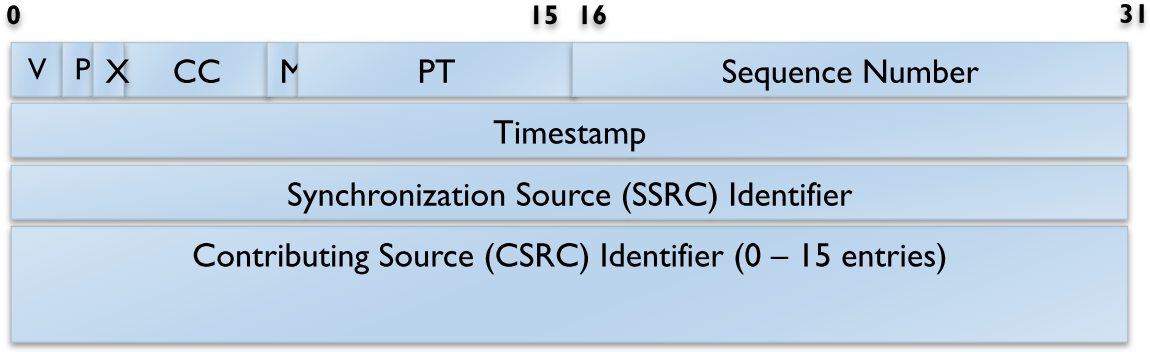
\includegraphics[width=14cm]{img/rtp.png}
	\end{center}
	\begin{description}
	\item[V - Version] 2
	\item[P - Padding] Gibt an, ob an Ende des Datenpakets Padding-Bytes enthalten sind. Falls gesetzt, enthält das letzte Byte im Payload die Anzahl 	der Padding-Bytes. 
	\item[X - Extension] Header-Erweiterung vorhanden.
	\item[CC - SRC-Count] Anzahl der CSRS-Felder
	\item[M – Marker] Verschiedene Einsatzmöglichkeiten, gemäß RFC1890 bspw. 
		\glqq Silence im Datenstrom möglich\grqq. 
	\item[PT – Payload Type] Typ der Daten (G.726-32, GSM, 9 – G.722, QCELP, JPEG Video)
	\item[Timestamp] Zeitpunkt des ersten Samples. 
	\item[Synchronization Source ] Normalerweise der Sender der Nachricht, derjenige, der Timestamps setzt. 
	\item[CSRC] Im Falle, das verschiedene Signale gemischt werden (Mixer, z.B. für Konferenzgespräche), werden die einzelnen Quellen hier aufgeführt. 
	\end{description}
	\begin{itemize}
	\item RTP wird häufig auch als Multicast versendet. RTCP Reports werden dann in der Regel nicht ausgewertet. 
	\end{itemize}
	
\subsection{RTCP}
	\begin{itemize}
	\item das RTCP (RealTime Control Protocol)  definiert verschiedene Kontrollnachrichten. Dabei können mehrere Kontrollnachrichten (RTCP Packets) in einem Compound Packet zusammen versendet werden. 
	\item Sender Report (SR) kann bspw. enthalten:
		\begin{itemize}
			\item NTP Timestamp 
			\item RTP Timestamp 
			\item Fraction Lost (Anteil der verlorenen Pakete seit dem letzten Report) – in n von 256. 
			\item Cumulative Number of Packets Lost 
			\item Interarrival Jitter. 
			\item Last SR Timestamp. 
		\end{itemize}
	\item Receiver Report (RR) enthält bspw. Interarrival Jitter
	\item Source Description (SDES)
	\item BYE
	\item APP (Application Specific Function)
	\end{itemize}

\subsection{Protkolle zur Übertragung von Steuerungsinformationen}	
\subsubsection{SIP}	
	SIP (Session Initiation Protocol)\cite{rfc2543} dient nicht zur Übertragung multimedialer Daten. Das Protokoll steuert den Aufbau einer Verbindung zwischen Kommunikationspartnern. Die Verbindung wird hierbei über HTTP-ähnliche Nachrichten gesteuert.\\
	Dabei beteiligte Entitäten sind:
	\begin{itemize}
	\item Proxy Server 
	\item Redirect Server 
	\item User Agent Server 
	\item Registrar 
	\end{itemize}
	Es kann aus den folgenden Gründen zu Problemen beim Verbindungsaufbau kommen:
	\begin{itemize}
	\item \textbf{Überwinden von NAT Gateways} 
		\begin{itemize}
		\item Nutzer registrieren sich bei Proxy Servern. 
		\item Invitations und Requests werden über Proxy Server weitergeleitet. 
		\item Häufig kennen User Agents ihre IP-Adresse nicht, dann häufig STUN-Server. \\
		\textit{Ein STUN-Server (\textbf{S}imple \textbf{T}raversal of \textbf{U}DP Through \textbf{N}etwork Address Translators [NATs]) ermöglicht es NAT-Clients (z. B. Computern hinter einer Firewall), die Kommunikation mit einem VoIP-Provider außerhalb des lokalen Netzwerks aufzubauen.}
		\end{itemize}
	\item \textbf{Discovery des Kommunikationspartners}
		\begin{itemize}
		\item IP Nummern sind untauglich, da veränderlich. 
		\item Proxy Server enthalten Registrierungsdaten der Nutzer. 
		\end{itemize}
	\end{itemize}
	
\subsubsection{Erinnerung: ASN.1}	
	Die Abstract Syntax Notation One ist eine Beschreibungssprache zur Definition von Datenstrukturen sowie Festlegungen zur Umsetzung von Datenstrukturen und Elementen in ein netzeinheitliches Format.
	\begin{verbatim}
FooProtocol DEFINITIONS ::= BEGIN 
    FooQuestion ::= SEQUENCE { 
        trackingNumber INTEGER, 
        question       IA5String 
    } 
    FooAnswer ::= SEQUENCE { 
        questionNumber INTEGER, 
        answer         BOOLEAN 
    } 
END 
	\end{verbatim}
	
\subsubsection{H.323}	
	\begin{itemize}
	\item Bei H.323 handelt es sich um einen übergeordneter Signalisierungsstandard für Multimedia-Dienste, inkl. VoIP. Die Beschreibung erfolgt in ASN.1.
	\item Der Standard definiert eine Reihe von Protokollen für die Steuerung von multimedialer Kommunikation.
		\begin{description}
		\item[H.225.0] - Registration, Admission, and Status (RAS)
		\item[H.245] -  Steuerung, beschreibt Nachrichten zum Öffnen und Schließen logischer Kanäle für Audio, Video und Daten. 
		\end{description}
	\item Es werden außerdem eigene Codecs definiert (H.261, H.263, H264 - letzterer für HD DVD und Blu-Ray)
	\item H.323 ist Transport-Protokoll-unabhängig
	\end{itemize}
	
\subsubsection{H.225-0 (RAS)}
Definiert eine Reihe von Nachrichten für die Registrierung, Zugangssteuerung und Statusübertragung. \\
(Discovery, Registration, Unregistration, Admission – ARQ (Request) / ACF (Confirm) / ARJ (Reject), Bandwidth Change, Endpoint Location, Disengage, Status)



\section{World Wide Web und HTTP}
% 220, 230
Durchbruch des Internets erfolgte erst nach dem Erscheinen des ersten graphischen WWW-Browsers (\glqq Mosaic\grqq).
Dieser ermöglichte erstmals den komfortablen und effizienten Zugriff auf die Ressourcen des Internets.
Das zuvor \glqq beliebte\grqq{\ }Gopher wurde relativ schnell verdrängt.
Bis zum Ende der 90er-Jahre vervielfachte sich die Zahl der Websites dramatisch (1993 ca. 50; 1994 ca. 800, 2000 über 22 Millionen)

\subsection{Anforderungen an Internet-Protokolle}

\begin{itemize}
	\item Weitestgehende Unabhängigkeit von der Netzwerk-Hardware.
	\begin{itemize}
		\item Übertragungsmedium (Kupferkabel, Lichtwellenleiter usw.)
		\item Typ des lokalen Netzwerks (Ethernet, Token Ring usw.)
	\end{itemize}
	\item Erreichbarkeit aller Rechner im gesamten Internet.
	\item Fehlererkennung und Fehlerkorrektur.
	\item Logische Adressierung (Adresse eines Rechners sollte nicht von der Netzwerk-Hardware abhängen, da bei Defekt einer Ethernet-Karte beispielsweise eine ausgetauschte Karte zu einem Adresswechsel führen würde).
	\item Verbindungsherstellung.
	\item Datenübertragung (Versendung von Datenpaketen /Datagrammen).
\end{itemize}

\subsection{Hypertext Transfer Protocol}
\begin{framed}
\textbf{Anmerkung: } Die Folien sind hier nicht so geil.
Ich schreibe das Interessanteste zu HTTP aus dem Tanenbaum\cite{tanenbaum2003computer} und den Folien hier zusammen, sodass der Leser danach hoffentlich einen kurzen, zusammenhängenden Schnack über das Thema hinbekommt.
\end{framed}

HTTP 1.1 wurde in RFC 2616\cite{rfc2616} definiert und später um  TLS(RFC 2817 \cite{rfc2817}) erweitert; 2014 wurde die gesamte Protokollsuite in den RFCs 7230 - 7235 neu formuliert\cite{rfc7230,rfc7231,rfc7232,rfc7233,rfc7234,rfc7235}.
Es handelt sich um ein\textbf{generisches}\footnote{Es ermöglicht die Übertragung jeglicher Daten und beschränkt sich nicht nur auf Hypertext-Dokumente.}, \textbf{zustandsloses} \textbf{Request-Response-Protokoll}, 
Daten werden im Klartext übermittelt, wenn keine explizite Verschlüsselung gefordert ist.
Ressourcen werden über URIs\cite{rfc2396} adressiert.\footnote{Angeführt durch die Protokollangabe http:// oder https://, dabei handelt es sich dann allerdings um eine URL.}

\subsubsection{Verbindungen}

HTTP nutzt den TCP-Port 80 (bzw 443 für HTTPs).
Während bei HTTP 1.0 für jede Anfrage und Antwort eine eigene Verbindung aufgebaut wurde, bleibt diese in HTTP 1.1 eine Weile erhalten (\emph{persisten connections}).
Auf diese Weise wird der Overhead zum Auf- und Abbau der Verbindung, sowie der Leistungsverlust durch \textbf{TCP-Slow-Start} verringert, wenn weitere Inhalte (z.B. Bilder, CSS, Skripte) in Folge der originalen Anfrage nachgeladen werden.
Hier ist auch \textbf{Pipelining} erlaubt, das heißt, dass mehrere Anfragen gesendet werden können, bevor entsprechende Antworten empfangen wurden.

\subsubsection{Methoden}

HTTP kennt mehrere Methoden\footnote{Laut Tanenbaum\cite{tanenbaum2003computer} scheint hier tatsächlich die Methode aus dem objektorientierten Sprachgebrauch gemeint zu sein.}.
Eine Anfrage beginnt immer mit dem Namen der angeforderten Methode.
Einige Methoden sind:
\begin{description}
	\item[GET]: Lesen einer Website
	\item[HEAD]: Lesen des Headers einer Website, zum Beispiel genutzt von Suchmaschinen
	\item[POST]: Anhängen von Daten an eine Website, beispielsweise genutzt, um Formulardaten an den Server zu übermitteln.
\end{description}
Weitere sind beispielsweise \textbf{PUT}, \textbf{DELETE}, \textbf{TRACE}, \textbf{CONNECT} und \textbf{OPTIONS}.
Eine einfache Anfrage wäre etwa \texttt{GET index.html HTTP/1.1}.
Diese fordert offensichtlich die Datei \texttt{index.html} unter Verwendung von HTTP 1.1 an.

Die Antwort auf eine Anfrage besteht aus einer Statuszeile und gegebenenfalls weiteren Informationen.
Zu Letzterem zählt insbesondere der angeforderte Inhalt, sofern verfügbar.
In der Statuszeile ist ein \textbf{Statuscode}, bestehend aus drei Ziffern zu finden.
Diese Statuscodes werden, entsprechend der ersten Ziffer, in fünf Gruppen geordnet:
\begin{description}
	%OPTIONAL Übersetzen
	\item[1xx]: Informational - Request received, continuing process
	\item[2xx]: Success - The action was successfully received, understood, and accepted
	\item[3xx]: Redirection - Further action must be taken in order to complete the request
	\item[4xx]: Client Error - The request contains bad syntax or cannot be fulfilled
	\item[5xx]: Server Error - The server failed to fulfill an apparently valid request
\end{description}
\textbf{Klugscheißerwissen:} Neuer Statuscode 451 für zensierte Inhalte\cite{http451rfcDraft, sokolov2015http451}
\subsubsection{Header}

An die im letzten Abschnitt gezeigten Anfrage können weitere Informationen in \textbf{Request Headern}\footnote{Möglicherweise eine Sache der Übersetzung, aber im Tanenbaum wird ein Feld als einzelner Header bezeichnet. Ich switche gleich zu Feldern statt Headern.} angefügt werden.
Analog dazu kann die Antwort mit \textbf{Response Headern} versehen werden.
Einige dieser Felder können nur bei Anfragen (z.B. User-Agent), einige nur bei Antworten(z.B. Content-Encoding), einige bei beidem (z.B. Date) übermittelt werden.

Der Client kann beispielsweise in seiner Anfrage angeben, welche Zeichensätze (\emph{Accept-Charset}, z.B. ISO-8859-1) und Codierungen (\emph{Accept-Encoding}, z.B. gzip, compress oder deflate\cite{rfc1950,rfc1951}) er akzeptiert .
Entsprechend enthält die dann Antwort (im Allgemeinen) die Felder \emph{Content-Encoding} und \emph{Content-Type\footnote{Eigentlich für den MIME-Typ, enthält aber auch den charset.}}

%FRAGE will hier noch jemand eine Liste mit weiteren Beispielen?


%\subsubsection{Caching}

%OPTIONAL HTTP Caching optional

\subsection{HTTP/2}

HTTP/2 wird in RFC 7540\cite{rfc7540} definiert.
Es erweitert seinen Vorgänger um einige neue Funktionen:
\begin{itemize}
	\item Möglichkeit des Zusammenfassens mehrerer Anfragen,
	\item Weitergehende Datenkompressionsmöglichkeiten,
	\item Binär kodierte Übertragung von Inhalten und
	\item Server-initiierte Datenübertragungen (push-Verfahren).
\end{itemize}
HTTP/2 überträgt sämtliche Nachrichten in Streams.
Ein Stream ist eine unabhängige, bidirektionale Sequenz von Frames, die zwischen Client und Server in einer HTTP/2 Verbindung übertragen werden. 
Es handelt sich weiterhin um ein Klartext-Protokoll, die Syntax ist hierbei jedoch stark verändert worden.
Es basiert in weiten Teilen von Googles \textbf{SPDY}, welches wiederum auf HTTP aufsetzt und dieses verbessern sollte.
Ziele bei der Entwicklung von SPDY waren unter anderem:
\begin{itemize}
	\item SPDY-Übertragung wird immer mittels TLS verschlüsselt	(HTTP/2 optional, aber Browser-Hersteller verlangen Verschlüsselung)
	\item Multiplexen der Übertragungen
	\item Über eine einzelne TCP-Verbindung können beliebig viele Dokumente parallel übertragen werden
	\item Möglichkeit zur Priorisierung einzelner Anfragen
\end{itemize}

\subsection{File Transfer Protocol}

FTP\cite{rfc959} ist ein Protokoll zum Kopieren von Dateien von einem System auf ein anderes.
Es wurde so konzipiert, dass verschiedene Hosts (betriebssystemunabhängig), Dateitypen (ASCII, binary, etc.) und Dateistrukturen (byte stream oder record oriented) unterstützt werden.
Zum Übertragen der Daten wird in der Regel der TCP-Port 20 verwendet, für Steuernachrichten Port 21.
Der prinzipielle Ablauf ist wie folgt:
\begin{enumerate}
	\item FTP - Clientprozess wird gestartet.
	\item Client baut eine TCP Verbindung zum Server auf.
	\item Durch TCP werden zwischen den beiden Prozessen zwei Verbindungen aufgebaut (Daten und Kommunikation).
	\item Interaktiver Anwender muss Zugangsberechtigung auf Server eingeben (Login/Passwort bzw. anonym).
	\item Datentransfer kann erfolgen (Textdateien und Binärdateien).
\end{enumerate}


\subsubsection{Steuersignale und Return Codes}
Steuersignale werden im Klartext vom Client an den Server gesendet.
%\begin{multicols}{2}
%FRAGE Multicols wieder aktivieren?
\begin{description}
	\item [USER] (User Name) - Eingabe einer UserID für den Server.
	\item [PASS] (Password) - Passwort an den Server senden.
	\item [CWD] (Change Working Directory) - Wechseln des Arbeitsverzeichnisses.
	\item [PORT] - Angabe der Client Callback-Adresse (IP und Port).
	\item [LIST] - Auflisten von Dateien / Verzeichnissen.
	\item [RETR] (Retrieve) - Hole eine Datei vom Server.
	\item [STOR] (Store) - Speichere eine Datei auf dem Server.
	\item [SYST] (System) - Erhalte vom Server den System - Typ.
	\item [TYPE] - Angabe der zu nutzenden Datendarstellung (A / I).
	\item [ABOR] (Abort) - Beendet den Datentransfer bzw. den letzten Befehl.
	\item [QUIT] - Ausloggen vom Server / Verbindung abbauen.
	\item [MKD] (Make Directory)
	\item[RMD] (Remove Directory) 
	\item[DELE] (Delete)
	\item[PWD] (Print Working Directory)
	\item [HELP]
\end{description}
%\end{multicols}

Analog zu den Statuscodes bei HTTP sendet der Server Return Codes.
\begin{description}
\item [1yz] – Positiver Beginn eines Befehls.
\item [2yz] – Positive Beendigung eines Befehls.
\item [3yz] – Positiver Zwischenbericht.
\item [4yz] – Transientes Problem. Der Befehl wurde nicht ausgeführt.
\item [5yz] – Definitives Problem.
\item [x0z] – Syntaxfehler.
\item [x1z] – Allgemeine Information.
\item [x2z] – Verbindungszustand.
\item [x3z] – Authentisierung und Accounting
\item [x4z] – Nicht spezifiziert.
\item [x5z] – Status des Dateisystems.	
\end{description}

\subsubsection{Aktiver und Passiver Modus}

Beim \textbf{aktiven} Modus baut der Client eine den Steuerkanal auf und öffnet einen TCP-Port zur Datenübertagung.
Dieser teilt er dem Server mit, welcher sich darauf verbindet und die Datenübertragung kann beginnen.
Beim \textbf{passiven} Modus teilt der Server dem  Client einen Port mit.
Auf diesen Verbindet er sich dann zur Datenübertragung.

\begin{center}
	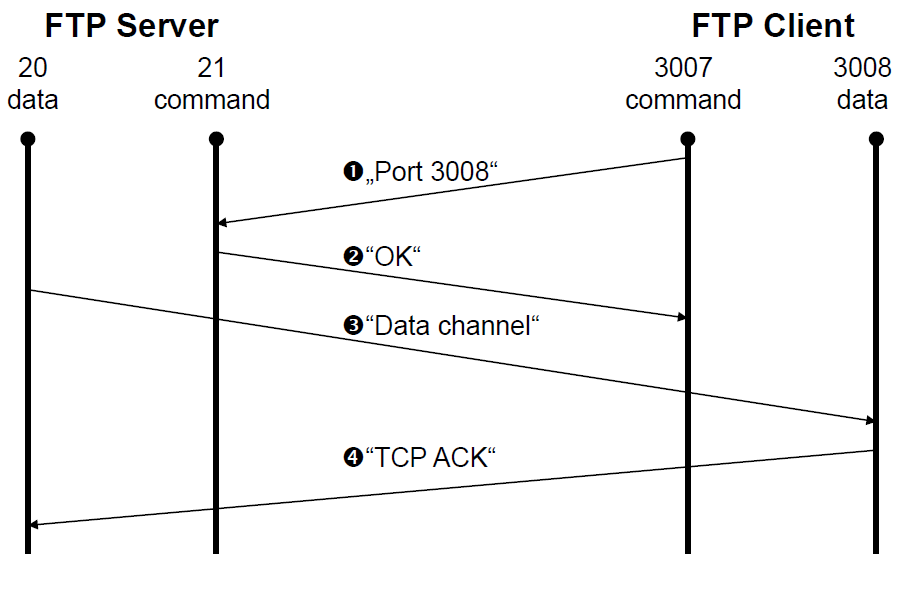
\includegraphics[width=7cm]{img/ftp_active}
	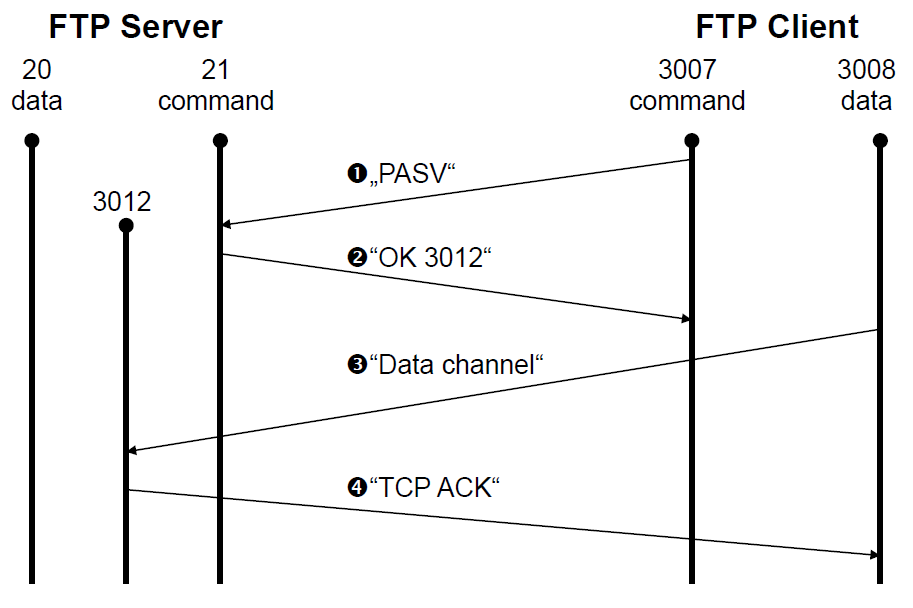
\includegraphics[width=7cm]{img/ftp_passive}	
\end{center}	


\section{Peer-to-Peer}
Der Tausch von Dateien und Streams jeder Art wurde zur Anwendungen des Internets, die die meiste Bandbreite verbraucht (geschätzt bis 75 Prozent). Bekannte P2P-Beispiele sind: \\
eDonkey, eMule, Gnutella, LimeWire, Napster (bis 2001), Bit-Torrent, FastTrack\\


P2P Netze stellen eine Alternative zu zentralisieren Strukturen dar und bringen eine Reihe von Herausforderungen mit sich:
	\begin{itemize}
	\item Finden der gesuchten Information
	\item Geschickte Verteilung der Downloads
	\item Kein Verlass auf Peers und Verbindungen
	\item Wie kann die Funktionstüchtigkeit eines P2P Netzwerkes sichergestellt werden?
	\end{itemize}
\subsection{Rechtliche Aspekte}
	\begin{itemize}
	\item Überwiegende Resistenz gegen staatliche Eingriffe.
	\item Störungssicherheit durch chaotische Organisation. 
	\item Zensur von Informationen ist nahezu unmöglich. 
	\item Legislative \glqq Störungen\grqq – Beschränkung der Macht von Gesetzgebern – Echte P2P Systeme sind von keiner Regierung zu kontrollieren. 
	\item Urheberrechte wurden in den meisten Ländern verschärft.
	\item Einführung neuer Straftatbestände.
	\end{itemize}
\subsection{Organisation der Daten}
Einige P2P Netzwerke benutzen \textbf{zentrale Server} (Tracker), an denen sich alle beteiligten Peers anmelden. Andere implementieren \textbf{verteilte Suchstrategien}, um ohne zentralen Server auszukommen. 

\subsection{Suchstrategien}
\textbf{\glqq Alle\grqq fragen (Broadcast)}
	\begin{itemize}
	\item Funktioniert nur in kleinen Domains 
	\item Zahl der Anfragen steigt mit der Zahl der Peers 
	\item Je mehr Peers vorhanden sind, desto ungünstiger wird das Verhältnis zwischen Anfragebearbeitung und \glqq eigentlicher\grqq Diensttätigkeit 
	\end{itemize}
\textbf{Super Peers}
	\begin{itemize}
	\item Einige Peers haben eine Sonderrolle 
	\item Normale Peers melden sich bei Super Peers an 
	\item Super Peers kennen weitere Super Peers 
	\item Anfragen werden an Super Peers gestellt und von diesen verteilt 
	\end{itemize}
\textbf{Flooding oder Web Crawling}
	\begin{itemize}
	\item Jeder Peer fragt ihm bekannte Peers. 
	\item Diese leiten die Frage im Nichterfolgsfall weiter. 
	\item \glqq Verebben\grqq der \glqq Frageflut\grqq nach einer vorgegebenen Anzahl von Peers (TTL). 
	\item Vermeidung von Kreisen durch Informationen, wer schon gefragt wurde. 
	\item \textbf{Flooding bekannt aus Verteilte Algorithmen!}
	\item Im Erfolgsfall wird mit einem Antwortpaket geantwortet, dieses enthält die Netzwerkadresse des Hosts, der die Antwort bereitstellt. Die eigentliche Anfrage erfolgt anschließend über spezielle Anfrage-Pakete.	
	\end{itemize}
	
\subsection{Beschreibung von Informationen}
Die Daten, die in einem P2P-Netzwerk angeboten werden, können durch zwei Möglichkeiten beschrieben werden:
	\begin{itemize}
	\item Eindeutige Kennzeichnung von Informationen, z.B. durch Hash-Werte, IDs etc.
	\item Umfangreiche Beschreibungen der eigentlichen Informationen mit Meta-Informationen. 
	\end{itemize}
\subsection{Eigenschaften von P2P}
\textbf{Verfügbarkeit} wird gewährleistet durch:
	\begin{itemize}
	\item Exzessive Replikation.
	\item Redundanz der Dienste. 
	\item Redundanz der Kommunikationspfade.
	\end{itemize}
\textbf{Performance} in Hinblick auf 
	\begin{itemize}
	\item Den Aufwand eine gestellte Frage zu beantworten
	\item Den Overhead für die Kommunikation und zur Steuerung
	\item[$\rightarrow$] Dezentral organisierte P2P-Netzwerke eignen sich nicht für Aufgaben, die in einer vorgegebenen Zeit erfüllt sein sollen
	\end{itemize}
\textbf{Anonymität}
	\begin{itemize}
	\item Vollständige Anonymität lässt sich mit P2P Technologie relativ einfach erreichen. 
	\item Dabei bleiben sowohl Dienste-Anbieter als auch Dienste-Client anonym. 
	\item Tunneln aller Nachrichten über verschiedene Peers. 
	\end{itemize}
	
\subsection{Beispiel BitTorrent Protocol}
P2P Protokolle stellen besondere Anforderungen an die zugrundeliegenden Algorithmen, damit die Verteilung der Daten vorteilhaft für alle geschieht. 

Das BitTorrent Protocol wurde von BitTorrent, Inc. spezifiziert. Eine Distribution besteht aus:
	\begin{itemize}
	\item Web Server – Download der Torrent-Files 
	\item Metainfo – Torrent-File 
	\item Tracker – Verwaltet die aktuell angemeldeten Clients 
	\item Client – Verteilt Teile der Nutzdatei 
	\end{itemize}
	
\subsubsection{Aufbau}	
Die einzelnen Torrent-Files sind wie folgt aufgebaut:
	\begin{itemize}
	\item Strings, denen die Länge vorgestellt wird\\
	\textit{announce44:http://tpb.tracker.thepiratebay.org/announce}
	\item Enthält alle Tracker
	\item Enthält alle \glqq Pieces\grqq
		\begin{itemize}
		\item piece$\_$length legt Länge der Teile fest, typisch sind 256KB
		\item Jedes \glqq Piece\grqq wird durch 20 Zeichen SHA-1repräsentiert. 
		\end{itemize}
	\end{itemize}
	
\subsubsection{Nachrichtenaustausch}
Nachrichten zwischen Tracker und Client werden über HTTP GET ausgetauscht:
	\begin{description}
	\item[info$\_$hash] - SHA-1 Hash aus dem Metainfo-File wird an Tracker geschickt
	\item[peer$\_$id] – 20 Zeichen lange zufällige ID, vom Client erzeugt
	\item[ip] – IP-Adresse oder Name des Clients
	\item[port] – Port, auf dem der Client arbeitet 
	\item[uploaded] – Anzahl der hochgeladenen Bytes
	\item[downloaded] -  Anzahl der heruntergeladenen Bytes
	\item[left] – Anzahl der Bytes, die Peer noch runterladen muss
	\item[event] – Optional, wird zum Beispiel zu Beginn und zum Ende gesendet.
	\end{description}
	
\subsubsection{Datenaustausch}
Der eigentliche Datenaustausch erfolgt dann P2P:
	\begin{description}
	\item[Request]  – Piece anfordern
	\item[Cancel] – Abbruch der Anforderung
	\item[Choke] – Drosseln des entsprechenden Clients
	\item[Unchocke] -  Freigabe des Clients (anderer Peer entscheidet, wer download starten darf)
	\item[Have]  – Gibt an, dass das entsprechende Piece vorhanden ist. 
	\item[Interested] – Client zeigt Interesse an. 
	\item[Piece] – enthält das gewünschte \glqq Piece\grqq 
	\end{description}
% 240, 250

\section{E-Mail}
Protokolle zum E-Mail-Versand sind POP3, IMAP und SMTP. Diese bauen auf Transport Transportprotokollen auf, wie 
	\begin{itemize}
	\item TCP auf Port 25 mit 7 bit ASCII
	\item NCP (Netwok Control Program) auf Port 25. \glqq Gibt es überhaupt noch ein laufendes NCP? \grqq
	\item X.25 könnte direkt benutzt werden, vorgeschlagen wird aber TCP over X.25
	\end{itemize}
\subsection{POP3}
Das POP3 (Post Office Protocol - Version 3)\cite{rfc1939} dient zum Abrufen eingehender Mails  und wird typischerweise eingesetzt, wenn direkter Mail-Empfang nicht möglich ist. Dies kann dann eintreten, wenn bspw. keine permanente Verbindung besteht, zu wenig Ressourcen beim Client bzw. Host zur Verfügung stehen oder auch wenn \glqq postlagernde\grqq Mails aberufen werden.\\
Obwohl POP3 eigentlich unabhängig vom Transport Protkoll ist, ist es nur für TCP auf Port 110 spezifiziert.
\subsubsection{Arbeitsweise}
\textbf{Kommandos} bestehen aus einem Schlüsselwort und eventuell aus Argumenten. \textbf{Antworten} bestehen aus Status, Schlüsselwort und eventuell nachfolgenden Informationen 
\subsection{Zustände und Kommandos des Servers}
	\begin{description}
	\item[AUTHORIZATION] - Phase der Authentisierung 
		\begin{description}
		\item[USER] - Übergabe des Benutzernames 
		\item[PASS] - Übergabe des Passworts (nur nach USER) 
		\item[APOP](Optional) - Übergabe es MD5 Hashes anstatt eines Passworts
		\item[QUIT] - Schließen der Verbindung 
		\end{description}
	\item[TRANSACTION] - Phase der Datenübertragung 
			\begin{description}
			\item[LIST]\textbf{$[$msg$]$} - Listet die vorhandenen Nachrichten auf. Zum einfacheren Parsen der Resultate ist das Ergebnis-Format streng vorgeschrieben
			\item[RETR]\textbf{msg} - Abholen der Nachricht mit der Nummer msg, wobei das Nachrichtenende mit . <CR><LF> gekennzeichet ist.
			\item[TOP]\textbf{msg n} - Mit diesem optionalen Befehl werden die ersten n Zeilen der Nachricht mit der Nummer msg abgeholt
			\item[DELE]\textbf{msg} - Löschen der Nachricht mit der Nummer msg 
			\item[RSET] - Reset des Servers, alle zum Löschen markierten Nachrichten werden demarkiert 
			\item[STAT] - Liefert die Anzahl der Mails und die Gesamtgröße zurück 
			\item[UIDL]\textbf{$[$msg$]$} - Gibt für jede bzw. die Nachricht mit der Nummer msg einen Unique Identifier aus 
			\item[NOOP] - Tue nichts - sinnvoll, um die Session am Leben zu halten 
			\item[QUIT] - Schließen der Anwendung und Übergang in UPDATE State 
			\end{description}
	\item[UPDATE] - Phase beim Beenden und alle zum Löschen markierten Mails werden gelöscht 
	\end{description}
\subsection{IMAP4}
Das IMAP4\cite{rfc1730} (Internet Message Access Protocol  - Version 4) ermöglicht, dass Nachrichten auf dem Server verbleiben und dort effektiv verwaltet werden. Das Protokoll ist nur für das Empfangen von Nachrichten zuständig, aber Nachrichten können auch in einzelnen Mailboxen erzeugt werden.
\subsubsection{Zustände des Servers}
\begin{center}
	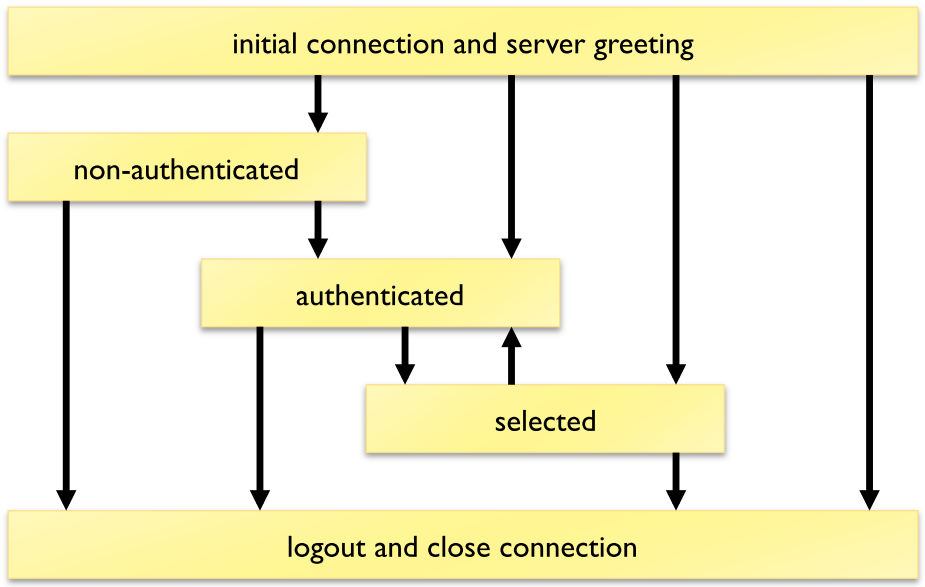
\includegraphics[width=10cm]{img/imap.png}
\end{center}
\subsubsection{AUTHENTICATE}
Die Anmeldung mittels IMAP4 kann bspw. mittels Challenge Response, wie Kerberos, erfolgen. Alternativ kann der CLient verschiedene Authentisierungsverfahren vorschlagen. Als Ausweg, wenn Authentisierung über Challenge-Response nicht funktioniert, kann ein Login genutzt werden.
\subsubsection{SELECT}
Im Zustand \textbf{selected} wurde eine Mailbox ausgewählt. Dieser Zustand wird nach einem erfolgreichen Auswählen betreten. Erreicht wird dieser Zustand mit dem Select-Befehl, der eine Mailbox auswählt. Nachfolgende Kommandos beziehen sich dann auf die selektierte Mailbox.
\subsubsection{Befehle}
	\begin{description}
	\item[EXAMINE] Als Statusanfrage zum Überprüfen einer Mailbox auf ungelesene Mails. \\
	Laut RFC: \textit{The EXAMINE command is identical to SELECT and returns the same output; however, the selected mailbox is identified as read-only.}
	\item[CREATE] - Anlegen einer Mailbox
	\item[RENAME] - Unbenennen einer Mailbox
	\item[DELETE] - Löschen einer Mailbox 
	\item[SUBSCRIBE] - Abonnieren einer Mailbox 
	\item[UNSUBSCRIBE] - Kündigen eines Abonnements
	\item[LIST path selector] - Anzeige der verfügbaren Mailboxen unterhalb des path gemäß des selectors 
	\item[SEARCH] - Suche innerhalb von Mailboxen auf dem Server
	\item[FETCH] - Liefert Nachrichten vom Server durch eine Auswahl nach Bedingungen bzw. Flags. Außerdem können Nachrichtenteile angegeben werden, die man haben möchte.
	\item[PARTIAL] - Wie FETCH, aber mit Einschränkung der Länge der zu liefernden Teile 
	\item[STORE] - Ablegen einer Nachricht in einer Mailbox, z.B. nach Änderungen 
	\item[COPY] - Kopieren einer Nachricht von einer Mailbox in eine andere
	\item[UID] - Ausgabe eines eindeutigen Identifiers für jede Nachricht
	\end{description}

\subsubsection{Mögliche Auswahlkriterien}
	\begin{itemize}
	\item Ungesehene Mails
	\item Nach Datum
	\item Nach Absender
	\item Nach TAG (\glqq Wichtig\grqq,\glqq Unwichtig\grqq etc.)
	\end{itemize}

\subsection{SMTP}

Das SMTP (Simple Mail Transfer Protocol)\cite{rfc821} ist von der zugrundeliegenden Übertragungsart unabhängig. Es benötigt lediglich einen zuverlässigen, geordneten Datenstream. Zwischen den Kommunikationspartnern (Sender-SMTP und Receiver-SMTP) wird ein Zwei-Wege-Kommunikation-Kanal aufgebaut. Dabei kann der Receiver-SMTP entweder das Ziel oder ein Zwischenglied sein. Vom Sender werden Commands an den Receiver gesendet, dieser antwortet mit Replies. 
\begin{center}
	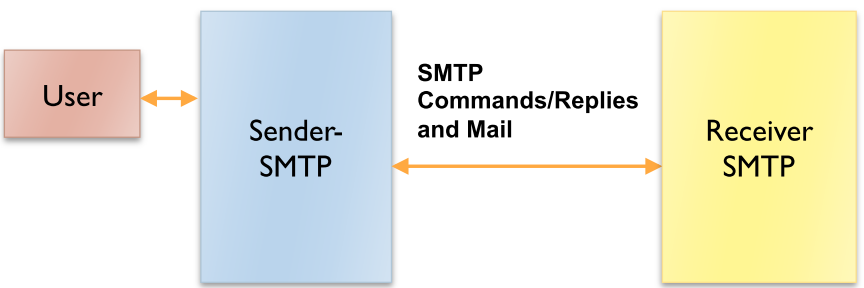
\includegraphics[width=10cm]{img/smtp.png}
\end{center}
\subsubsection{Arbeitsweise}
	\begin{itemize}
	\item Once the transmission channel is established, the SMTP-sender sends a \textbf{MAIL} command indicating the sender of the mail. 
	\item If the SMTP-receiver can accept mail it responds with an \textbf{OK} reply.
	\item The SMTP-sender then sends a \textbf{RCPT} command identifying a recipient of the mail. 
	\item If the SMTP-receiver can accept mail for that recipient it responds with an \textbf{OK reply}; if not, it responds with a \textbf{reply rejecting} that recipient (but not the whole mail transaction). 
	\item The SMTP-sender and SMTP-receiver may negotiate several recipients. When the recipients have been negotiated the SMTP-sender sends the mail data, terminating with a special sequence.  
	\item SMTP Commands:
	\end{itemize}
	\begin{verbatim}
S: MAIL <SP> FROM:<reverse-path> <CRLF> 
S: RCPT <SP> TO:<forward-path> <CRLF> 
S: DATA <CRLF> 
	\end{verbatim}

\subsubsection{Beispiel}	
	\begin{verbatim}
S: RCPT TO:<Green@Beta.ARPA> 
R: 550 No such user here 

S: RCPT TO:<Brown@Beta.ARPA> 
R: 250 OK 

S: DATA 
R: 354 Start mail input; end with <CRLF>.<CRLF> 

S: Blah blah blah... 
S: <CRLF>.<CRLF> 
R: 250 OK 
	\end{verbatim}

\subsubsection{Weiterleitung}
Wenn ein Sender eine Daten an einen Receiver sendet, um sie daraufhin an einen Empfänger weiterzusenden, gibt es zwei Reaktionsmöglichkeiten zum Forwareding:
	\begin{enumerate}
	\item  Receiver kennt den Pfad zum Empfänger und übernimmt die Verantwortung für die Zustellung
		\begin{verbatim}
		R: 251 User not local; will forward to <forward-path>
		\end{verbatim}
	\item  Receiver kennt den Pfad, aber will Mail nicht selbst zustellen
		\begin{verbatim}
		R: 551 User not local; please try <forward-path>
		\end{verbatim}
	\end{enumerate}
Was passiert, wenn sich nach Annahme der Mail durch einen Relayer herausstellt, dass Empfänger doch nicht erreichbar ist? Beispielsweise so wie in Möglichkeit 1.
	\begin{itemize}
	\item Receiver muss eine Fehlermeldung generieren. 
	\item Wohin wird diese Fehlermeldung gesendet? 
	\item Was passiert bei mehrstufigem Forwarding? 
	\end{itemize}
Um dies zu Lösen wird beim Forwarding jeweils der Pfad mitaufgenommen. Die Fehlermeldung gelangt auf dem umgekehrten Pfad zurück zum Empfänger. Typischerweise existiert für eine Gruppe von Usern ein Relay Host, der Mails für beliebige Empfänger entgegennimmt und weiterleitet.\\
Es wird zwischen Zwei Konzepten unterschieden:
	\begin{itemize}
	\item Adresse (Wer ist der Empfänger?) 
	\item Route (Wie gelangt man zum Empfänger?) 
	\end{itemize}
Des Weiteren gibt es eine Reihe von Befehlen:
	\begin{itemize}
	\item \textbf{VRFY} - Fordert den Server auf eine Adresse zu überprüfen
	\item \textbf{EXPN} - Dieser Befehl fragt nach einer Namensauflösung. Es werden je nach Berechtigung die Mitglieder einer Mailingliste ausgegeben.
	\item Nachricht am Terminal des Users ausgeben
		\begin{verbatim}
		SEND <SP> FROM:<reverse-path> <CRLF>
		\end{verbatim}
	\item Nachricht am Terminal ausgeben oder in die Mailbox legen
		\begin{verbatim}
		SOML <SP> FROM:<reverse-path> <CRLF> 
		\end{verbatim}
	\item Nachricht am Terminal ausgeben und in die Mailbox legen
		\begin{verbatim}
		SAML <SP> FROM:<reverse-path> <CRLF>
		\end{verbatim}
	\item HELO, QUIT, TURN, HELP, RSET, NOOP		
	\end{itemize}
% 260

\section{Autokonfiguration}
Dieser Abschnitt soll sich mit Technologien zur automatischen Konfiguration von Geräten und Diensten beschäftigen. Die automatische Konfiguration von Geräten kann zentral von einem Server oder dezentral durch Abstimmung zwischen den Geräten erfolgen. Dabei bieten sich zwei Strategien an:
	\begin{itemize}
	\item Geräte bieten permanent ihre Dienste an (Advertisements)
	\item Dienstenutzer fragen nach dem gewünschten Dienst
	\end{itemize}
\subsection{Motivation}
 	\begin{itemize}
	\item Wachsende Anzahl vernetzter Geräte
	\item Mobilität (PDA, Notebook, Handy)
	\item Vordringen rechnergestützter Systeme in neue Einsatzbereiche (Home/Office Automation)
	\item Neue Medien und Inhalte
	\item Vereinfachung der Administration
	\end{itemize}
	
\subsection{Discovery}
	\begin{enumerate}
	\item Anfragebasiert
		\begin{itemize}
		\item Gerät oder Client fragt in den Raum nach einem Anbieter von Konfiguration oder Diensten. 
		\item Anbieter lauscht und antwortet auf Anforderung. 
		\end{itemize}
	\item Mittels Advertisements 
		\begin{itemize}
		\item Anbieter von Diensten oder Konfigurationsdaten macht von sich aus auf sich aufmerksam. 
		\item Sendet Bekanntmachungen an alle.
		\item Clients lauschen einige Zeit.
		\end{itemize}
	\item Broadcasts / Multicasts für Anfragen in den Raum.
	\end{enumerate}
Dies lässt sich \textbf{optimieren}: Broadcasts / Multicasts zum Finden des Konfigurationsservers sind nur einmal notwendig. Danach ist wiederholtes Anfragen beim gefundenen Server möglich. \\
Ebenso ist eine Konfiguration ohne zentralen Server möglich. Dabei kann es jedoch zu Kollisionen kommen, die erkannt werden müssen.\\

Eine Alternative stellen \textbf{Registries} da: Dienste können bei einem Verzeichnisdienst registriert werden, den der Client bei der Konfiguration sucht. Der Client muss darauf hin nur einmal den gefundenen Verzeichnisdienst nach Diensten fragen.

\subsection{Leases}
	\begin{itemize}
	\item Fehler können Abbruch der Kommunikation bewirken. 
	\item Vergebene Ressourcen würden dann nicht wieder freigegeben, weshalb sie nur auf Zeit vergeben werden.
	\item Vor Ablauf der Zeit (Lease Time) muss Ressourcen-Reservierung verlängert werden. 
	\item Nach Ablauf der Lease Time wird Ressource wieder freigegeben. Client muss wissen, dass er die Ressource dann nicht mehr nutzen darf.  
	\end{itemize}
	
	
\subsection{Geräte-Integration}	
	\begin{itemize}
	\item Herstellung der Kommunikation 
	\item Einstellen von Geräte- und Netzwerkparameter 
	\item Sicherheit 
	\item Protokolle: RARP, BOOTP, DHCP, IP-Autoconfiguration, IPv6 
	\end{itemize}
\subsubsection{RARP}


\subsubsection{BOOTP}
Ursprünglich war BootP (Bootstrap Protocol) \cite{rfc951} für Diskless Workstations gedacht. Es liefert IP-Adresse und weitere Informationen, wie bspw. die Adresse eines TFTP-Servers. Die Kommunikation erfolgt via UDP.

Ein BootP-Protokoll-Paket enthält die IP-Adress-Informationen von BootP-Client, -Server und Router, sowie die vom BootP-Server vorgeschlagene IP-Adresse für den Client. Darüber hinaus hat das BootP-Frame Datenfelder für den Client-Hardwareadresse, den Server-Host-Namen, den Boot-File-Namen und ein herstellerspezifisches Feld.  


\subsubsection{DHCP}
	Das DHCP (Dynamic Host Configuration Protocol) \cite{rfc2131,rfc2132} wird zur  Übertragung von Konfigurationsparametern zu Knoten in TCP/IP-Netzen verwendet. DHCP ist abwärtskompatibel zu BOOTP.\\
	
	DHCP wird zur automatische Vergabe von IP-Adressen verwendet - und damit mehr als nur eine statische Zuordnung. Es erfolgt eine temporäre (dynamische) Zuweisung der Adressen, was DHCP zu einem aufwändigerem Protokoll macht. \\
	Es gibt verschiedene Nachrichtentypen:
		\begin{itemize}
		\item Client: DHCPDISCOVER	
		\item Server: DHCPOFFER		
		\item Client: DHCPREQUEST	
		\item Client: DCHPDECLINE	
		\item Server: DHCPACK		
		\item Server: DHCPNACK		
		\item Client: DHCPRELEASE
		\item Client: DHCPINFORM
		\end{itemize}
	Außerdem lassen sich bestimmte Parameter anpassen:
		\begin{description}
		\item[Reqested Address] - Kann der Client beim DHCPDISCOVER angeben, um sich eine bestimmte Adresse zuweisen zu lassen. 
		\item[Lease Time] - Zeitraum für die Gültigkeit der Adresse. Angabe in Sekunden (32 Bit $\rightarrow$ max. 99 Jahre)
		\item[Option Overload] - Die Felder Server Hostname und Boot Filename des können für Optionen genutzt werden.
		\item[Server Identifier] - Erlaubt die Unterscheidung zwischen verschiedenen Serven.
		\item[Parameter Request List] - Aufzählung der Tags der Optionen, an denen der Client interessiert ist. 
		\item[Max Message Size] - Maximale Größe der vom Client akzeptierte DHCP-Nachricht.  Kleinster zugelassener Wert ist 576. 
		\item[Client Identifier] - Eindeutige ClientID. Wird vom Server zur Verwaltung der Leases verwendet (bspw. MAC-Adresse).
		\end{description}
	Die wichtigsten DHCP-Vorgänge sind:
		\begin{description}
		\item[Adressanforderung] - Initiale Anforderung von Parametern (z.B. während des Bootvorganges) aus einem unkonfigurierten Zustand heraus 
		\item[Lease-Erneuerung] - Verlängerung der Lease-Dauer der Adresse, Netzwerkschittstelle ist konfiguriert 		
		\item[Abfrage von Informationen] - Anforderung von zusätzlichen Parametern (außer Adresse), Netzwerkschittstelle ist konfiguriert, Nachricht hat keinen Einfluss auf den Lease-Status im DHCP-Server
		\item[Rückgabe der Adresse ] - Adresse vom wird Client nicht mehr beötigt, daher Information an den Server, dass Adresse zur Wiederverwendung freigegeben ist. 
		\end{description}
		
\subsection{Dienste-Integration}	
	\begin{itemize}
	\item Verfügbarkeit sicherstellen 
	\item Registrierung
	\item Sicherheit 
	\item Protokolle: UPnP, HAVi, SLP, JetSend, Jini 
	\end{itemize}
	
	\subsubsection{UPnP}
	UPnP (Universal Plug and Play) vereint Geräte- und \textbf{Dienstekonfiguration} auf der Basis von bewährteer Technologie als offene Service-Architektur. Es definiert netzwerkseitige Interaktion, die tatsächliche Implementierung ist herstellerspezifisch.\\
	UPnP verwendet bekannte Technologien wie IP, TCP, UDP, ARP, HTTP, DHCP und XML.\\
	Es stellt eine Sammlung von Protokollen dar:
		\begin{itemize}
		\item SSDP (Simple Service Discovery Protocol)
			\begin{itemize}
			\item Protokoll zur Lokalisierung von UPnP-Diensten
			\item Unterstützt Client Requests sowie Service Announcements 
			\end{itemize}
		\item GENA (General Event Notification Architecture)
			\begin{itemize}
			\item Beschreibt eine HTTP-Benachrichtigungs Architektur
			\item Eine HTTP-Ressource kann ein beliebiges Objekt sein, das Benachrichtigungen senden oder empfangen kann.
			\item Die Event-Registrierung muss vor ihrem Ablauf erneuert werden, wenn sie andauern soll
			\item Soll die Event-Registrierung vor Ablauf des Timeouts aufgehoben werden, muss sie explizit beendet werden
			\item Notification wird vom Notifier an den Arbiter geschickt, der Arbiter prüft, ob es Subscriber für den Notification Type mit 
			passendem Scope gibt, wenn ja, passt der Arbiter den SID-Header für den Subscriber an und leitet die Notification weiter. 
			\end{itemize}
		\item SOAP (Simple Object Access Protocol)
		\end{itemize}
	\subsubsection{automatische Konfiguration in UPnP}
		\begin{description}
		\item[Addressing] - Konfiguration der Netzwerk-Interfaces über DHCP oder IP-Autokonfiguration
		\item[Discovery] - Lokalisierung von Services durch Control Points oder Service Advertisement 
		\item[Description] - Akquisition der Service-Beschreibung durch den Control Point 
		\item[Control] - Benutzung des Dienstes (Interaktion Control Point-Service)
		\item[Eventing] - Asynchrone Benachrichtigung von Control Points über Zustansänderungen im Service 
		\item[Presentation] - Darstellung Services-UIs im Browser (Statuspräsentation oder Service-Steuerung)
		\end{description}
	\subsubsection{HTTPU und HTTPMU}	
	 HTTP wird von TCP als Transportschicht spezifiziert. HTTPU und HTTPMU sind Variationen von HTTP via Uni-/Multicast mittels UDP. Diese werden von SSDP und GENA verwendet, bilden aber keinen Ersatz für HTTP über TCP.
	
	
% 270, 280

\section{Dateien und Drucken}
\subsection{Herausforderungen}
\textbf{Files}\\
Das Ziel ist ein Zugriff auf Verzeichnisstrukturen über ein Netzwerk, als wären sie lokal. Wünschenswert hierbei sind: Transaktionskontrolle auf verteilte Ressourcen, Fehlermeldungen, Rechtekontrolle, Sicherheit. \\
Daten kennzeichnen sich durch den Inhalt der Files und ihre Metadaten (Name, Größe, Datumsangaben, Eigentümer, Rechte, Flags, etc.)\\


\noindent\textbf{Drucken}\\
Hier ist das Ziel das Ansprechen unterschiedlicher Drucker mit unterschiedlichen 
Druckerprotokollen und im Fehlerfall das Erhalten von Fehlermeldungen.\\

\subsection{Konzepte für Filesysteme}
\noindent\textbf{Transparenz}\\
Es sollen sowohl die Anzahl der Server und dort vorhandener Geräte als auch die Verteilung der Dateien auf unterschiedlichen Servern unsichtbar bleiben. Das Client-Programme benötigen keine Kenntnis darüber, ob ein Filesystem lokal oder remote ist. Die Geschwindigkeit des Datenzugriffs ermöglicht die Illusion eines lokalen Filesystems. \\


\noindent\textbf{Flash File Systeme}\\
Eine gleichmäßige Abnutzung durch Verteilung erreichen.\\

\noindent\textbf{Transaktionale Filesysteme }\\

\noindent\textbf{Schnittstelle zum Betriebssystem}\\

\noindent\textbf{Temporäre Filesysteme }\\
Häufig im RAM realisiert: Schneller, gemeinsamer Zugriff über übliche Dateisystem-Schnittstelle 

\noindent\textbf{Schreibbare Filesysteme für eigentlich nicht schreibbare Medien (Union Mount)}\\
Bspw. CD-ROM / DVD-ROM mit dynamisch eingeblendetem schreibbarem Bereich. \\

\noindent\textbf{RAID}\\

\noindent\textbf{Komprimierte Filesysteme}\\

\noindent\textbf{Filesysteme mit unterschiedlich schnellen Medien}\\

\subsection{empty}
\noindent\textbf{Qualitätsfaktoren}\\
Das Ziel ist ein gering halten der Latenz beim Bedienen von Anfragen:
	\begin{itemize}
	\item Lokale Systeme: Laufwerkszugriffe und Verarbeitungsgeschwindigkeit (CPU)
	\item Zusätzlich bei remote Zugriff: Netzwerklatenz für Anfrage, Netzwerklatenz für Ergebnis, Bandbreite
	\end{itemize}
	
	

\noindent\textbf{Nebenläufigkeit}\\
Nebenläufigkeit ist bereits bei Mehrbenutzermaschinen lokal notwendig, also eigentlich kein spezifisches Problem von Netzwerk-Dateisystemen. Es besitzt nur eine etwas höhere Komplexität durch zwischengeschaltetes Netzwerkprotokoll. \\
Des Weiteren ist eine unterschiedliche Granularität von Locks notwendig (File-Systeme, Files, Blocks)\\



\noindent\textbf{Zugriffssteuerung}\\
Transparente Umsetzung der lokalen Mechanismen, wie Zugriffsmatrix und ACL.

\subsection{Probleme}
	\begin{itemize}
	\item Zeichenkodierung 
	\item Netzwerkprobleme während offener Transaktionen 
	\item Timeouts notwendig, um mit Netzwerkproblemen umzugehen 
	\item Replikation und Fehlertoleranz. 
	\item Historisierung. 
	\item Archivierung. 
	\end{itemize}

\subsection{Protokolle}
\subsection{NFS}
Das NFS (Network File System) \cite{rfc3530} ist in Version 4 und unterstützt UDP, TCP und Dateien, die größer als 4GB sind. Eine Authentisierung über IP-Adresse wird unterstützt.\\
	\begin{itemize}
	\item \textbf{zustandsbehaftetes Protokoll}
	\item Kryptografisch abgesichert
	\item Verteiltes Filesystem, bei dem Zugriffe nicht die Übertragung der gesamten Datei erfordern.
	\item NFSv4 bietet \textbf{Authentisierung} von Server und Client über 
	Kerberos 5 – der eigentliche Benutzer wird nicht 
	authentisiert. 
	\end{itemize}
\textbf{Arbeitsweise}
	\begin{itemize}
	\item Client meldet sich beim Server an
	\item Client erhält Client-ID als Lease
	\item Client kann File Handles anfordern (persistent oder volatile - flüchtig)\\
	\textit{Für volatile Handles ist nicht garantiert, dass sie gültig und 	persistent für die Dauer der Lebenszeit des Dateisystems auf das Dateisystemobjekt (File, Directory) verweisen. Server kann zu einer beliebigen Zeit entscheiden, dass ein volatile FH ungültig wird. }
	\item Client führt Dateioperationen auf dem Handle au
	\end{itemize}
NFS kann optimiert werden in dem mehreren Requests und Responses zusammengefasst werden. (Beispielsweise LOOKUP, OPEN, READ) Operationen können mit AND oder OR verknüpft werden und die Auswertung erfolgt in vorgegebener Reihenfolge.\\

\noindent Es gibt Procedures (\textit{NULL, COMPOUND})und eine Vielzahl von Operationen (\textit{ACCESS CLOSE, COMMIT, CREATE, GETATTR, LINK, LOCK, LOOKUP, OPEN, PUTFH, REMOVE, READ, READDIR, SAVEFH, SECINFO, WRITE,...})\\

\noindent\textbf{Retransmission}: Server darf Requests über zuverlässige Protokolle (TCP) nicht ignorieren. 

\noindent\textbf{Filehandles}: Server wandelt Filehandles in Repräsentation des lokalen Filesystems um. Nahezu alle RPC Calls benötigen ein Filehandle. Daher erfragt der Client zuerst das Root-Filehandle. Der Server liefert Attribute des FH.\\

\noindent\textbf{File Attributes}: es gibt 3 Gruppen
	\begin{itemize}
	\item Mandatory Attributes müssen von jedem Client und Server unterstützt werden.\\
	Bspw. filetype, change, leaseTimem...
	\item Recommended Attributes: Client kann jederzeit danach fragen, muss aber damit rechnen, keine Antwort zu erhalten. Server müssen Anfragen korrekt oder nicht beantworten.
	\item Named Attributes sind nicht im NFS Protokoll vorgesehen, können aber über Strings angefragt werden. 
	\end{itemize}

\noindent Beim Server \textbf{Pseudo Filesystem}  ersetzt der Server  fehlende Teile im Namespace, die nicht exportiert werden, durch Pseudo FS.\\

\noindent Für das \textbf{Locking} identifiziert sich der Client mit einer Client ID. Wenn Client abstürzt, wird neue Inkarnation des Clients SETCLIENTID aufrufen. Dadurch werden alle alten Leases der alten Inkarnation auf dem Server ungültig.\\

\noindent\textbf{OPEN} ist immer vorgeschrieben, auch wenn keine Operationen oder exklusiver Zugriff gewünscht sind. Vor \textbf{CLOSE} sollen alle Locks freigegeben werden.
 
\subsection{SMB / CIFS}
Ursprünglich wurde SMB (Server Message Block) für Windows und OS/2 entwickelt. Es ist aber kein Standard-Dokument verfügbar, da einige Features geheimgehalten werden sollen. (Reverse Engineered für Samba Entwicklung)\\
Umbenennung 1996 von SMB in Common Internet File System (CIFS), neue Features. 
CIFS baut dabei auf NetBIOS over TCP/IP und SMB auf und bietet neben der Datei- und Druckerfreigabe weitere Dienste wie zum Beispiel den Windows-RPC- und den NT-Domänendienst an. 
\subsection{WebDAV}
	\begin{itemize}
	\item HTTP Extensions for Web Distributed Authoring and Versioning \cite{rfc4918}
	\item Erweiterung von HTTP durch neue Requests. \\
	(\textbf{COPY, MOVE, LOCK / UNLOCK, DELETE, MKCOL, PROPFIND / PROPPATCH})
	\item Properties als XML Dokument 
	\item Datei muss vollständig übertragen werden, dann geändert, dann zurück übertragen. 
	\end{itemize}
\subsection{iSCSI}
Das ISSCSI (Internet Small Computer Systems Interface)\cite{rfc3720} benutzt TCP als Transport für SCSI Kommandos (quasi Tunneln)  typischerweise Port 860 und 3260.Das SCSI-Gerät verhält sich für das Client-System Initiator) wie ein lokales Gerät.
	\begin{itemize}
	\item Der Initiator (Client) kann entweder aus Software oder Hardware erstellt werden. 
	\item Target (Server) kann ebenfalls als Software oder Hardware realisiert werden. 
	\end{itemize}
Die iSCSI Adressierung erfolgt durch:
	\begin{itemize}
	\item Hostname oder IP Adresse 
	\item Port 
	\item iSCSI Name
	\end{itemize}

% 300, 310

\section{Telnet, SSH und rlogin}
%PRÜFEN Qualitätskontrolle für den gesamten Abschnitt nötig, Folien geben nicht viel her!
% 320
\subsection{Telnet}
Telnet wird genutzt, um eine allgemeine, bidirektionale, 8-bit-orientierte Kommunikation zu ermöglichen und so mit entfernten Terminalen und terminal-orientierten Prozessen zu kommunizieren.
Es verwendet den TCP-Port 23, wobei es ursprünglich NCP genutzt hat.
Auf beiden Enden der Verbindungen werden Network Virtual Terminals (NVT) angelegt.
Diese handeln \emph{Options} aus (z.B. Character Set, Binary Transmission, Echo,Status, Timing Mark Option usw.)

\textbf{Jedoch: } Keine Verschlüsselung der Daten. Keine Authentisierung
auf Paket-Ebene. Tunnel durch TLS natürlich möglich.

Einzige sinnvolle Anwendung für Telnet heutzutage ist \texttt{telnet towel.blinkenlights.nl} und die Vorort-Konfiguration von Geräten (z.B. Switches oder Router).
\subsection{Secure Shell}
SSH\cite{rfc4251} ermöglicht eine kryptografisch abgesicherte Terminal-Verbindung.
Es nutzt RSA und DSH\footnote{Distributed Shell, warum steht das hier?}
Außerdem wird eine Authentisierung über Public Key ermöglicht.
SSH-Server lauschen für gewöhnlich auf TCP-Port 22.
\subsection{rlogin}
rlogin\cite{rfc1258} lauscht auf TCP-Port 513.
Nach Verbindungsaufbau sendet der Client vier Strings:
\begin{itemize}
	\item \textless null \textgreater
	\item client-user-name\textless null\textgreater
	\item server-user-name \textless null\textgreater
	\item terminal-type/speed \textless null\textgreater
\end{itemize}
Server antwortet mit Null-Byte.
Flusskontrolle über START- und STOP-Zeichen.
Dimensionen des Ausgabefensters werden übertragen.
Sicherheit wie telnet, hinzu kommt, dass viele Implementierungen Passwort-Eingabe für einzelne Clients (nach IP-Adresse) abschalten können.
\section{Extensible Messaging and Presence Protocol (XMPP)}
XMPP ist aus dem Jabber-Protokoll hervorgegangen und wird von diesem als Grundlage genutzt. Google Talk nutzt es ebenfalls.\\
	\begin{itemize}
	\item Offener Standard,kostenfrei nutzbar, nicht an einen Hersteller gebunden, freie Libraries 
	\item Kommunikation Client-Server-Client, nicht direkt Client-Client. 
	\item Kein zentraler Server notwendig (jeder kann einen Server betreiben), Adressierung ähnlich wie bei E-Mail 
	\item XMPP-Server sind untereinander verbunden. 
	\item XMPP basiert auf XML als Steam (der kein vollständiges XML-Dokument enthält)
	\item TCP Port 5222 
	\item Übertragung von Binaries über andere Protokolle (http) oder notfalls als base64 (quasi Binary als ASCII) 
	\item Verbindungen zu anderen Protokollen sind möglich (Translation durch Gateways) 
	\item XMPP kann über HTTP getunnelt werden - Entweder durch regelmäßige Requests (Polling) oder durch Requests mit stark verzögerter Antwort (Binding) 
	\item Benutzung von TLS und Simple Authentication and Security Layer (SASL) ist standardisiert
	\item Fehlermeldungen werden ebenfalls als XML Standard übertragen 
	\end{itemize}
% 330

\section{LDAP}
Das Lightweight Directory Access Protocol ist ein Netzwerkprotokoll zur Abfrage und Änderung von Informationen verteilter Verzeichnisdienste.  Es beschreibt die Kommunikation zwischen dem LDAP-Client und dem Verzeichnis-(Directory-)Server. Aus einem solchen Verzeichnis können objektbezogene Daten, wie zum Beispiel Personendaten oder Rechnerkonfigurationen, ausgelesen werden. Die Kommunikation erfolgt auf Basis von Abfragen. $[Wikipedia]$
\subsection{Structure}
	\begin{itemize}
	\item Nutzt einen verbindungsorientierten zuverlässigen Transport: TCP auf Port 389
	\item Connection Oriented Transport Service (COTS) - mapped LDAP Nachrichten PDU direkt auf T-Data (???)
	\item Es wird X.500 zur Organisation von Verzeichniseinträgen in einem hierarchischen Namespace genutzt - ermöglicht Suchen.
	\item Used to access and update information in a directory built on the X.500 model 
	\item Specification defines message format between client and the server 
	\item Includes session handling (connect, disconnect etc.) 
	\end{itemize}
\noindent\textbf{Information}: Structure of information stored in an LDAP directory.\\
\noindent\textbf{Naming}: How information is organized and identified.\\
\noindent\textbf{Functional / Operations }: Describes what operations can be performed on the information stored in an LDAP directory. \\
\noindent\textbf{Security}: Describes how the information can be protected from unauthorized access.
  	\begin{center}
  		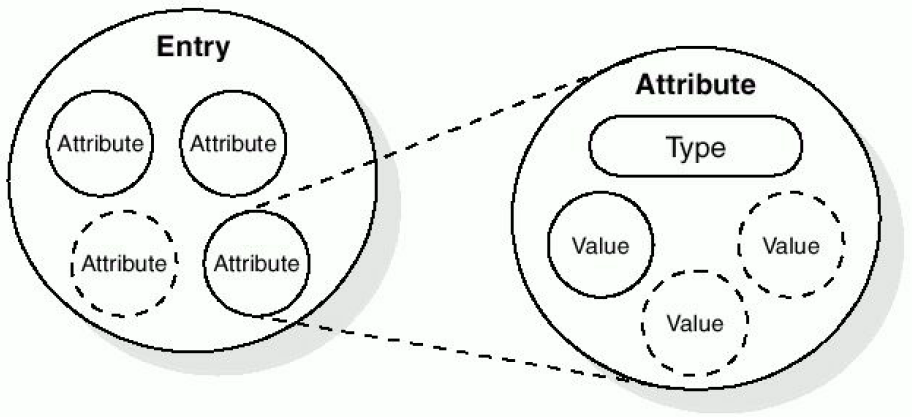
\includegraphics[width=10cm]{img/LDAPIS.png}
  	\end{center}
Bei der LDAP Informationsspeicherung beschreibt jeder Eintrag ein Objekt einer Klasse
	\begin{itemize}
	\item Beispiel Eintrag: \textit{InetOrgPerson(cn, sn, ObjectClass)}
	\item Beispiel Attribute: \textit{cn (cis), sn (cis), telephoneNumber (tel), ou (cis), owner (dn),jpegPhoto (bin) }
	\end{itemize}
(\textit{cn common name, dn distinguished name, sn surname})
\subsection{Naming}
Distinguished names consist of sequence of Relative DN \textit{cn=John Smith,ou=Austin,o=IBM,c=US (Leaf 2 Root) } \\
Ein Directory Information Tree (DIT) folgt einem graphischen oder organisiertem Schema. \\
Aliases can link non-leaf nodes.\\

\noindent\textbf{Schema:}
	\begin{itemize}
	\item Definiert welche Objekt-Klassen erlaubt sind
	\item Wo diese gespeichert sind
	\item Welche Attribute sie besitzen bzw. optional sind
	\item Von welchem Typ/welche Syntax jedes Attribut besitzt
	\item Das Schema muss für den Client lesbar sein
	\end{itemize}

\subsection{Functions/Operations}
Zur Verteilung von strukturierten Informationen in einem Netzwerk (Authentifikation, Registry Informationen)	
	\begin{itemize}
	\item Authentifikation(BIND/UNBIND, ABANDON)
		\begin{itemize}
		\item BIND-Request includes LDAP version, the name the client wants to bind as, authentication type
		\item Server responds with a status indication 
		\item UNBIND: Terminates a protocol session
		\item ABANDON:  MessageID to abandon
		\end{itemize}
	\item Query (Suche, Einträge vergleichen)
		\begin{itemize}
		\item Request includes baseObject, Scope, derefAliases, sizeLimit, timeLimit, attrsOnly, Filter, Attributes
		\item Read and List implemented as searches 
		\item Compare: similar to search but returns T/F
		\end{itemize}
	\item Update (Einträge hinzufügen/löschen, modifizieren)
	\item Other Requests: Search/modify/delete/change requests can include maximum time limits (and size limits in the case of search). There can be multiple pending requests.
	\end{itemize}	

\subsection{Client and Server Interaction}
	\begin{itemize}
	\item Client establishes session with server (BIND)
		\begin{itemize}
		\item Hostname/IP and port number 
		\item Security(authentication, Encryption/Kerberos supported)
		\end{itemize}
	\item Client performs operations ()Read/Update/Search)
	\item Client ends the session (UNBIND) 
	\item Client can ABANDON the session 
	\end{itemize}



\subsection{Security}
	\begin{itemize}
	\item Clear text passwords (version 1)
	\item KERBEROS version 4 authentication
	\item SSL
	\end{itemize}

\subsection{Protocol Model}
Clients performing protocol operations against servers.
	\begin{itemize}
	\item Client sends protocol request to server 
	\item Server performs operation on directory 
	\item Server returns response (results/errors)
	\end{itemize}
Asynchronous behavior 

\subsection{Search Request Parameters }
	\begin{itemize}
	\item base\\
		\textit{The base is the DN of root of the search. A server typically serves only below some subtree of the global DN namespace.}
	\item scope 
			\begin{itemize}
			\item base – search only the base element. 
			\item onelevel – search all elements that are children of the base. 
			\item subtree – search everything in the subtree base
			\end{itemize}
	\item size \\
		\textit{Limit on the number of entries to return from the search. A value of 0 means no limit.}
	\item time \\	
		\textit{Limit on number of seconds the search can take. Value of 0 means no limit.}
	\item attributes \\
		\textit{A list of attributes that should be returned for each matched entry. NULL mean all attributes. Attribute names are strings.}
	\item attrsonly \\
		\textit{a flag that indicates whether values should be returned}
	\item search$\_$filter  
			\begin{itemize}
			\item a search filter that defines the conditions that constitute a match. 
			\item Filters are text strings. 
			\item There is an entire RFC that describes the syntax of LDAP filters.\\
			(RFC 1558 oder 1960 $\rightarrow$ Widerspruch in den Folien) 
			\end{itemize}
	\end{itemize}
\subsection{Search Filters}
	\begin{itemize}
	\item Restrict the search to those records that have specific attributes, or those whose attributes have restricted values. 
	\item You can combine simple filters with boolean $\&$,| and !
	\end{itemize}
Beispiele:
	\begin{itemize}
	\item objectclass=* \textit{ match all records }
	\item cn=*dave* \textit{ matches any record with dave in the value of cn }
	\item ($\&$(cn=*da)(email=*hotmail*)) 
	\end{itemize}
\noindent\textbf{Search Reply}
	\begin{itemize}
	\item Each search can generate a sequence of Search Response records: \\
	\textit{Distinguished Name for record, list of attributes, possibly with list of values for each attributem, Result code }
	\item LDAP includes an extensive error/status reporting facility.
	\end{itemize}
\noindent\textbf{LDAP API }
	\begin{enumerate}
	\item Open connection with a server
		\begin{itemize}
		\item int ldap$\_$bind(...) ->  LDAP$\_$SUCCESS  or ldap$\_$errno
		\item There are actually a bunch of  ldap$\_$bind functions
		\item Synchronous calls all end in \textbf{s} - Asyn. without \textbf{s}
		\end{itemize}
	\item Authenticate
			\begin{itemize}
			\item 
			\end{itemize}
	\item Do some searches/modification/deletions
	\item Close the connection
	\end{enumerate}
	
% 340

\section{Authentication Protocols}
Authentifikation ist der Prozess, bei dem versucht wird die Identität von jemanden nachzuweisen. Authentifikation ist ein wichtiger Bestandteil für Login-/Zugriffs-Prozesse, Security-Protokolle oder das Web of Trust.\\


\noindent Methoden zur Authentifikation sind Kerberos, RADIUS, PAP / CHAP / EAP 

\subsection{Prinzipien}
Es gibt eine Vielzahl von Protkollen, die unverschlüsselte Passwörter verwenden: sogenannte Plain-Text-Passwörter.\\
\textit{Telnet, FTP, POP3(teilweise, auch wenn MD5 als replay-anfällige Alternative möglich ist), IMAP4 (teilweise)}

\subsubsection{Wissensbasiert} 
Es muss eine gemeinsame geheime Information dem Authentifizierenden gezeigt werden.\\ \textbf{Probleme}: ein zu schwach gewähltes Passwort (Wörterbuch-Angriff, Brute-Force), der Nutzer vergisst sein Passwort oder das Passwort wurde kompromittiert.\\
\textbf{Beispiele}: PIN, Passwort, key phrase, personal information

\subsubsection{Besitzbasiert} 
Es muss über das Netzwerk nachgewiesen werden, dass jemand den Nachweis besitzt. Es muss eine geheime Information innerhalb des Tokens sein. Diese darf jedoch nicht über das Netzwerk übertragen, sondern nachgewiesen werden. \\
\textbf{Probleme}: Der Nutzer kann das Token verlieren oder jemand anderes kopiert es sich.\\
\textbf{Beispiele}: SmartCard / SIM card, credit card, key, RFID token, phone, transponder, PC, DRM module (inside audio player, TV set etc.) 

\subsubsection{Biometrisch} 
Biometrische Eigentschaften können nicht vergessen, gestolen, belauscht oder gelernt werden. Der Umgang kann mit unter kompliziert sein. Üblicherweise ist dies die einzige Möglichkeit eine Person an ein Gerät zu binden. Alle anderen Verfahren können von jemand anderem ausgeführt werden.
 Retina, Iris, finger print, DNA, voice, signature
 
\subsubsection{Zwei-Faktor-Authentifizierung}
Erhöht die Sicherheit um ein weiteres, wenn zwei Verfahren kombiniert werden, auch bekannt als \glqq strong authentication\grqq


\subsection{Probleme}
	\begin{itemize}
	\item Wie kann man sich sicher gegenüber jemandem ausweisen, der sich selbst nicht ausgewiesen hat? \\
	Es könnte ein Man-in-the-middle Angriff sein, Replay-Attaken müssen verhindert werden, weshalb eine gegenseitige Authentifikation notwendig ist.
	\item Wie kann man sich durch Wissen oder Besitz authentifizieren, ohne das eigentliche shared secret zu übertragen.
	\end{itemize}
Es gibt standardisierten Protokollen für eine Vielzahl von Anwendungen.
\subsection{Angriffe}
\noindent\textbf{Man in the middle}\\
Es befindet sich jemand zwischen zwei Kommunikationspartnern und wirkt für alle wie das Gegenüber. Es ist ein vertrauenswürdiger Dritter von Nöten, um solche Angriffe zu verhindern.\\

\noindent\textbf{Replay}\\
Bei diesem Angriff zeichnet der Angreifer eine verschlüsselte Authentifikations-Nachricht auf. Um Zugriff zu erhalten, spielt er sie erneut ab. Es ist notwendig für jede Authentifikations-Nachricht einen einzigartigen Wert zu verwenden. Idealer Weise ist dieser nur einmal nutzbar.\\

\noindent\textbf{Denial of service}\\
Hierbei handelt es sich gewisser Maßen um einen Akt des Vandalismus. Jemand verursacht die Kommunikation zwischen Server und Client zu stören bzw. zu blockieren. Dieser Angriff ist meist schwer zu vereiteln.


\subsection{Challenge-Response}
Dieses Verfahren ermöglicht es, dass das Wissen über ein geteiltes Geheimnis bewiesen werden kann, ohne dass es versendet werden muss. Dadurch sollen Replay-Angriffe verhindert werden.
	\begin{center}
		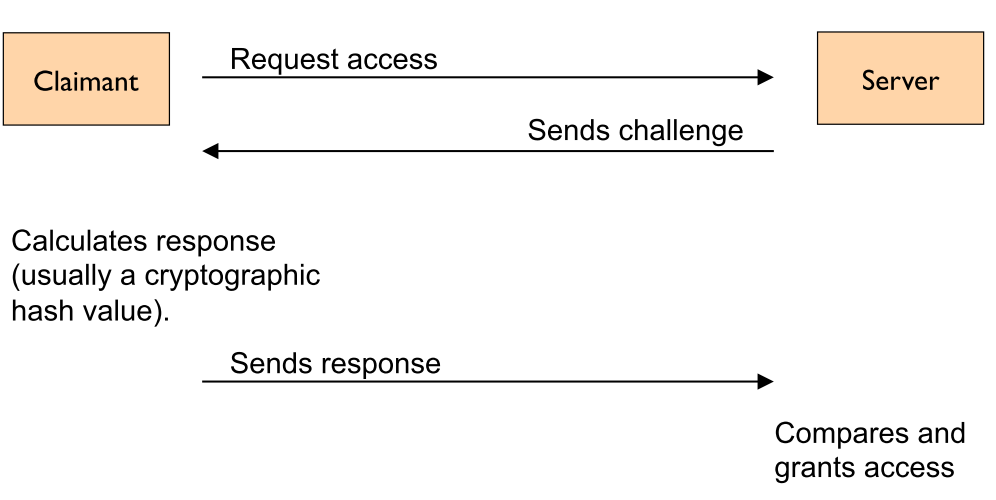
\includegraphics[width=10cm]{img/challResp.png}
	\end{center}

\subsection{Kerberos}	
%TODO RFC RFC4120 (v.5)
	\begin{itemize}
	\item Kerberos ist ein computer network authentication protocol
	\item Ermöglicht eine Kommunikation über ein unsicheres Netzwerk, bei dem die Identität des Gegenüber auf sichere Art und Weise bewiesen werden kann.
	\item Die Entwickler legten den Fokus auf das Client-Server-Model und realisierten eine \textbf{gegenseitige} Authentifikation.
	\item Kerberos ist abgesichert gegen Lauschen und replay attacks.
	\item Kerberos basiert auf dem Vergeben von Tickets. Ein solches Ticket repräsentiert ein bestimmtes Recht.
	\item Kommunikationsinstanzen:
		\begin{itemize}
		\item Client
		\item Authentication server (AS)\\
		\textit{Keeps long-term shared secrets}
		\item Ticket granting server (TGS)\\
		\textit{Issues tickets for service servers, when client presents a valid ticket from authentication server.}
		\item Service server (SS)\\
		\textit{Performs application tasks.}
		\end{itemize}
	\end{itemize}


\begin{figure}[ht]
	\centering
  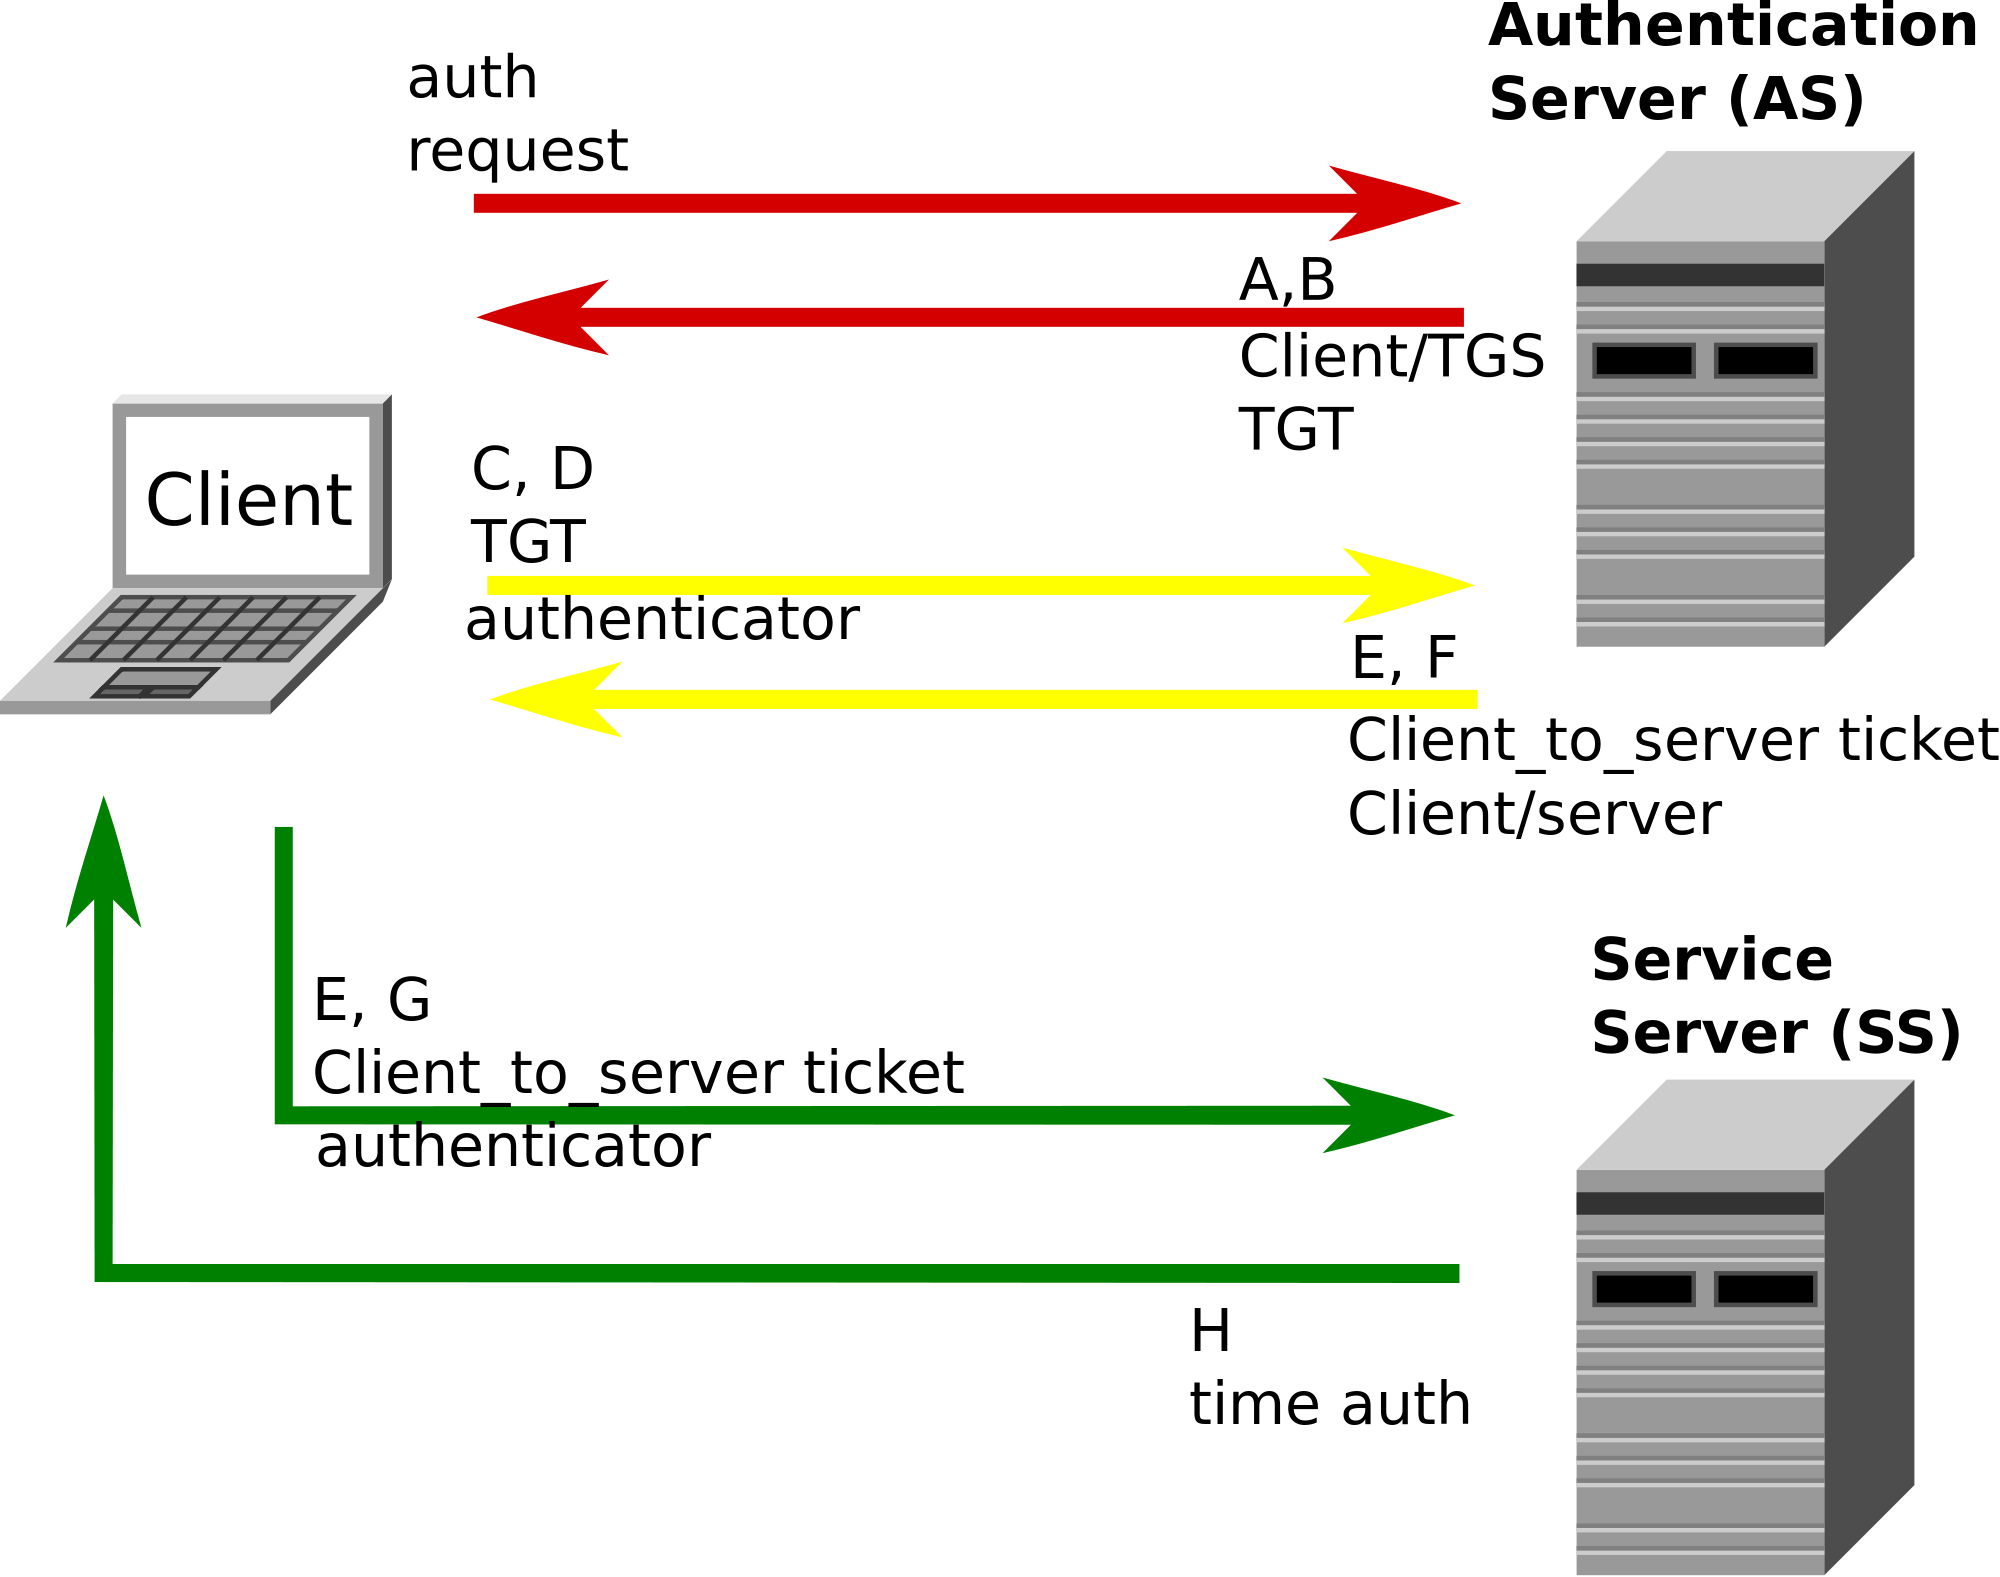
\includegraphics[width=8cm]{img/kerberos.png}
	\caption{Kerberos Ablauf (von oben nach unten) - Wikipedia}
\end{figure}
%TODO Es ist die Frage, ob hier noch mehr ins Detail gegangen werden soll - Folie 18-21

\subsection{RADIUS}
RADIUS (Remote Authentication Dial In User Service) wird wie Kerberos zur Authentifikation, Authorisation und zum Accounting von Netzwerk-Ressourcen benutzt. Es wird verwendet für DSL, wireless und VPN. Ein RADIUS Server ist außerdem in der Lage Accounting-Informationen zu sammeln - genauso wie Zugriffsaufzeichnungen und die transportierten Daten.\\

\noindent Kommunikationsinstanzen
	\begin{itemize}
	\item Client
	\item Network access server (NAS) – Server that runs an application or gateway. 
	\item RADIUS server – Server that keeps the user data base. 
	\end{itemize}
	
	\begin{enumerate}
	\item \textbf{Authentifikation}: Der Cleint erfragt Zugriff auf eine Netzwerk Ressource via NAS. Der NAS sendet den RADIUS access request zu einem RADIUS Server. Es können verschiedene Authentifikationsschemata verwendet werden (PAP, CHAP, EAP
	\item \textbf{Authorisation}: Der RADIUS Server überprüft den Client Account (bspw. via LDAP) antwortet:
		\begin{itemize}
		\item Access Accept (eventually limited for a certain time or period). 
		\item Access Reject 
		\item Access Challenge (requesting additional information). 
		\end{itemize}
	\item Accounting: Nachdem der NAS Zugriff gewährt hat, informiert er den RADIUS Server darüber \glqq accounting start\grqq. Während der Verbindung kann der NAS \glqq interim accounting records\grqq versenden. Zum Schluss wird \glqq accounting stop\grqq an den RADIUS Server gesendet. Die Nachricht kann noch Zusatzinformationen enthalten.
	\end{enumerate}
\subsection{PPP}
PPP (Point-to-Point Protocol) ist auf der Sicherungsschicht in der Internetprotokollfamilie angesiedelt. Im folgenden Sind Protokolle zuzr Authentifikation beschrieben, die für PPP eingesetzt werden.
\subsubsection{CHAP}
%TODO RFC 1994
Das Challenge Handshake Authentication Protocol (CHAP) ist ein Authentifizierungsprotokoll, das im Rahmen von PPP eingesetzt wird. 
	\begin{itemize}
	\item Ein Client initiiert eine Verbindung zu einem Einwahlserver, und dieser verlangt eine Authentifizierung mittels CHAP. 
	\item Dabei wird ein zufälliger Wert (die Challenge) an den Client übertragen, der sich authentifizieren muss.
	\item Der Client bildet aus der Zufallszahl und dem Passwort einen Hashwert mittels einer Hashfunktion (MD5, SHA-1, SHA-256) und überträgt diesen an den Einwahlserver.
	\item Der Einwahlserver errechnet ebenfalls einen Hashwert aus der Zufallszahl und dem bei ihm (im Klartext) hinterlegten Passwort. Wenn dieser mit dem vom zu authentifizierenden Rechner gesendeten Wert übereinstimmt, ist die Authentifizierung erfolgreich.
	\item In einem zufälligen Abstand sendet der Einwahlserver erneut einen zufälligen Wert (die Challenge) an den Client, und die Schritte 1–3 werden wiederholt.
	\end{itemize}

\subsubsection{PAP}
Das Password Authentication Protocol (PAP) ist ein Verfahren zur Authentifizierung über PPP und ist in RFC 1334 beschrieben. %TODO RFC verlinken
Bei PAP wird das Passwort für die Authentifizierung unverschlüsselt zusammen mit der Benutzerkennung übertragen. Der Client sendet den Nutzernamen und das Passwort. Der Server antwortet mit ack bzw. nak.

\subsubsection{EAP}
Das Extensible Authentication Protocol (EAP) ist ein  allgemeines Authentifizierungsprotokoll, das unterschiedliche Authentisierungsverfahren unterstützt wie z. B. Username/Password (RADIUS), Digitales Zertifikat, SIM-Karte. EAP wird oft für die Zugriffskontrolle in WLANs genutzt.\\
EAP spezifiziert ein Authentifikations-Framework - keinen konkreten Mechanismus. Es definiert \glqq nur\grqq das Nachrichtenformat.

\subsubsection{SSO}
Single Sign-on (SSO) bedeutet, dass ein Benutzer nach einer einmaligen Authentifizierung an einem Arbeitsplatz auf alle Rechner und Dienste, für die er lokal berechtigt (autorisiert) ist, am selben Arbeitsplatz zugreifen kann, ohne sich jedes Mal neu anmelden zu müssen. 
% 350 - 12

\section{Simple Network Management Protocol}

% 360
%PRÜFEN SNMP 

SNMP ermöglicht das Verwalten und Überwachen von Netzwerkressourcen.
Wichtige Teilnehmer sind \textbf{Agenten} und \textbf{Manager}.
Agenten sind Applikationen, die auf Netzwerkteilnehmern (Hosts, Router, Drucker etc.) laufen und Informationen über Konfiguration und Status verwalten.
Manager kontaktieren Agenten um Informationen abzufragen oder zu verändern.

Datenobjekte (z.B. \emph{Tonerstand Cyan}) werden als Object Identifier (OID) bezeichnet.
Diese sind baumartig-hierarchisch geordnet und können entsprechend auf zwei Weisen dargestellt werden:
Zum einen numerisch, etwa \texttt{1.3.6.1.2.1.4.6.} und zum anderen als Zeichenkette \texttt{iso.org.dod.internet.mgmt.mib-2.ip.ipForwDatagrams}.
Eine OID entspricht dabei einem Knoten im Baum.
\textbf{Management Information Bases} (MIB) sind Textdateien, welche diese Objekte beschreiben.
Sie werden häufig von Software eingelesen, um dem Nutzer weitere Informationen zur Verfügung zu stellen oder bekannte OIDs anzuzeigen.

Manager und Agenten kommunizieren über das SNMP.
Agenten lauschen auf UDP-Port 161.
An diesen senden Manager eine Anfrage (\texttt{get-request}) und erhalten eine Antwort (\texttt{get-respond}).
Über einen \textbf{SNMP-Walk} kann eine Reihe von aufeinanderfolgenden OIDs abgefragt werden (\texttt{get-next-request}).
Modifikationen können mit (\texttt{set-request}) vorgenommen werden.

Ebenfalls kann die Kommunikation vom Agenten initiiert werden.
Bei bestimmten Ereignissen (z.B. Tonerfüllstand $<$ 10\% oder Last auf Switch $>$ 95\%) sendet der Agent eine Nachricht an den Manager (UDP-Port 162).
Dieses Verfahren wird \textbf{SNMP-Trap} genannt.

Der \textbf{Paketaufbau} für Get/Set-Nachrichten ist relativ simpel gehalten.
Sie beginnen mit der Versionsnummer und der Community.
Die Communities stellen eine Art Passwort dar und werden im Klartext übermittelt.
Häufig akzeptieren viele Geräte \texttt{public} als Standard-Community.
SNMPv3 hat Verbesserungen der Sicherheit adressiert.

Es folgt eine \textbf{SNMP PDU}.
Wesentliche Bestandteile hierbei sind der Type (z.B. v1Get, v2Get etc), eine einmalige Request ID und eine Folge von Objekt-Wert-Paaren, die angefragt werden.
\section{Data Link Layer - MAC Sublayer}
In diesem Abschnitt werden verschiedene Konzepte zum Medienzugriff beschrieben:
\textbf{Kollisionsbehaftete Verfahren}
	\begin{itemize}
	\item Unkoordinierter (zufälliger) Zugriff auf das Medium 
	\item Kollision muss erkannt und behandelt werden		
	\end{itemize} 
\textbf{Kollisionsfreie Verfahren}
	\begin{itemize}
	\item Koordinierter Zugriff (Steuerung des Zugriffs durch dezentralisiertes oder dezentrales Verfahren) 
	\end{itemize}
	
\textbf{Zufälliger Medienzugriff}
Kann auftreten, wenn 
	\begin{itemize}
	\item ein gemeinsames Medium genutzt wird (mehr als zwei Stationen teilen sich einen Übertragungskanal). 
	\item keine zentrale Steuerung des Medienzugriffs erfolgt, keine Abstimmng mit anderen Stationen 
	\item Keine Reservierung stattfindet
\end{itemize}
Beispiele: Ethernet LAN, WLAN, Bluetooth

\subsection{Pure Aloha}
Wurde 1970 für  Funknetze an der Universität Hawaii entwickelt  um folgendes Grundproblem zu lösen: gemeinsamer Übertragungskanal (Luft), Stationen senden unkoordiniert Frames gleicher Länge aus Aussendung dauert immer eine konstante Frame-Zeit) und Kollisionen werden von allen Stationen erkannt.
\subsubsection{Ablauf}
	\begin{itemize}
	\item Wahrscheinlichkeit p wird für alle Stationen fest vorgegeben 
	\item Immer wenn genug Daten für ein Frame vorliegen, wird das Frame unverzüglich gesendet 
	\item Kollisionen sind möglich, dann wird der aktuelle Frame noch vollständig gesendet:
		\begin{enumerate}
		\item Station ermittelt ermittelt Zufallszahl k aus [0,1]
		\item Wenn k $<=$ wird Frame sofort neu gesendet, sonst wird eine Frame-Zeit gewartet (mit Wahrscheinlichkeit p wird Frame gesendet, mit Wahrscheinlichkeit (1-p) wird eine Frame-Zeit gewartet 
		\item Falls gewartet wurde, GOTO 1. 
		\end{enumerate}
	\item Die Wartezeit muss zufällig verteilt sein 
	\end{itemize}	

\begin{figure}[ht]
	\centering
  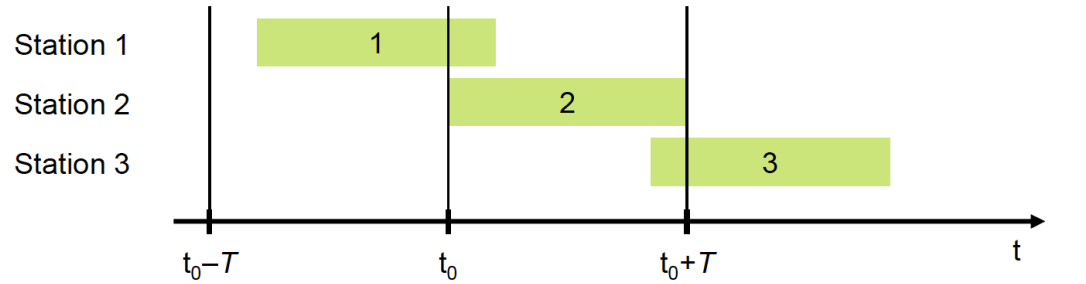
\includegraphics[width=12cm]{img/pure1.png}
	\caption{Station 2 sendet zum Zeitpunkt $t_0$  einen Frame. T ist die Frame-Zeit. Kollisionen, wenn andere Stationen im Zeitraum [$t_0–T$, $t_0+T$] mit dem Senden beginnen}
\end{figure}

\subsubsection{Erste Bewertung}
Es handelt sich um eine \textbf{einfache} Implementation. Jede Station kann die volle Kanalkapazität nutzen, solange nur sie allein Daten zu senden hat. Aber dir Auslastung des Kanals ist schlecht wegen \textbf{Retransmits} wegen Kollisionen und \textbf{Wartezeiten} nach Kollisionen.
\subsubsection{Auslastung}
Ein Frame wird genau dann erfolgreich übertragen, wenn: 
	\begin{itemize}
	\item Eine Station im Zeitraum [$t_0,t_0+T$] sendet (Wahrscheinlichkeit hierfür beträgt p) und 
	\item Keine von N–1 Stationen im Zeitraum [$t_0,t_0+T$] sendet (Wahrscheinlichkeit ist $(1–p)^{N–1}$ ) und 
	\item Keine von N–1 Stationen im Zeitraum [$t_0-T,t_0$] sendet (Wahrscheinlichkeit ist $(1–p)^{N–1}$ )
	\end{itemize}
Daraus folgt Wahrscheinlichkeit für erfolgreiche Übertragung eines Frames 
	\begin{itemize}
	\item einer ausgewählten Station: $p*(1–p)^{N–1}*(1–p)^{N–1} = p*(1–p)^{2*(N–1)}$
	\item einer beliebigen aus N Stationen: $N*p*(1–p)^{2*(N–1)}$
	\end{itemize}
Optimalen Kanalsauslastung: 0,184


\subsection{Slotted Aloha}
Änderungen gegenüber Pure Aloha
	\begin{itemize}
	\item Zeit ist in Slots eingeteilt 
	\item Die Dauer eines Slots entspricht genau der Frame-Zeit 
	\item Übertragungen beginnen immer an Anfang eines Slots 
	\item Uhren der Stationen sind synchronisiert (alle Stationen nutzen die gleiche Slot-Einteilung), z.B. durch Aussendungen des Zeitsignals auf separatem Kanal 
	\end{itemize}
Die Kollisionsbehandlung ist wie bei Pure Aloha. Der Ablauf ist anders: Sobald genügend Daten für einen Frame vorliegen, wird der Frame unverzüglich zu Beginn des nächsten Slots gesendet.
\begin{figure}[ht]
	\centering
  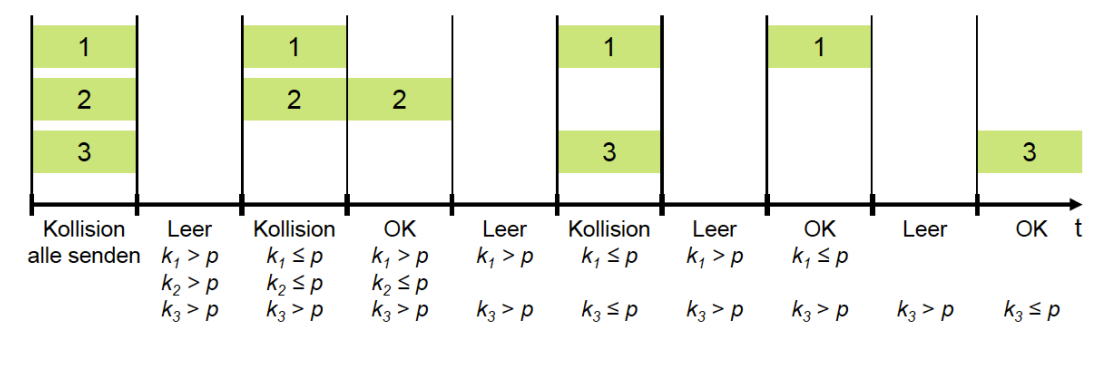
\includegraphics[width=14cm]{img/slotted1.png}
\end{figure}

\subsubsection{Erste Bewertung}
Es ist notwendig den Ablauf zu synchronisieren. Durch Synchronisation wird jedoch ein besserer Nutzungsgrad gegenüber Pure Aloha erreicht.

\subsubsection{Auslastung}
Angenommen wird eine hohe Anzahl Stationen N. Jede Station sendet Frames unabhängig von den vorangegangenen Frames. Alle Stationen senden Frames unabhängig voneinander.\\
Ein Frames wird genau dann erfolgreich übertragen, wenn: Eine Station sendet (Wahrscheinlichkeit hierfür beträgt p) und Gleichzeitig N–1 Stationen nicht senden (Wahrscheinlichkeit hierfür beträgt $(1–p)^{N–1}$) .\\
Daraus folgt Wahrscheinlichkeit für erfolgreiche Übertragung eines Frames 
	\begin{itemize}
	\item einer ausgewählten Station: $p*(1–p)^{N–1}$
	\item einer beliebigen aus N Stationen: $N*p*(1–p)^{N–1}$
	\end{itemize}
Optimalen Kanalsauslastung: 0,368

\subsection{Auswertung}
Wenn viele Stationen ein gemeinsames Medium nutzen, gilt: 
	\begin{itemize}
	\item Pure Aloha kann einen Kanal nur zu ca. 18$\%$ auslasten. 
	\item Slotted Aloha kann einen Kanal zu ca. 37$\%$ auslasten. 	
	\end{itemize}
Beide Raten sind nicht befriedigend. Suche nach Verbesserungen: Viele Kollisionen (aber nicht alle) ließen sich verhindern, wenn vor dem Beginn einer Aussendung überprüft würde, ob der Kanal frei ist. 

\subsection{CSMA}
Der \textbf{Ablauf} von Carrier Sense Multiple Access (CSMA):
	\begin{itemize}
	\item Sendewillige Station prüft, ob Kanal frei ist. 
	\item Wenn Kanal frei ist, wird Paket gesendet, aber nicht notwendigerweise sofort (Erklärung folgt). 
	\item Wenn Kanal belegt ist, kommen verschiedene Methoden zur Anwendung (Erklärung folgt). 
	\item Es kann zur Kollision kommen, wenn:
		\begin{itemize}
		\item Zwei Stationen gleichzeitig beginnen, zu senden (weil sie z.B. gewartet haben, bis Kanal frei ist). 
		\item Zwei Stationen kurz hintereinander mit dem Senden beginnen, aber durch die Signallaufzeit (Ausbreitungsgeschwindigkeit ist endlich) die andere Aussendung noch nicht "`angekommen"' ist (bisher bei Beschreibung von Aloha nicht berücksichtigt). 
		\end{itemize}
	\end{itemize}
Die Ausbreitung von Frames im Netzwerk kann so dargestellt werden:
	\begin{figure}[ht]
	\centering
	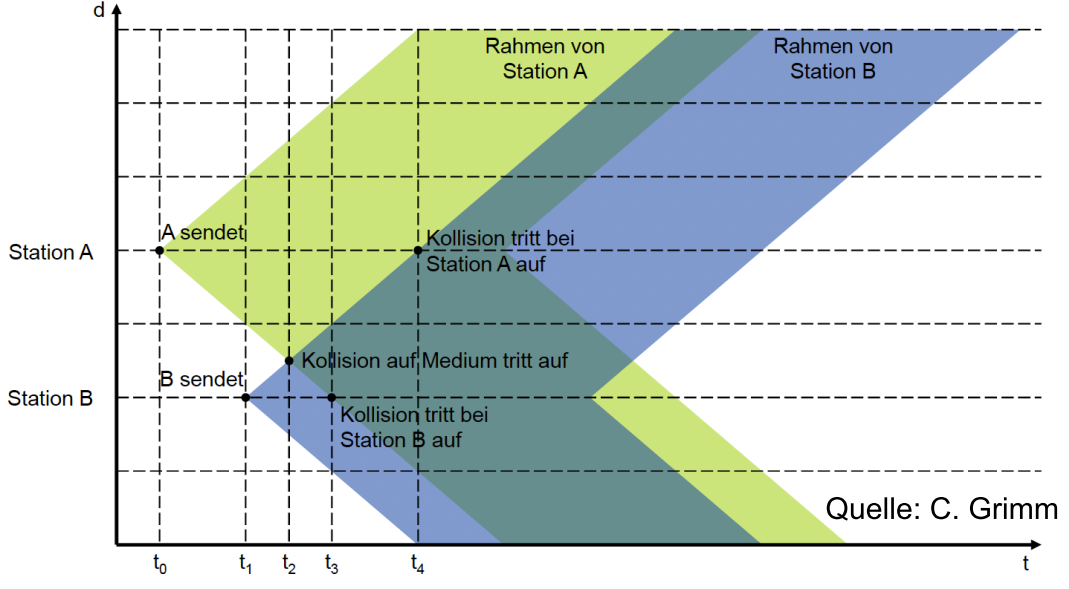
\includegraphics[width=10cm]{img/csma.png}
	\end{figure}
	
	
\noindent Grundsätzlich gibt es drei verschiedene \textbf{Methoden} für den Ablauf:
\subsubsection{1-persistent CSMA}	
	\begin{itemize}
	\item \textbf{Verhalten, wenn Kanal frei ist}: Sofortiges Aussenden
	\item \textbf{Verhalten, wenn Kanal belegt ist}: Warten, bis Kanal frei ist, dann sofortiges Aussenden,da es auf jeden Fall zur Kollision kommt, wenn mindestens zwei Stationen warten (beide senden wieder zum gleichen Zeitpunkt).
	\item \textbf{Verhalten bei Kollision}: Grundsätzlich wie bei Aloha, aber mit sich ändernder Wahrscheinlichkeit – siehe Backoff-Verfahren. 
	\end{itemize}
\subsubsection{Nonpersistent CSMA}	
	\begin{itemize}		
	\item \textbf{Verhalten, wenn Kanal frei ist}: Sofortiges Aussenden	
	\item \textbf{Verhalten, wenn Kanal belegt ist}: Zufällige Zeitspanne warten, dann Prüfung, ob Kanal frei ist. Bestimmung der zufälligen Zeit, wie bei Aloha. 	
	\item \textbf{Verhalten bei Kollision}: Grundsätzlich wie bei Aloha, aber mit sich ändernder Wahrscheinlichkeit – siehe Backoff-Verfahren. 	
	\end{itemize}	
\subsubsection{p-persistent CSMA}		
	\begin{itemize}	
	\item \textbf{Verhalten, wenn Kanal frei ist}:
		\begin{itemize}
		\item Senden mit Wahrscheinlichkeit p. 
		\item Mit Wahrscheinlichkeit (1-p) wird nicht gesendet, sondern gewartet. Wartezeit entspricht Übertragungsdauer zwischen den beiden entferntesten Stationen im Netz. 
		\item Bei nächster Überprüfung kann daher sicher die Aussendung einer anderen Station erkannt werden. 
		\end{itemize}	
	\item \textbf{Verhalten, wenn Kanal belegt ist}: Auf freien Kanal warten.  	
	\item \textbf{Verhalten bei Kollision}: Grundsätzlich wie bei Aloha, aber mit sich ändernder Wahrscheinlichkeit – siehe Backoff-Verfahren. 	
	\end{itemize}
	
\subsection{Ethernet - Verhalten bei Kollision}	
Die Kollisionserkennung erfolgt mit \textit{Carrier Sense Multiple Access / Collision detection}(CSMA/CD) und kann anhand des erhöhten Signalpegels erkannt werden. Bei einer Kollision wird Aussendung sofort abgebrochen und ein 48bit langes Jam-Signal (10101010 10101010 10101010) ausgesendet. Anschließend wird eine zufällige Zeit gewartet.\\
Durch das Abbrechen bei der Detektion einer Kollision kann Zeit gewonnen werden (Vergleich CSMA vs CSMA/CD).\\
Ist ein Frame zu kurz, kann auf Grund der Signallaufzeiten nicht immer zuverlässig eine Kollision erkannt werden. Jedoch ist eine Kollisionserkennung  notwendig, damit Aussendung wiederholt werden kann. Dabei ist die minimale Framelänge ist so zu dimensionieren, dass die maximale Round Trip Time (RTT) nicht unterschritten wird. Die maximale RTT hängt von der maximalen Ausbreitung des Mediums ab. \\
\textit{Eventuell Auffüllen von Frames – Erinnerung: Padding bei IEEE 802.3 Ethernet Frames, minimale Framelänge 64bit. Achtung, Hubs / Repeater gehen in die Zeit mit ein.}\\
\textbf{Erinnerung RoundTripTime:} Die minimale Übertragungsdauer eines Frames muss das doppelte der maximalen Laufzeit eines Signal zwischen den beiden entferntesten Stationen im Netz betragen – daher RTT. 
	
	\begin{figure}[ht]
	\centering
	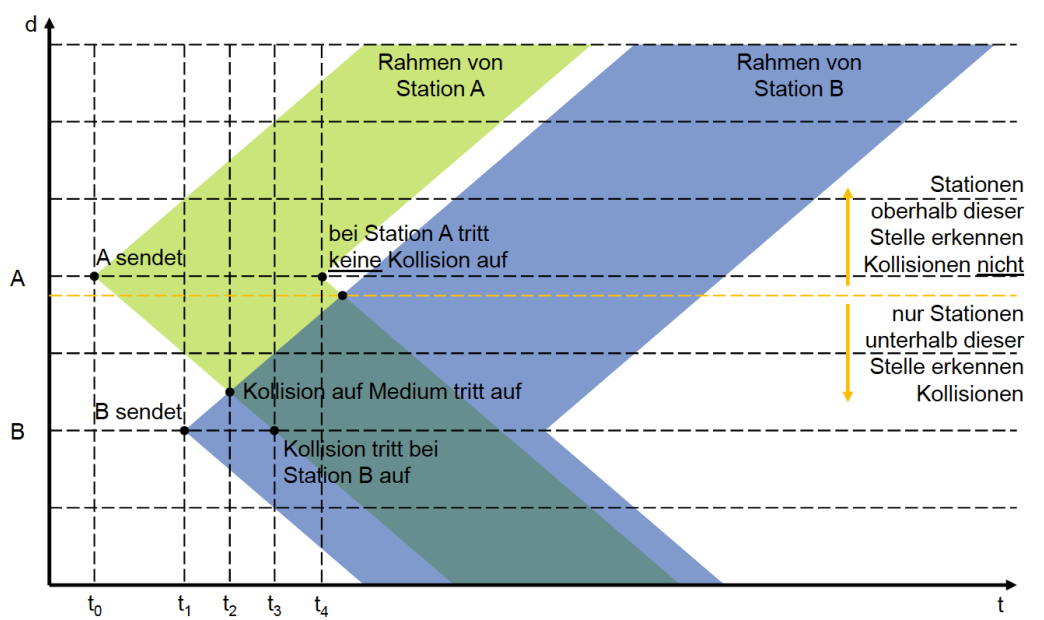
\includegraphics[width=11cm]{img/ethernetKollision.png}
	\end{figure}	
	
\subsection{Backoff-Verfahren}	
Nach Abbruch der Übertragung wegen einer erkannten Kollision würde es zu einer neuen Kollision kommen, wenn die beteiligten Stationen unmittelbar wieder mit dem Senden beginnen würden. Deshalb müssen die Stationen eine unterschiedliche lange Pause einlegen (so geschieht es auch bei Aloha über Wahrscheinlichkeit). 	\\

\noindent Das \textbf{Binary Exponential Backoff}: \\
Die Konfliktparteien wählen eine zufällige ganze Zahl \textbf{z}
 aus dem Intervall 0,$2^i$-1 (das sog. Contention Window), 
wobei i die Anzahl der bereits aufgetretenen Kollisionen dieser Station für das aktuelle Frame ist. Die Aussendung erfolgt nach z Slot Times. 

Bei Ethernet ist das Binary Exponential Backoff auf $2^{10}$  Möglichkeiten und 
maximal 16 Versuche begrenzt.  	

\subsection{CSMA/CA}
Bei der Carrier Sense Multiple Access / Collision Avoidance (CSMA/CA) soll eine Vermeidung von Kollisionen durch p-persistent Verfahren erreicht werden. (Es wird bei Vorhandensein von Daten mit Wahrscheinlichkeit p gesendet). Kollisionen können nicht völlig ausgeschlossen werden, jedoch muss der korrekter Empfang immer bestätigt werden, da Kollision vom Sender eventuell nicht bemerkt wird. \\

\noindent Häufig mit \textbf{RTS / CTS} (Ready-to-send / clear-to-send) kombiniert, wenn Hidden-Station-Problem zunimmt. Nicht immer lässt sich sicherstellen, dass alle Stationen die Aussendungen aller anderen Stationen empfangen können. Bei Funknetzen kann es daher zum Hidden-Station-Problem kommen. 

\noindent Ablauf bei RTS / CTS
	\begin{itemize}
	\item Sendewillige Station sendet RTS Frame aus. 
	\item Adressierte Station sendet beim Empfang des RTS Frames ein CTS Frame. 
	\item Alle Stationen in der Nähe, die RTS oder CTS empfangen sollen anschließend für die Dauer eines Datenframes nicht senden. \\
	\textit{RTS und CTS Frames enthalten eine Größenangabe für die Menge an Daten, die gesendet werden sollen. }
	
	\end{itemize}


% 365

\section{Mobile Netzwerke}

% 370, 380, 390, 400
%TODO Mobile Netzwerke


\section{Thomas Fragestunde}
\subsection{08.04}
	\begin{itemize}
		\item Merkmale von Verbindungen
		\begin{enumerate}
			\item Latenz
			\item Datenrate
			\item Jitter\\
			(Änderung der Latenz über die Zeit)
			\item Verfügbarkeit
			\item Fehlerrate
		\end{enumerate}
		\item Bandbreite wird in Hz und nicht in Mbit/s angegeben (Wlan bspw.)
		\item Ursachen für Jitter
			\begin{itemize}
				\item Es ist notwendig zu warten, bis gesendet werden kann
				\item Sich ändernde Routen, durch bspw. Wegänderungen, Datenaufteilung durch den Router
				\item Zeit, Route, Warteschlangenproblematik, gemeinsam genutzte Medien, CSMA
			\end{itemize}
		\item Warum Begrenzung der Übertragungsraten?
			\begin{itemize}
				\item Physikalisch - Frequenzen
			\end{itemize}
		\item Was begrenzt den max. Durchsatz eines Glasfaseranschlusses
			\begin{itemize}
				\item unterschiedlich lange Wege
				\item Kapazität (Zeit bis Ladung angekommen ist)
				\item Transistoren schalten nicht so schnell
				\item Signal-Rausch-Verhältnis
			\end{itemize}
	\end{itemize}
\subsection{09.04}
	\begin{itemize}
		\item Was begrenzt die Bandbreite?
			\begin{itemize}
				\item Kapazität $\rightarrow$ Grenzfrequenz
			\end{itemize}			
		\item CSACD
			\begin{itemize}
				\item Warten auf freies Medium
				\item Es gibt jedoch keine Garantien
				\item Verursacht Jitter
			\end{itemize}
		\item Jitter Gegenmaßnahmen
			\begin{itemize}
				\item Puffer (Warteschlange, FiFo)
				\item Pakete werden in gleichmäßiger Reihenfolge erhalten
			\end{itemize}
		\item Leitungs- vs. Paketorientiert
			\begin{itemize}
				\item ?
			\end{itemize}
		\item Möglichkeiten zur Beschreibung eines Standards
			\begin{itemize}
				\item textuell (schwer)
				\item Referenzimplementation (bspw. Bittorrent - aber berücksichtigt ggf. nicht alle Fälle)
				\item Automaten (5-Tupel, Mealy/Moore)
			\end{itemize}
		\item Zustandsbehaftete und zustandslose Protokolle
			\begin{itemize}
				\item Beispiel TCP (closed, SYN, etc.) besitzt einen Zustand
				\item Ein Zustand merkt sich die \glqq Vorgeschichte \grqq und damit was passiert ist. Somit ist ein Login immer zustandsbehaftet.
				\item Werden die Zwischenschritte nicht gespeichert, ist es zustandslos.
				\item Cookies bieten die Möglichkeit einen Zustand nachzurüsten.
			\end{itemize}
		\item Autonome Systeme sind \glqq Provider \grqq, die miteinander über \textit{Peering Points} verbunden sind
		\item Minimierung der Aufreihungslatenz
			\begin{itemize}
				\item Entsteht dadurch, dass das Paket erst versendet wird, wenn es vollständig da ist
				\item Lösung, Weiterleiten, sobald die ersten 6 Byte (Adresse) bekannt sind
			\end{itemize}
		\item Problem von CRC (cyclic redundancy check)?
			\begin{itemize}
				\item Es entsteht eine unnötige Belastung, wenn fehlerhafte Pakete weitergeleitet werden
			\end{itemize}
		\item Wann sollte umgeschaltet werden zwischen den verschiedenen Switch-Modi?
	\end{itemize}
\subsection{22.04}
	\begin{itemize}
		\item Implemenationen von Switches
			\begin{itemize}
				\item Shared Memorie
				\item Schaltmatrix (crossPoint $\rightarrow$ komplexe Schaltungen)
				\item Gemeinsamer Bus
			\end{itemize}
		\item Welche Geräte arbeiten auf welchen Layern?
			\begin{itemize}
				\item Layer 3: Router
				\item Layer 2: Switches
			\end{itemize}		
		\item Welche Dienste werden von welchen Layern erbracht?
			\begin{itemize}
				\item Layer 3: Routing, logische Adressierung
				\item Layer 2: Media Access
			\end{itemize}
		\item 
			\begin{itemize}
				\item 
			\end{itemize}
	\end{itemize}
\subsection{04.05}
	\begin{itemize}
		\item Routing?
		\begin{itemize}
			\item Erfolgt auf dem Network-Layer
			\item Dient der Kommunikation zwischen Geräten (IP kann als Protokoll genutzt werden)
			\item Ziele sind das Verbinden von Netzen miteinander und das Finden des richtigen Weges.
			\item IP bietet die Möglichkeit Netze logisch einzuteilen.
		\end{itemize}
		\item DNS (Domain Name System)
		\begin{itemize}
			\item Zum Auflösen einer Domain zu einer IP-Adresse
			\item Es gibt verschiedene Ebenen ...
			\item Beschreibung der Struktur: hierarchisch, mit Root, etc.
			\item Anfragen werden mitunter gecached
		\end{itemize}
		\item Migrationsstrategien von IPv4 nach IPv6\\
		(Tunneling, Dual Stack, Header Translation)
		\item Nachteile von Tunneling?
			\begin{itemize}
				\item mehr Header-Daten
				\item äußeres Protokoll bspw. nicht von Admins kontrolliert werden
			\end{itemize}
		\item Funktionsweise eines Routers
		\begin{itemize}
			\item Statisch (fest eingegebene Liste)
			\item Dynamisch (Routingprotkolle, Topologieermittlung, Pfaderkennung)
		\end{itemize}
		\item Möglichkeit zur Topologiebestimmung
		\begin{itemize}
			\item Es werden Testnachrichten (TTL=1) im Netzwerk versendet
			\item Auf diese Weise werden die Nachbarn bestimmt
			\item Anschließend erfolgt die Weitergabe dieser Informationen: n-Hob-Nachbarn
			\item Eine wichtige Bedingung hierbei ist, dass kein häufiger Wechsel erfolgt
		\end{itemize}
	\end{itemize}
	\subsection{13.05}
	\begin{itemize}
		\item Wie lange Routingverfahren brauchen um zu konvergieren hängt von der Größe der Netzwerke ab. Mögliche Lösungen sind
		\begin{itemize}
			\item Näherungsverfahren (Es muss nicht alles bekannt sein)
			\item pro- bzw. reaktives Routing: Abhängig davon, ob Kenntnisse über das Netz vorhanden sind, oder nicht
			\item Reduzierung der Graphenkomplexität - Einführen eines Backbones als \glqq minimal dominating set\grqq. Eine Menge, aus der alle Knoten erreichbar sind
		\end{itemize}
		\item Das Count-to-infinity-Problem kann durch einen Distanzvektor behoben werden
		\item Netzwerkparameter, die die Güte beschreiben: Datenrate, Datensatz, Fehlerrate
		\item Was ist zu tun, wenn mehr Bedarf als Ressourcen bestehen
		\begin{itemize}
			\item Flusskontrolle
			\item Prioritäten festlegen \\
			(Ein Gespräch sollte eine Latenz von unter 1/45 Sekunden haben, 64 kbit/s + Header)
		\end{itemize}
	\end{itemize}	
	\subsection{18.05}
	\begin{itemize}
		\item Gegen was wirkt die FiFo-Queue?\\
		$\rightarrow$ Zur Jitter-Bekämpfung, bewirkt dafür aber Latenz
		\item Ursachen für Verzögerungen auf Layer 2 (Ethernet)
		\begin{itemize}
			\item Shared Medium
			\item Alle Teilnehmer senden, dadurch kommt es Kollisionen, die Teilnehmer müssen warten/lauschen/nach einer zufälligen Zeit erneut senden
		\end{itemize}
		\item Beispielhafte Übertragungsraten
		\begin{itemize}
			\item Audio CD
				\begin{itemize}
					\item 44,1 kHz Abtastfrequenz, 16 Bit Abtastung (geringer Quantisierungsfehler), *2 (Stereo)
					\item 1,5 Mbit/s ohne Fehlerkorrektur
				\end{itemize}
			\item Video 10-100 Mbit/s
			\item Tippgeschwindigkeit: 200-300 Anschläge die Minute
		\end{itemize}
		\item Ursachen für Latenz
		\begin{itemize}
			\item Entfernung, Router/Switches, Aufreihung, Pakete erst abgesendet, wenn voll
		\end{itemize}
	\end{itemize}
	\subsection{25.05?}
	\begin{itemize}
		\item RTP (Real-Time Transport Protocol)?
		\begin{itemize}
			\item zur kontinuierlichen Übertragung von audiovisuellen Daten
			\item Normalerweise über UDP
			\item ? Kommt es zu einem zu hohen Verlust, erfolgt ein Kodecwechsel
		\end{itemize}
	\end{itemize}
	\subsection{03.06}
	\begin{itemize}
		\item SMTP/POP3
		\begin{itemize}
			\item Via TCP (Layer 4)
			\item Port 25,584
			\item Thomas erwartete detailiertes Wissen (bspw. befindet sich am Ende ein Punkt, etc.)
			\item Sicherheit, Authentizität,... gibt es nicht
		\end{itemize}
		\item Zustandsbehaftete Protokolle sind: POP3, IMAP, TCP, FTP
		\item IMAP4
		\begin{itemize}
			\item Port 143
			\item neuer und bietet Verwaltung, Ordner, etc.
			\item \glqq Besser\grqq als POP3 und arbeitet auf dem Server (suchen, kopieren, etc.)
		\end{itemize}
		\item Sinn von Subnetzmasken?
		\begin{itemize}
			\item Anhand der Ziel-, der eigenen Adresse und der Netzmaske kann entschieden werden, ob sich der Empfänger im eigenen Netzwerk oder außerhalb befindet
		\end{itemize}
		\item Nutzung von UPnP: Fernseher, Smartphones, Playstation, DSL-Router, Drucker, etc.
		\item ICMP?
		\begin{itemize}
			\item Steuerungsnachrichten für Geräte im Internet
			\item Meldungen, wenn Nachricht nicht zugestellt wurde (Host, Port, etc. unreachable)
			\item TTL abgelaufen (bei IP-Paketen)
			\item EchoRequest \& EchoReply
			\item \glqq Mach-mal-langsam\grqq Nachrichten			
		\end{itemize}
		\item Routingprotokolle
		\begin{itemize}
			\item Topologieerkennung
			\item Topologieverbreitung
			\item günstigste Wege finden (Kostenfunktion)
			\item Distanzvektorproblem
			\item CountToInfinity $\rightarrow \infty = 16$
		\end{itemize}
		\item typische Protokollfragen
		\begin{itemize}
			\item VLAN
			\item HTTP
			\item FTP
			\item Die zwei Modi von Switches
			\item Routing Protokoll
		\end{itemize}		
	\end{itemize}
	\subsection{15.06}
	\begin{itemize}
		\item Wie groß sollten LAN-Segmente gewählt werden?
		\begin{itemize}
			\item Nachteile von groß: Broadcast Domain
			\item Nachteile von klein: Mehr Routing, mehr verpacken, Aufreihungslatenz, Prüfsummen, mehr Overhead
		\end{itemize}
		\item Anforderungen an das Networkfilesystem (NFS): sicher, transparent, Mehrbenutzerbetrieb, schnell, Latenz
		\item RFC Lebenszyklus: ?
		%TODO Hier gibt es auch noch was zu tun (was, das weiß nur Christian)
		\item XMPP
		\begin{itemize}
			\item basiert auf XML zum Nachrichtenaustausch
			\item Ende-zu-Ende chatten
			\item Geringe Datenübertragungsrate (Chat, ohne Bilder)
			\item Character-Encoding
			\item Anwesenheitserkennung (on, off, tipping)
		\end{itemize}
	\end{itemize}
	\subsection{17.06}
	\begin{itemize}
		\item Was ist P2P?
		\begin{itemize}
			\item direkte Kommunikation via Vermittlungsstellen
			\item Verfügbarkeit: auf einem PC (Lösung: Replikation)
			\item dezentral: keine legislativen/judikativen Entscheidungen
			\item Lastverteilung
		\end{itemize}
		\item WebDav
		\begin{itemize}
			\item Web-based Distributed Authoring and Versioning
			\item Standard zur Bereitstellung von Dateien im Internet
			\item setzt auf HTTP auf - und fügt hinzu
			\item Mit WebDAV können ganze Verzeichnisse übertragen werden.
			\item Einsatz für CMS
		\end{itemize}
		\item Angaben von RoutNameServern für Topleveldomains
		\begin{itemize}
			\item Country: de,...
			\item General: edu, org,...
		\end{itemize}
		\item LDAP?
		\begin{itemize}
			\item hierarchische Datenbank
			\item Aktives Verzeichnis: Nutzergruppenverwaltung
		\end{itemize}
		\item Aufgabe des Sessionlayers
		\begin{itemize}
			\item Zusammenfassung der verschiedenen Kommunikationspfade
			\item Nutzung der Zustände (-behaftete: SSH,FTP,TCP,IMAP4,POP3)
		\end{itemize}
		\item Begriff Authentisierung
		\begin{itemize}
			\item "Dem System klar machen wer man ist"
			\item Biometrisch, Token, Schlüssel, wissensbasiert
		\end{itemize}		
	\end{itemize}
	\subsection{24.06}
	\begin{itemize}
		\item Kerberos 
		\begin{itemize}
			\item Kerberos ist ein verteilter Authentifizierungsdienst
			\item Kerberos soll eine sichere und einheitliche Authentifizierung in einem ungesicherten TCP/IP-Netzwerk auf sicheren Hostrechnern bieten.
		\end{itemize}
		\item Medienzugriff auf Layer 2
		\begin{itemize}
			\item Aloa (Bei Zugriff wird einfach zugerufen)
			\item Slotted Aloa (Zugriff nur zu bestimmten Zeiten, dadurch geringere Kollisionen)
			\item Bei Ethernet: CSMACD
			\begin{itemize}
				\item Carrier Sense (Lauschen auf dem Medium)
				\item Multiple Access
				\item Collision Detection 
			\end{itemize}
			\item Pure Aloa
			\item GSM als kollisionsfreies Zugriffsverfahren (sobald die Verbindung besteht - auf Grund des exklusiven Medienzugriffs??)
		\end{itemize}
		\item Multiplexverfahren
		\begin{itemize}
			\item Methoden zur Signal- und Nachrichtenübertragung, bei denen mehrere Signale zusammengefasst und simultan über ein Medium übertragen werden.\\
			(Raum, Frequenz, Zeit, Code)
		\end{itemize}
	\end{itemize}
	\subsection{29.06}
	\begin{itemize}
		\item Faktoren die in eine Kostenfunktion beim Routing miteinbezogen werden können
		\begin{itemize}
			\item Topologiekenntnisse
			\item Durchsatz/Datenrate
			\item Latenz
			\item Reale Kosten
		\end{itemize}
		\item Dijkstra Algorithmus
		\item Hidden Station Problem
		\begin{itemize}
			\item RTC/CTS lohnt sich, wenn die Pakete klein genug sind - verglichen zu den Nutzerdaten
			\item OLSR (Optimized Link State Routing)\\
			(Reduzierung der Graphenkomplexität - Backbone Bildung)
		\end{itemize}
	\end{itemize}
	\subsection{08.07}
	\begin{itemize}
		\item MIB (bei SNMP)
		\begin{itemize}
			\item Management Information Base (deutsch: Verwaltungsinformationsbasis) beschreibt die Informationen, die über ein Netzwerk-Management-Protokoll abgefragt oder modifiziert werden können.
			\item Das Simple Network Management Protocol ist ein Netzwerkprotokoll, um Netzwerkelemente von einer zentralen Station aus überwachen und steuern zu können. 
			\item Es werden Schlüssel beschrieben, die zur Speicherung des \glqq Gesundheitszustandes\grqq von Geräten dienen.
			\item Eine MIB-Datenbank erklärt, für welche Information ein Schlüssel steht.
		\end{itemize}
		\item Hemming-Distanz
		\begin{itemize}
			\item Der Hamming-Abstand ist ein Maße für die Unterschiedlichkeit von Zeichenketten. 
			\item Die Distanz zweier Blöcke mit fester Länge ist dabei die Anzahl der unterschiedlichen Stellen.
			\item HD wird zur Fehlererkennung und zur Fehlerkorrektur benutzt.
			\item Ob eine Fehlererkennung oder -korrektur stattfinden kann, hängt von der Hamming-Distanz ab.
			\item FEC - forward error correction
			\begin{itemize}
				\item Am einfachsten: 2-3 mal senden
				\item Fehler erkennen: Distanz von 2
				\item Fehler korrigieren: Distanz von 3
			\end{itemize}
		\end{itemize}
		\item Aktives vs. passives Scanning
		\begin{itemize}
			\item Passiv: Der AP sendet Beacons mit Daten aus
			\item Aktiv: Der Client fragt beim AP nach
			\item Wenn ein Client wechseln möchte, wäre er solange offline bis er ein Beacon erhalten würde. Durch aktives nachfragen kann die \glqq Hand off\grqq Zeit reduziert werden.
		\end{itemize}
		\item RTS/CTS (Ready to send / clear to send)
		\item Bluetooth
		\begin{itemize}
			\item Musik, Staubsauger, Eingaben, Smartwatches, Datenübertragung,...
			\item Kopfhörer Datenübertragung
			\begin{itemize}
				\item Bits pro Sekunde = Samplerate * Samplebreite * Kanäle
				\item 2*48 kHz (Nyquist) - Audio-CD: 44,1 kHz
				\item 16 Bit
				\item 2 Kanäle
				\item $\approx$ 140/150 kBit/s
			\end{itemize}
		\end{itemize}
	\end{itemize}
	
	

\newpage
\begin{multicols}{2}
	\addcontentsline{toc}{section}{Literatur}
	\nocite{*}
	\bibliographystyle{plain}
	\bibliography{literatur}
\end{multicols}

\newglossaryentry{arpa}{name=ARPA,description={Advanced Research Projects Agency}}
\newglossaryentry{icann}{name=ICANN,description={Internet Corporation for Assigned Names and Numbers}}
\newglossaryentry{ietf}{name=IETF,description={Internet Engineering Task Force}}
\newglossaryentry{ripe}{name=RIPE,description={Réseaux IP Européens}}
\newglossaryentry{ripencc}{name=RIPE NCC,description={RIPE Coordination Centre}}
\newglossaryentry{denic}{name=DENIC,description={Deutsches Network Information Center}}
\newglossaryentry{dns}{name=DNS,description={Domain Name System}}
\newglossaryentry{udp}{name=UDP,description={User Datagram Protocol}}
\newglossaryentry{tcp}{name=TCP,description={Transmission Control Protocol}}
\newglossaryentry{atdn}{name=ATDN,description={AOL Transit Data Network}}
\newglossaryentry{gx}{name=GX,description={Global Crossing}}
\newglossaryentry{decix}{name=DE-CIX,description={German Commercial Internet Exchange}}
\newglossaryentry{http}{name=HTTP,description={Hypertext Transfer Protocol}}
\newglossaryentry{tftp}{name=TFTP,description={Trivial File Transfer Protocol}}
\newglossaryentry{ftp}{name=FTP,description={File Transfer Protocol}}
\newglossaryentry{smtp}{name=SMTP,description={Simple Mail Transfer Protocol}}
\newglossaryentry{mac}{name=MAC,description={Medium Access Control}}
\newglossaryentry{crc}{name=CRC,description={Cyclic Redundancy Check}}
\newglossaryentry{csmacd}{name=CSMA/CD,description={Carrier Sense Multiple Acces / Collision Detection}}
\newglossaryentry{fdd}{name=FDD,description={Frequency Divsion Duplex}}
\newglossaryentry{tdd}{name=TDD,description={Time Division Duplex}}
\newglossaryentry{sfd}{name=SFD,description={Start Frame Delimiter}}
\newglossaryentry{atm}{name=ATM,description={Asynchronous Transfer Mode}}
\newglossaryentry{tpid}{name=TPID,description={Tag Protocol Identifier}}
\newglossaryentry{cfi}{name=CFI,description={Canonical Formati Indicator}}
\newglossaryentry{vid}{name=VID,description={VLAN Identifier}}
\newglossaryentry{nat}{name=NAT,description={Network Address Translation}}
\newglossaryentry{cidr}{name=CIDR,description={Classless Inter-Domain Routing}}
\newglossaryentry{dhcp}{name=DHCP,description={Dynamic Host Configuration Protocol}}
\newglossaryentry{tos}{name=ToS,description={Type of Service}}
\newglossaryentry{ttl}{name=TTL,description={Time to Live}}
\newglossaryentry{snmp}{name=SNMP,description={Simple Network Management Protocol}}
\newglossaryentry{vpi}{name=VPI,description={Virtual Path Identifier}}
\newglossaryentry{vci}{name=VCI,description={Virtual Channel Identifer}}
\newglossaryentry{uri}{name=URI,description={Uniform Resource Identifier}}
\newglossaryentry{urn}{name=URN,description={Uniform Resource Name}}
\newglossaryentry{url}{name=URL,description={Uniform Resource Locator}}
\newglossaryentry{tld}{name=TLD,description={Top Level Domain}}
\newglossaryentry{cctld}{name=ccTLD,description={Country Code Top Level Domain}}
\newglossaryentry{gtld}{name=gTLD,description={Generic Top Level Domain}}
\newglossaryentry{nicdns}{name=NIC,description={Name Information Center}}
\newglossaryentry{nic}{name=NIC,description={Network Interface Controller}}
\newglossaryentry{ace}{name=ACE,description={ASCII Compatible Encoding}}
\newglossaryentry{ntp}{name=NTP,description={Network Time Protocol}}
\newglossaryentry{sntp}{name=SNTP,description={Simple Network Time Protocol}}
\newglossaryentry{www}{name=WWW,description={World Wide Web}}
\newglossaryentry{tls}{name=TLS,description={Transport Layer Security}}
\newglossaryentry{sctp}{name=SCTP,description={Stream Control Transmission Protocol}}
\newglossaryentry{ssh}{name=SSH,description={Secure Shell}}
\newglossaryentry{nvt}{name=NVT,description={Network Virtual Terminal}}
\newglossaryentry{rsa}{name=RSA,description={Rivest, Shamir und Adleman}}
\newglossaryentry{pdu}{name=PDU,description={Packet Data Unit}}

\newpage
\addcontentsline{toc}{section}{Glossar}
\begin{multicols}{2}
	\glsaddall
	\printglossary[title=Glossar,toctitle=Glossar]
\end{multicols}

\end{document}